\documentclass[12pt,a4paper,oneside]{report}
\usepackage[a4paper,margin=1in]{geometry}
\usepackage{graphicx}
\usepackage{hyperref}
\usepackage{fontspec}
\usepackage{fvextra}
\usepackage{tabularx}
\usepackage{array}
\usepackage{pdflscape}
\usepackage{microtype}
\usepackage{eso-pic}
\usepackage{tikz}
\usepackage{tocloft}
\newcolumntype{Y}{>{\raggedright\arraybackslash}X}
\setlength{\parindent}{0pt}
\setlength{\parskip}{0.55em}
\setlength{\emergencystretch}{3em}
\setlength{\cftparskip}{0pt}
\setlength{\cftbeforefigskip}{0.65em}
\setlength{\cftbeforetabskip}{0.65em}
\setcounter{secnumdepth}{3}
\setcounter{tocdepth}{2}
\hypersetup{hidelinks,pdftitle={Investigating Coordination Signals in Multi-Agent Tool-Using Language Models},pdfauthor={Dhruva N}}
\renewcommand{\bibname}{References}
\newcommand{\addreportpageborder}{%
  \AddToShipoutPictureBG*{%
    \begin{tikzpicture}[remember picture,overlay]
      \draw[line width=4pt]
        ([xshift=0.82in,yshift=-0.82in]current page.north west)
        rectangle
        ([xshift=-0.82in,yshift=0.82in]current page.south east);
    \end{tikzpicture}%
  }%
}
\begin{document}
\begin{titlepage}
\addreportpageborder
\begin{center}

\includegraphics[height=2.1cm]{Images/pes_logo.png}\\[0.45cm]
\textbf{\Large Dissertation on}\\[0.65cm]
\textbf{\Huge Investigating Coordination Signals in Multi-Agent Tool-Using Language Models}\\[0.55cm]
Submitted in partial fulfilment of the requirements for the award of the degree of\\[0.65cm]
\textbf{\Large Master of Technology in}\\[0.35cm]
\textbf{\Large Data Science \& Artificial Intelligence}\\[0.65cm]
\textbf{Course -- UE19CS651}\\[0.15cm]
\textbf{Semester -- Fourth Semester; Project Phase - 2}\\[0.65cm]
\textbf{Submitted by:}\\[0.2cm]
\textbf{Dhruva N}\\[0.15cm]
\textbf{PES2PGE23DS169}\\[0.65cm]
Under the guidance of\\[0.2cm]
\textbf{Dr. Milan Joshi}\\[0.15cm]
Faculty - Great Learning\\[0.65cm]
May 2026 -- October 2026\\[0.65cm]
\textbf{DEPARTMENT OF ARTIFICIAL INTELLIGENCE AND MACHINE LEARNING}\\[0.2cm]
FACULTY OF ENGINEERING\\[0.15cm]
PES UNIVERSITY
\vfill
{\footnotesize
(Established under Karnataka Act No. 16 of 2013)\\
Electronic City, Hosur Road, Bengaluru -- 560 100, Karnataka, India
}
\end{center}
\end{titlepage}
\clearpage
\addreportpageborder
\thispagestyle{empty}
\begin{center}

\includegraphics[height=1.3cm]{Images/pes_logo.png}\\[0.1cm]
\textbf{\Large PES UNIVERSITY}\\
(Established under Karnataka Act No. 16 of 2013)\\
Electronic City, Hosur Road, Bengaluru -- 560 100, Karnataka, India\\[0.4cm]
\textbf{FACULTY OF ENGINEERING}\\[0.5cm]
\textbf{\Large CERTIFICATE}\\[0.4cm]
\end{center}
This is to certify that the dissertation entitled \textbf{``Investigating Coordination Signals in Multi-Agent Tool-Using Language Models''} is a bonafide work carried out by \textbf{Dhruva N (PES2PGE23DS169)} in partial fulfilment for the completion of the Fourth Semester Project Phase - 2 (UE19CS651) in the Program of Study -- Master of Technology in Data Science \& Artificial Intelligence at PES University, Bengaluru, during May 2026 -- October 2026.
\vspace{1.2cm}
\begin{center}
\begin{minipage}[t]{0.30\textwidth}\centering\rule{0.9\linewidth}{0.4pt}\\Dr. Milan Joshi\\Faculty - Great Learning\end{minipage}\hfill
\begin{minipage}[t]{0.30\textwidth}\centering\rule{0.9\linewidth}{0.4pt}\\Dr. Sandesh B J\\Chairperson\end{minipage}\hfill
\begin{minipage}[t]{0.30\textwidth}\centering\rule{0.9\linewidth}{0.4pt}\\Dr. Keshavan B K\\Dean of Faculty\end{minipage}
\end{center}
\vspace{1.4cm}
\begin{center}
\begin{minipage}[t]{0.42\textwidth}\centering\rule{0.9\linewidth}{0.4pt}\\Prof. Jawahar Doreswamy\\Chancellor\end{minipage}\hfill
\begin{minipage}[t]{0.42\textwidth}\centering\rule{0.9\linewidth}{0.4pt}\\Dr. Suryaprasad J\\Vice Chancellor\end{minipage}
\end{center}
\vspace{5cm}
\textbf{External Viva}\\[0.3cm]
Name of the Examiners\hfill Signature with Date\\[0.7cm]
1.\rule{0.4\textwidth}{0.4pt}\hfill\rule{0.4\textwidth}{0.4pt}\\[0.5cm]
2.\rule{0.4\textwidth}{0.4pt}\hfill\rule{0.4\textwidth}{0.4pt}
\clearpage
\ClearShipoutPictureBG
\chapter*{Declaration}
\addcontentsline{toc}{chapter}{Declaration}
I hereby declare that the Project Phase - 2 entitled \textbf{``Investigating Coordination Signals in Multi-Agent Tool-Using Language Models''} has been carried out by me under the guidance of Dr. Milan Joshi, Faculty - Great Learning, and submitted in partial fulfilment of the course requirements for the award of the degree of Master of Technology in Data Science \& Artificial Intelligence of PES University, Bengaluru, during the academic semester May 2026 -- October 2026. The matter embodied in this report has not been submitted to any other university or institution for the award of any degree.
\vspace{2cm}
\begin{flushright}
PES2PGE23DS169\hspace{1.5cm}Dhruva N\\[1.2cm]
\rule{0.45\textwidth}{0.4pt}\\Signature
\end{flushright}
\clearpage
\chapter*{Acknowledgement}
\addcontentsline{toc}{chapter}{Acknowledgement}
I express my sincere gratitude to my mentor, Dr. Milan Joshi, Faculty - Great Learning, for guidance and mentorship throughout this project. I also thank Dr. Sandesh B J, Chairperson, and Dr. Keshavan B K, Dean of Faculty, for their support. I acknowledge the leadership of Prof. Jawahar Doreswamy, Chancellor, and Dr. Suryaprasad J, Vice Chancellor, and thank PES University for the academic setting in which this work was completed.
\clearpage
\chapter*{Abstract}
\addcontentsline{toc}{chapter}{Abstract}
\label{abstract}
Coordination in multi-agent language-model systems is difficult to assess: a successful group outcome does not show how agents’ actions relate, and shared feedback can conceal individual contributions. Tool-use studies can make actions and task-state changes visible, but explicit traces alone do not establish coordination. The study asked how single-agent, independent multi-agent, and coordination-oriented policies differed in completion, action use, and stopping behavior in a controlled tool-use task. An initial repeated guessing-game implementation was followed by a synthetic bug-fix experiment using three model-backed policies, 16 fixture variants, and four repetitions per policy-fixture combination. In total, 192 completed episodes were examined through tool-event logs, outcome summaries, and categorical action-profile analysis; a later replay check tested recorded guessing-game transitions. Full success was recorded in 187 episodes (97.4\%); five were partial, and none failed. Success rates were 100\% for the single-agent policy, 93.75\% for independent multi-agent, and 98.44\% for coordination-oriented policy, while all five partial episodes involved premature finalization on billing fixtures despite remaining call budget. The action-profile estimates showed small associations with outcomes but remained exploratory because they were based on sparse categories. The results show that explicit action traces support auditing and descriptive comparisons in this synthetic setting, but do not establish policy superiority or causal coordination. The study contributes an auditable tool-use framework and identifies participation and stopping behavior as candidates for future validation; it does not replicate information-theoretic findings about emergence.

\clearpage
\tableofcontents
\clearpage
\begingroup
\setlength{\parskip}{0pt}
\listoffigures
\endgroup
\clearpage
\begingroup
\setlength{\parskip}{0pt}
\listoftables
\endgroup
\clearpage\chapter{Paper Premise and Research Aims}
\label{chapter-01}
\thispagestyle{plain}
\section{From a collection to a collective}
The motivating question in Christoph Riedl’s paper, \emph{Emergent Coordination in Multi-Agent Language Models}, is when agents form an integrated collective rather than merely acting side by side. A group may produce an aggregate result while its members make interchangeable guesses or react independently to shared feedback. The paper instead looks for higher-order structure: relationships among evolving agent states that carry information about the group’s future and task-relevant behavior beyond what separate agents reveal (Riedl, 2026, pp. 1–2). This is an informational and behavioral criterion, not a claim of group minds or human-like understanding. Task success alone does not establish collective integration, and a coordination statistic alone does not establish improved performance. The framework draws on information-theoretic approaches to emergence and collective intelligence (Rosas et al., 2020; Riedl et al., 2021).

\section{The paper’s terms}
\textbf{Emergence} here means that a system-level or future-state property contains information not recoverable from the component agents considered independently. The paper studies dynamical emergence: whether current agent states jointly predict a future collective state beyond what separate components explain (Riedl, 2026, pp. 2, 4–5; Rosas et al., 2020).

\textbf{Synergy} is information about a target available only from joint sources, not from any one source alone. In partial information decomposition (PID), it is distinguished from information unique to a source and \textbf{redundancy}, the overlap in information across sources (Williams and Beer, 2010; Riedl, 2026, pp. 2, 4). PID is a family of decompositions rather than a single consensus estimator: formulations differ in how they operationalize redundant and synergistic information (Kolchinsky, 2022; Newman et al., 2022; Varley, 2024). Neither synergy nor redundancy is synonymous with team performance. Redundant information may reflect shared signal, but the paper asks whether it aligns agents with a task-relevant group state.

\textbf{Differentiation} means agents have distinct, relatively persistent contribution patterns or trajectories; the paper assesses it separately from PID with hierarchical models of equal-share deviations and their change over time (Riedl, 2026, pp. 5–6). \textbf{Alignment} is organization around a shared, task-relevant signal rather than coupling from common timing or feedback alone. \textbf{Complementarity} is differentiated contribution that is jointly useful for the common objective. The framework therefore separates information structure, agent-specific behavior, task linkage, and interpretation. The paper cautions that structural synergy does not imply sophisticated cognition (Riedl, 2026, pp. 3, 7–10).

\section{A minimal task that exposes coordination}
In the paper’s group binary-search task, agents privately propose integers; their guesses are summed and compared with a hidden target. They cannot see peers’ guesses or know group size. After each round, all receive only the shared “too high” or “too low” result; a correct sum ends the task (Riedl, 2026, p. 3; Goldstone et al., 2024).

This information restriction makes coordination measurable without direct messages. Shared feedback says something about the aggregate but does not identify any agent’s contribution. Identical independent adjustments can produce redundant guesses or overshooting, while differentiated guesses could compensate for one another. The repeated trajectory provides observations of individual behavior, group dynamics, and progress toward a clear numerical goal. Yet common feedback can synchronize agents without producing useful complementarity, so success alone is not the paper’s measure of coordination (Riedl, 2026, pp. 3–5).

\section{Interventions and research questions}
The paper compares three interventions: \textbf{Plain}, the task-only control; \textbf{Persona}, which assigns each agent a persona with background, skills, personality, and values; and \textbf{theory of mind (ToM)}, which adds an instruction to consider others’ likely actions and their effects on the group result (Riedl, 2026, pp. 2–3). The question is whether prompts shape coordination, not simply raise an aggregate score.

The paper organizes the study around three questions (Riedl, 2026, pp. 2–3):

\begin{enumerate}
\item \textbf{RQ1:} Do multi-agent LLM systems possess the capacity for emergence?
\item \textbf{RQ2:} What functional advantages, such as synergistic coordination and higher performance, arise when emergence occurs?
\item \textbf{RQ3:} Can prompts, roles, and reasoning structures steer coordination toward outcome-relevant, goal-directed synergy?
\end{enumerate}
Together, these are the \textbf{motivating paper’s questions}, not questions this project can answer with its Phase 2 experiment. The project’s synthetic task, policy conditions, and analyses differ from the paper’s. The following project questions were formulated retrospectively after examining the final-run results; they are descriptive questions, not a priori hypotheses:

\begin{enumerate}
\item \textbf{Project RQ1 --- Completion:} Within the synthetic bug-fix environment, how do the single-agent, independent multi-agent, and prompted-coordination policies differ in full completion, partial completion, and failure across the matched fixture assignments?
\item \textbf{Project RQ2 --- Action use:} How do these policies differ in tool-call volume, tool mix, and (for the two multi-agent conditions) distribution of actions between agents?
\item \textbf{Project RQ3 --- Stopping behavior:} How do these policies differ in tool calls through finalization and in premature finalization, defined as ending with a required fixture defect unresolved?
\end{enumerate}
The Phase 2 outcomes and traces directly describe these quantities. They support comparisons within this model, dataset, and environment, but do not identify causal effects or answer the paper’s questions about emergence, synergy, or general-purpose coordination. Section 10.7 returns to each project question explicitly.

\section{Analyses that inform this project}
The paper’s \textbf{time-delayed information} analyses ask how current agent states relate to future states, using principally a one-round lag to capture predictability and oscillation. In the pairwise emergence-capacity test, two agents’ current states predict their joint future state. PID separates unique, redundant, and synergistic predictive information; synergy is the part unavailable from either source alone (Riedl, 2026, pp. 4–5; Luppi et al., 2022; Williams and Beer, 2010). This is predictive structure, not causal evidence by itself. Other higher-order information measures, including dynamical O-information, address related but distinct questions and should not be treated as interchangeable with PID (Stramaglia et al., 2021; Varley, 2026).

A \textbf{practical criterion} tests whether agent states predict a task-relevant macro-signal: group error from the hidden target. The paper compares this with the macro-signal’s own predictability. Its coalition analysis asks whether a triplet predicts the future macro-signal beyond the best pair, denoted by \$I\allowbreak\_3\$ and \$G\allowbreak\_3\$ (Riedl, 2026, pp. 4–5). Guesses are transformed into deviations from an equal-share contribution, helping distinguish progress toward the goal from agents merely fluctuating together (Riedl, 2026, p. 5).

\textbf{Agent differentiation} is evaluated separately with hierarchical models of agent-specific contribution levels and time slopes, controlling for group-wide temporal changes. This distinguishes persistent identity-linked differences from shared feedback responses or different rates of change; difference alone does not establish synergy (Riedl, 2026, pp. 5–6).

The \textbf{falsification and null tests} probe alternative explanations. Row-wise shuffles disrupt agent identity-to-contribution pairings; time/column block shuffles preserve aspects of individual dynamics while breaking cross-agent temporal alignment. Detrending, functional baselines, and estimator sensitivity checks address shared trends, autocorrelation, and finite-sample bias (Riedl, 2026, pp. 5–6; Appendix A.4). These tests make the claims falsifiable; no single surrogate proves a mechanism.

\section{Conclusions, limits, and the project boundary}
In the paper’s main experiments, dynamical emergence appears across conditions, but the ToM condition shows stronger stable task alignment and identity-linked differentiation than Plain or Persona. The paper associates personas with differentiated behavior and the additional other-agent reasoning prompt with its strongest evidence of goal-directed complementarity. Neither synergy nor redundancy alone is reported as sufficient for performance; their interaction is associated with improved performance. The estimated indirect ToM effect through synergy is marginal in the main text, not definitive mediation evidence (Riedl, 2026, pp. 7–9).

Additional model experiments vary in results. Limitations remain: one deliberately minimal task; short, discrete trajectories that make information estimates sensitive to estimator and binning choices; some analyses restricted to pairwise, order-two synergy; and early stopping that entangles task success with time available for coordination. The authors also note that synergy and redundancy are co-dependent and difficult to link cleanly to performance, calling for research across more tasks and measures (Riedl, 2026, pp. 5, 9–10). These conclusions describe the paper’s experiments, not a general law.

The repository’s phases are distinct from these paper findings. Phase 1 adapts a guessing game, but evidence does not establish reproduction of the full intervention matrix or analytical framework. Phase 2 changes the task to synthetic bug fixing, with explicit tool actions and fixture outcomes. Its active analysis relates categorical action profiles to episode outcomes; it does not implement the paper’s time-delayed PID, macro-signal criteria, or differentiation models (coordination\allowbreak\_analysis.py; Riedl, 2026, pp. 4–6). Work examining synergistic representations inside a single LLM addresses within-model information organization, a different level of analysis from interactions among agents (Urbina-Rodriguez et al., 2026). The final Phase 2 run has 192 completed episodes: 187 successes and 5 partials. Retry records are not additional episodes (aggregate\allowbreak\_summary.json).

The tool-use extension was considered to make actions, state transitions, and outcomes more explicit and auditable. It improves control and observability in a changed task; it does not directly test whether the paper’s conclusions generalize or reproduce its emergence constructs.

\begin{figure}[htbp]
\centering
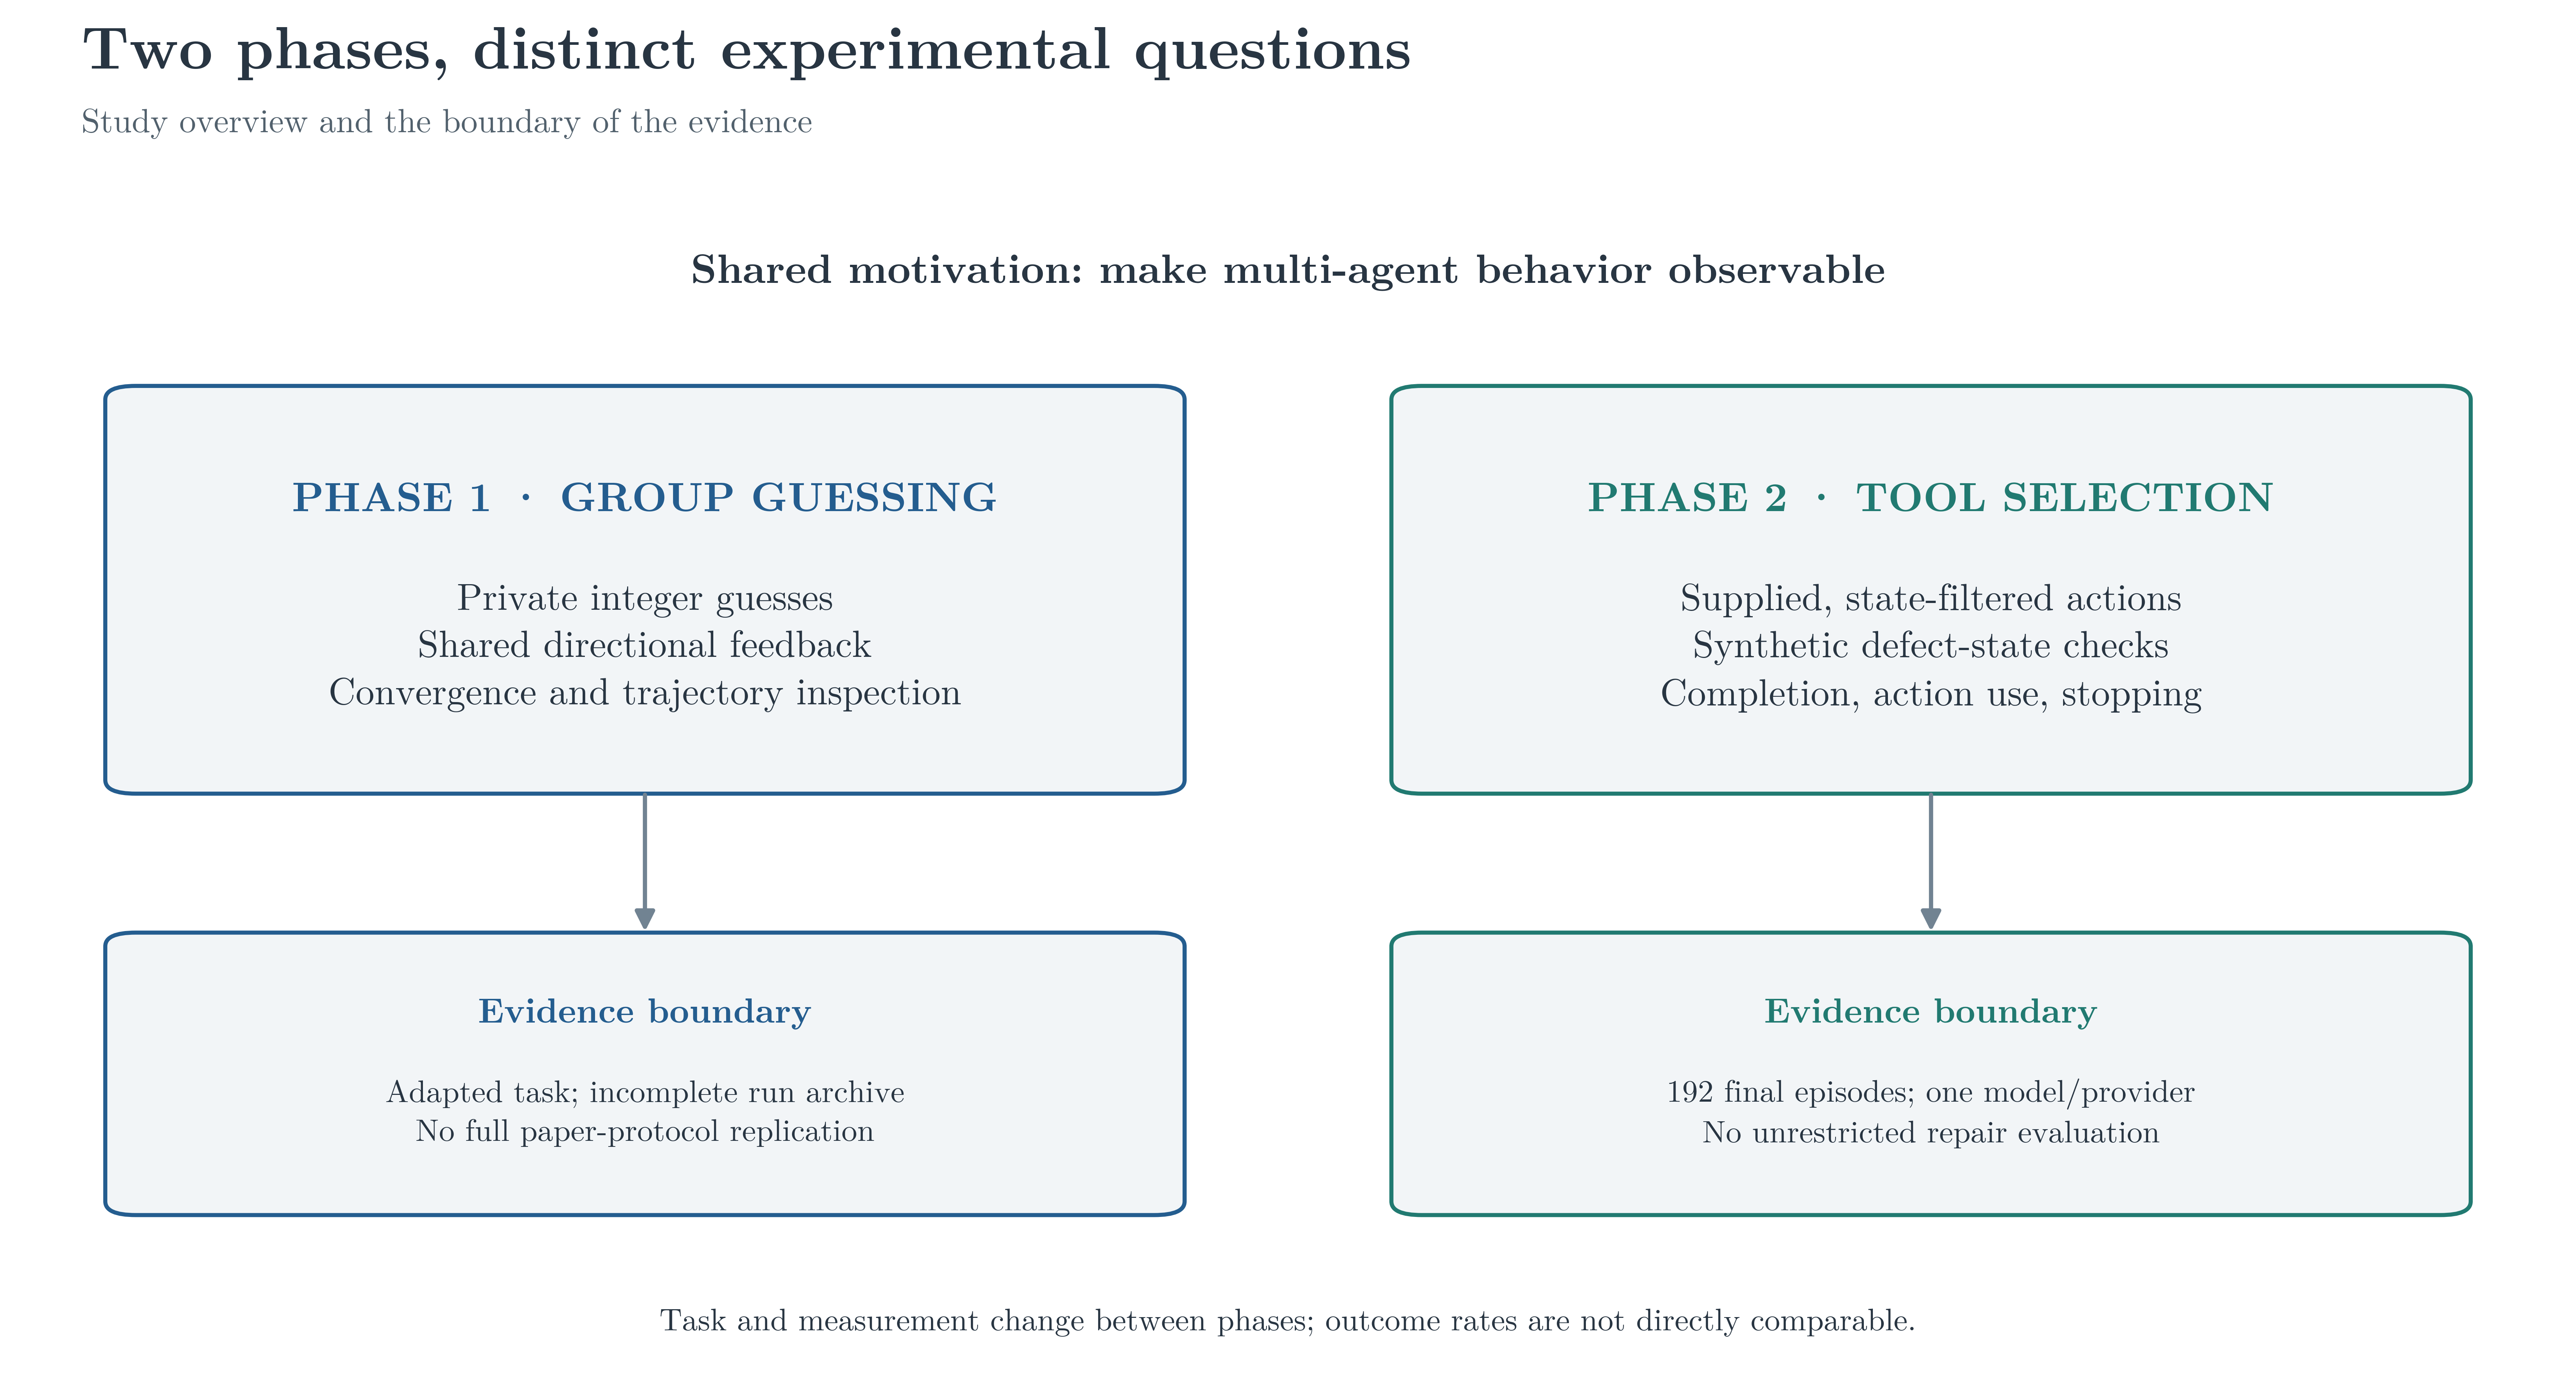
\includegraphics[width=\textwidth,height=0.68\textheight,keepaspectratio]{Images/01_two_phase_overview.png}
\caption{The two phases share a motivation but differ in task, observation unit, and analysis. The later Phase 1 action-wrapper bridge is an engineering validation, not a third experiment; it is described in Section 4.1.}
\label{figure:1}
\end{figure}
\subsection{Terminology for later chapters}
Use \textbf{paper emergence} only for the paper’s information-theoretic, temporal analyses; \textbf{synergy} and \textbf{redundancy} for PID components; \textbf{differentiation} for agent-specific contribution patterns; \textbf{alignment} for linkage to a shared task-relevant signal; and \textbf{complementarity} for differentiated contributions that are jointly useful. For Phase 2, use \textbf{categorical coordination estimate} or \textbf{action-profile mutual information}, not paper-style synergy or emergence. Keep \textbf{success}, \textbf{partial}, and \textbf{failure} as distinct episode outcomes.

\chapter{Phase 1: Historical Implementation}
\label{chapter-02}
\thispagestyle{plain}
\section{How the Phase 1 experiment took shape}
Phase 1 began with a repeated group-guessing task: each agent made a numerical contribution, the engine evaluated the group result, and the agents received shared directional feedback. As the implementation developed, the prompts were shaped to preserve each agent's own guess history without exposing peer guesses. A later persona branch added persona descriptions alongside instructions to reason about other agents; because these elements were introduced together, their separate effects cannot be identified. This progression established the private-contribution/shared-feedback protocol that motivates the bridge and the later tool-use study.

\section{Game and feedback loop}
The Phase 1 game engine (\texttt{experiment.py}) defines two aggregation modes. In \textbf{sum} mode, each agent is restricted to an integer from 0 through 50, and the hidden integer target is sampled uniformly from 51 through 100 by Python’s \texttt{random.randint}. The engine adds the current guesses and compares the total with that target. In \textbf{mean} mode, both target and individual-guess ranges default to 0 through 100; the engine computes the arithmetic mean of the agents’ guesses and applies Python’s \texttt{round} before comparing it with the integer target. The mode, ranges, sampled target, temperature, and round limit are recorded in the run configuration. These mechanics form a repository guessing task; they should not be read as evidence that the paper’s complete protocol or treatment design was implemented.

In either mode, feedback is categorical: \texttt{CORRECT!}, \texttt{too HIGH}, or \texttt{too LOW}. The numerical gap between the group value and target is not shown. A correct result ends the game immediately; otherwise, play continues until the configured maximum, normally 20 rounds in the runner settings. Thus the feedback tells agents the direction of error but not its size. The target is printed to the local console for the experiment operator, but the prompt sent to the agents does not include it.

The game manager retains a sequence of \texttt{Round} records. Each record contains agent-indexed guesses, the group result, feedback, target, mode, prompts, and response identifiers, with optional parsing/fallback markers. A notable naming detail is that \texttt{Round.average} stores the \textbf{sum} in sum mode and the unrounded mean in mean mode; \texttt{rounded\allowbreak\_average} stores the group value used for comparison (the sum or rounded mean). Interpretation therefore requires the mode field rather than assuming the field names have one invariant meaning.

\section{Private prompt histories}
Every \texttt{Agent} receives the shared round-history object, but \texttt{\allowbreak\_build\allowbreak\_strategic\allowbreak\_prompt} selects only \texttt{round\allowbreak\_data.guesses[self.agent\allowbreak\_id]} from each prior round. It pairs that private guess with the shared result label. The next prompt describes the game and the agent’s allowable range, lists its own earlier guesses and the repeated group feedback, then asks for a new integer. The first-round prompt instead states that the agent has not yet guessed and that no group feedback exists. Consequently, agents do not receive direct messages, peer identities, or the other agents’ guess values through this prompt. They can condition their later behavior on the common outcome while maintaining separate private guess histories.

The resulting signal is aggregate and lossy: it does not identify which teammate contributed to an overshoot or undershoot. The first guess is also model-generated. Prompts and round records were saved for selected inspection.

\section{Concurrent calls, parsing, and fallbacks}
Calls from agents in a round are concurrent; rounds proceed sequentially. Recovery is important when interpreting the results: the client can return a marked numeric fallback, while the parser can select, clamp, or substitute a number for malformed output. A recorded in-range guess is therefore not necessarily a direct model choice. As the implementation matured, parsing and response persistence were adjusted to make more of this recovery behavior visible.

\begin{figure}[htbp]
\centering
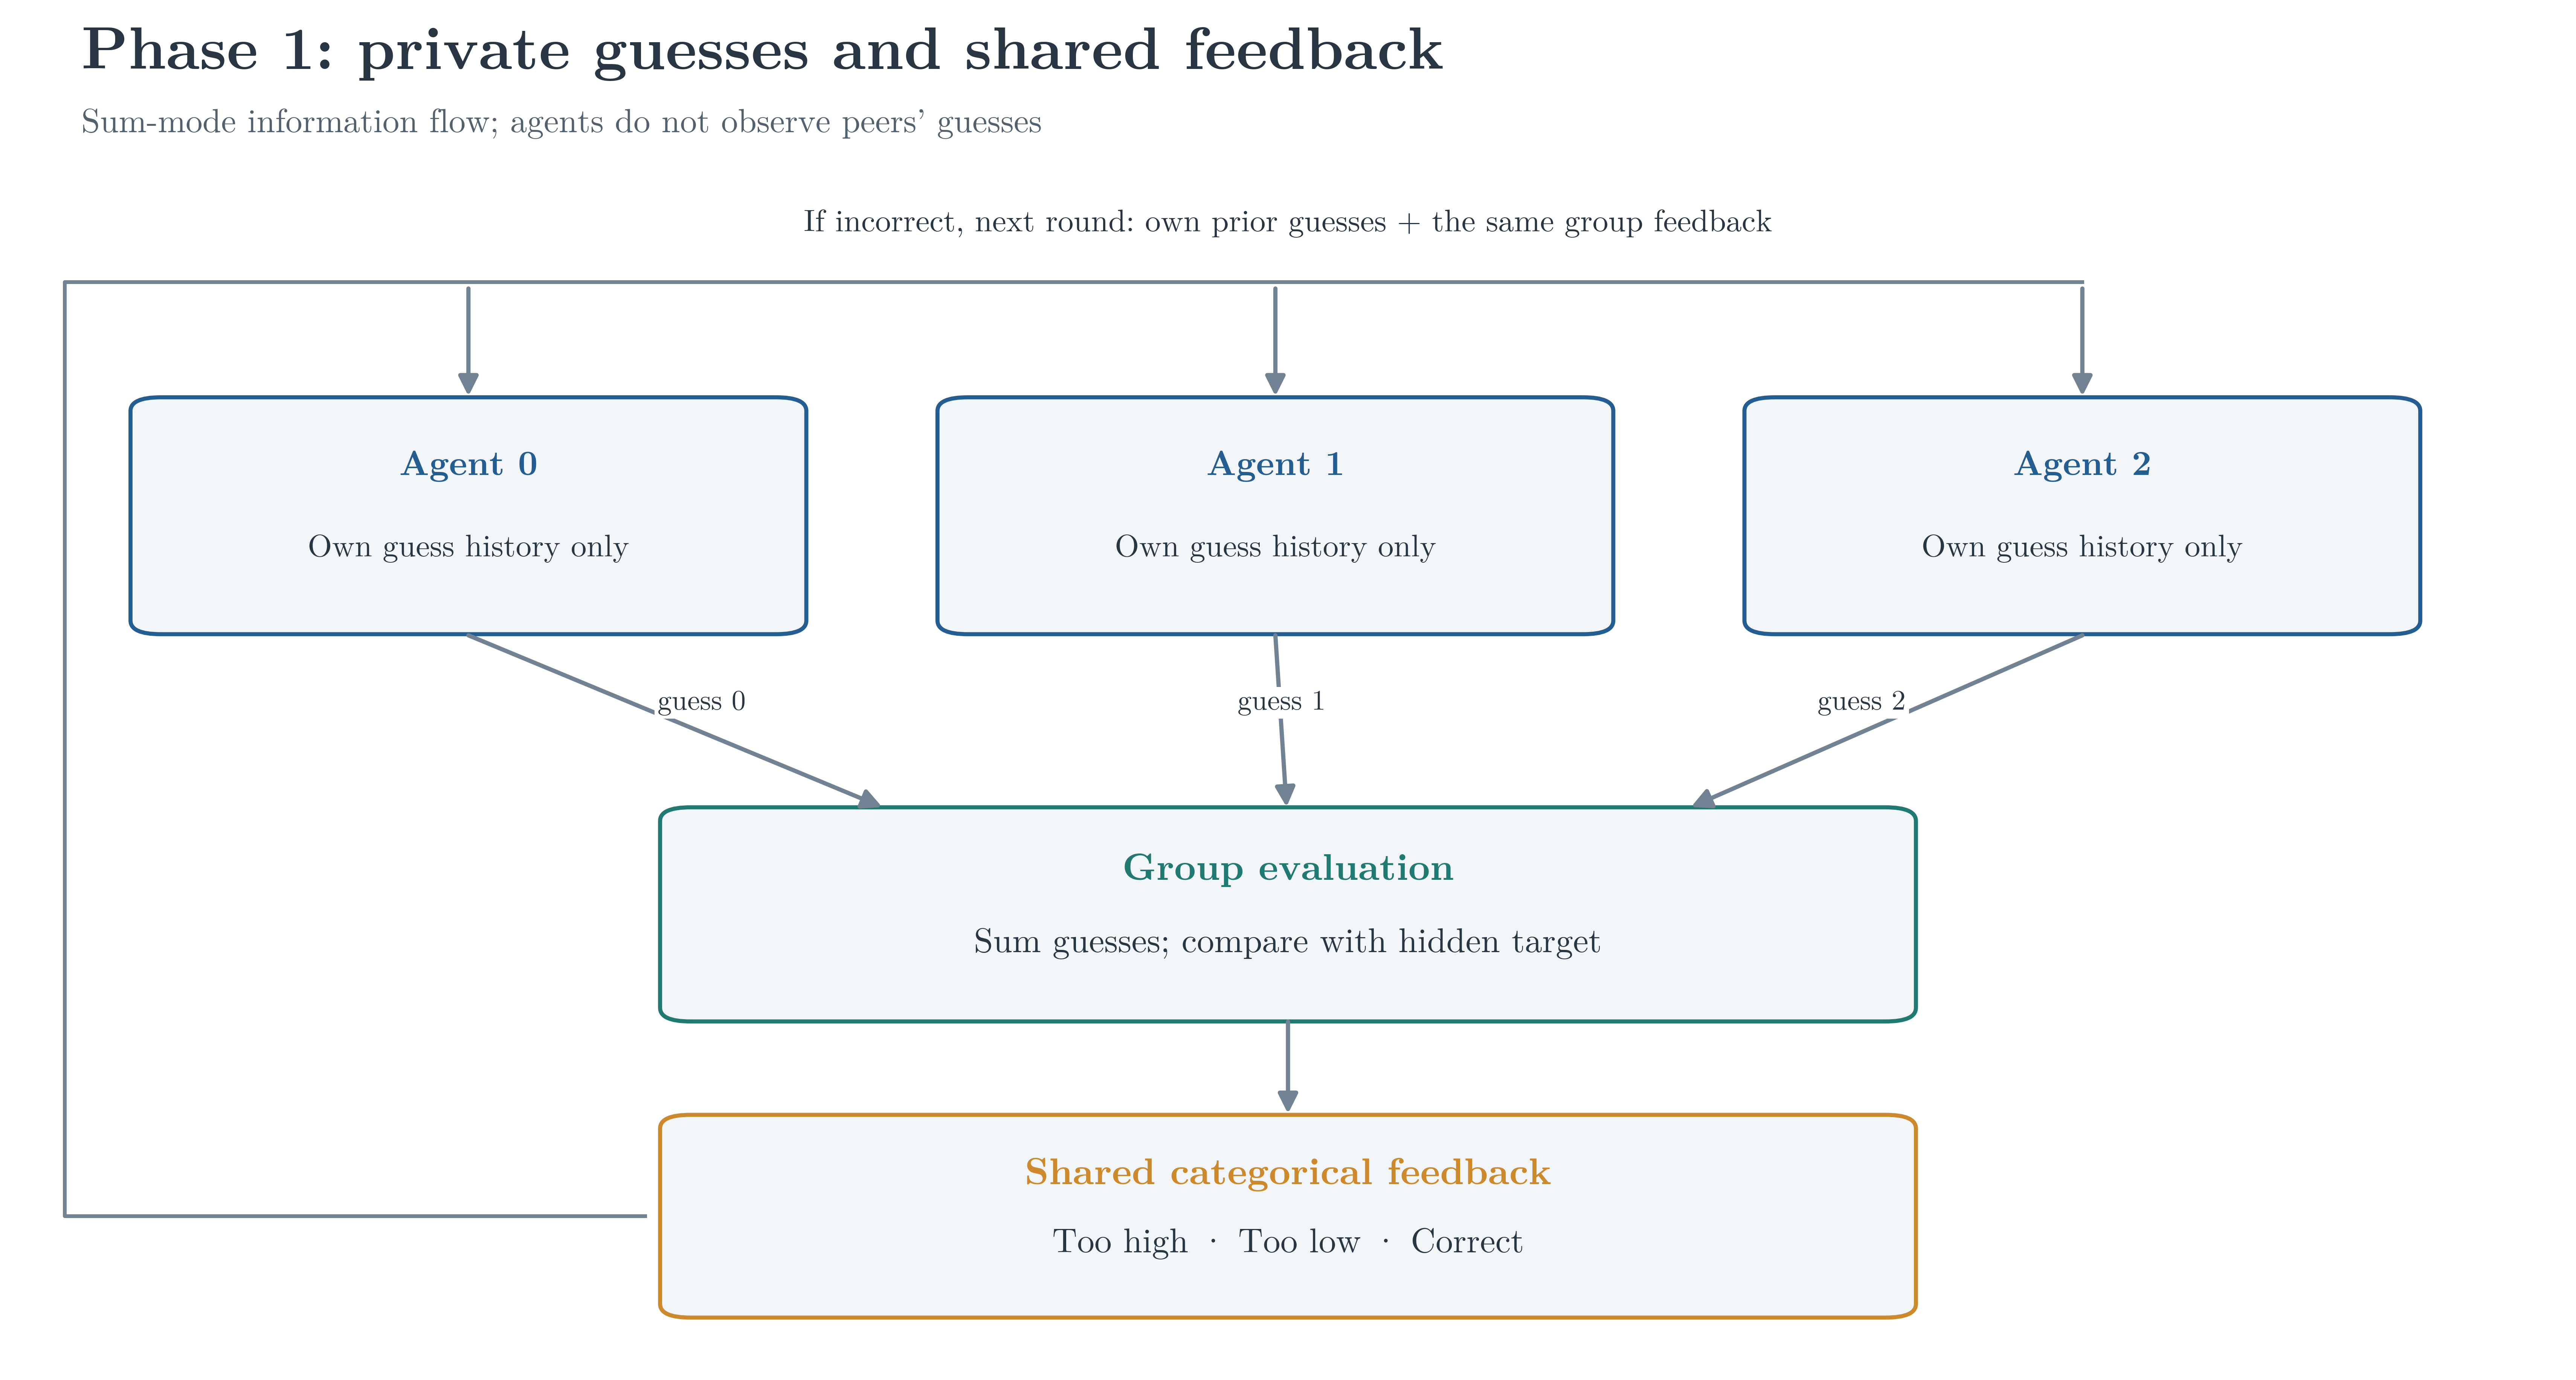
\includegraphics[width=\textwidth,height=0.68\textheight,keepaspectratio]{Images/02_phase1_feedback.png}
\caption{Illustrative three-agent sum-mode loop. Guesses are collected before group evaluation; agents retain their own guess histories and receive shared categorical feedback, not their peers’ guesses.}
\label{figure:2}
\end{figure}
\section{Persistence and parameter sweeps}
The runner saved round logs, prompt/response artifacts, configurations, and summaries. Its \texttt{completed\allowbreak\_successfully} field indicates that execution reached summary writing; \texttt{solved} separately indicates whether the target was reached. The configured sweep and a few curated trajectories are not evidence that the full advertised sweep completed.

\section{Persona branch}
The persona branch assigned shuffled persona text and also instructed agents to reason about others’ guesses and group progress. Because these prompt components were bundled, their effects cannot be separated; there was no matched Plain/Persona/ToM treatment matrix.

\section{Result analysis and limitations}
The historical analysis plotted convergence and rounds-to-solution from logs and exported selected trajectories, rather than a complete episode-level dataset or the paper’s information-theoretic analyses. Targets and persona order were not reproducibly seeded, and response recovery could affect recorded guesses.

\section{Transition to the maintained Phase 1 code}
As the project grew, the Phase 1 guessing-game code was kept in \texttt{base-paper/}, while the new tool-use work was developed in \texttt{baseline/}. This organization separated two tasks without changing the underlying question that connected them: how actions by multiple agents relate to a shared outcome.

\chapter{Phase 1: Maintained Base-Paper Implementation}
\label{chapter-03}
\thispagestyle{plain}
\section{Split and current scope}
The maintained Phase 1 game is in \texttt{base-paper/}; the later tool-use environment is in \texttt{baseline/}. This separation reflects a progression in experimental design, not a conversion of the guessing task into a bug-fixing task. Phase 1 remains a repository adaptation rather than the paper authors’ canonical implementation. The available saved trajectories are selected examples, not a complete run archive.

\section{Protocol and configured scope}
The maintained settings continue the same game and private-history protocol described in Sections 2.2–2.3. The current configuration describes three agents, six temperatures, and five repetitions (30 games per configured model), while the inherited README advertises a larger 3,990-run grid. Those are different statements of intended scope, not evidence that either complete sweep was run. The saved local example is one unsolved run, and \texttt{sampled\allowbreak\_data/} contains selected trajectories rather than a complete episode dataset.

\section{Changes that affect interpretation}
The persona path combines shuffled persona text with instructions to reason about other agents and the group objective. There is no matched Plain/Persona/ToM treatment matrix, so the persona and reasoning effects cannot be separated.

Later maintenance made some failures more visible: exhausted number extraction raises a parsing error, and round records preserve additional response/fallback information. The base agent can still reuse a previous guess or substitute a midpoint; the API client can still return a numeric fallback, and the parser can select or clamp numbers from malformed text. Consequently, an in-range action is not necessarily an unaltered model choice. The persona path has a different parsing and error-handling path.

The saved local example records its own model, settings, target, and outcome; it does not match current defaults. Read run artifacts together with their saved configuration, and do not infer completion from a configured sweep or a successful execution status alone (\texttt{completed\allowbreak\_successfully} is distinct from \texttt{solved}).

\section{Boundary of the evidence}
Targets and persona assignment were not reproducibly seeded in the historical path, and the available sample does not establish a completed sweep. The repository does not contain the paper’s complete intervention matrix or time-delayed information-theoretic analysis. These limitations mean Phase 1 should be understood as a repository adaptation, not a complete replication.

The bridge uses the maintained game rules and settings represented by \texttt{experiment.py} and \texttt{settings.py}. Its historical reference is the saved Phase 1 run, whose configuration records five \texttt{openai/gpt-4o-mini} agents, sum mode, temperature 1, target 57 in range 51–100, guesses in range 0–50, and a 20-round limit. Because the saved trajectory does not describe every implementation detail from the time it was generated, the bridge treats its recorded rounds as the reference and checks their already-parsed guesses against the maintained rules. It does not reconstruct the original model responses or prompting.

\chapter{Phase 2: Motivation and Tool-Call Expansion Plan}
\label{chapter-04}
\thispagestyle{plain}
\section{Why change the task?}
Phase 1 records numerical contributions made under private histories and shared, coarse directional feedback; its original experiment does not expose a distinct tool operation or explicit intermediate task state. Phase 2 changed the unit of observation to explicit actions against a controlled task state, recording action type, arguments, state transitions, and outcomes. A later bridge now represents the same Phase 1 contribution as \texttt{submit\allowbreak\_guess(value)} and records its actor, without changing the original experiment.

This was a methodological extension, not a correction to the guessing game or a direct reproduction of its paper. Its purpose was to improve control and observability for a different task. The bridge is a later engineering validation, completed after the Phase 2 experiments and final run; it was not part of Phase 2's original design or evidence available when those runs were conducted.

\begin{table}[htbp]
\centering
\small
\setlength{\tabcolsep}{4pt}
\begin{tabularx}{\linewidth}{|Y|Y|Y|Y|}
\hline
\textbf{Dimension} & \textbf{Phase 1 guessing game} & \textbf{Later Phase 1 bridge} & \textbf{Phase 2 tool-use experiment} \\
\hline
Action representation & One numerical guess per agent and round & \texttt{submit\allowbreak\_guess(value)} with \texttt{agent\allowbreak\_id} event metadata and a numerical-contribution category & Select among supplied retrieval, update, verification, and finalization actions \\
\hline
Agent-visible state & Private own-guess history and shared directional feedback; no peer guesses, target, or group size & Preserves those observation restrictions and withholds new feedback until all round contributions arrive & Explicit intermediate task state is shared across sequential turns and nominal actor IDs \\
\hline
Evaluation and stopping & Configured sum or rounded mean; solved or unsolved at the round limit & Reuses those rules; execution completion is recorded separately from the native solved/unsolved outcome & Synthetic fixture rules produce success, partial, or failure; the tool-call budget is separate from Phase 1 rounds \\
\hline
Trace & Per-round guesses and aggregate feedback & Actor/action events linked to per-round aggregates, feedback, and terminal outcome & State-changing tool events linked to episode outcome \\
\hline
\end{tabularx}
\caption{Comparison of the three project stages}
\end{table}
\subsection{Later bridge-validation check}
The offline runner compared the one available historical trajectory—five agents, sum mode, target 57, 20 rounds, unsolved—with its saved per-round JSON. It checked each agent's recorded contribution and identity, the legacy \texttt{average} and \texttt{rounded\allowbreak\_average} fields, the comparison value, feedback, round count, and stopping outcome. All 20 historical rounds matched with zero mismatches. The repository has no saved mean-mode or solved Phase 1 trajectory, so a clearly labeled synthetic regression case checked mean rounding at 0.5 and 1.5, feedback, and solved early stopping in two rounds; it also matched with zero mismatches. The output records one historical trajectory, one synthetic case, 22 total rounds, 104 submitted actions, and both configurations in replay\allowbreak\_report.json. The saved \texttt{average} field is a sum in sum mode and an unrounded arithmetic mean in mean mode; \texttt{rounded\allowbreak\_average} is the comparison value in either mode.

Seven focused Phase 1 wrapper tests and six existing Phase 2 environment tests passed. The historical replay and synthetic regression are separate bridge cases; they are not added to Phase 2's 192 episodes or 1,181 tool events. This validates environment transitions for supplied, already-parsed actions only—not model responses, prompts, parsing, the original paper's findings, emergence, PID synergy, autonomous-agent collaboration, or improved coordination. It establishes framework continuity, not equivalence of the two experiments.

\section{A controlled synthetic bug-fix workflow}
Synthetic bug fixing was selected for Phase 2 because it supports a finite catalog of task instances, constrained operations, and outcomes that can be evaluated by the environment. The fixture builder defines eight templates with two variants each, for 16 variants; some variants include an additional required defect. The environment gives agents access to five tools: \texttt{retrieve\allowbreak\_file}, \texttt{search\allowbreak\_symbol}, \texttt{run\allowbreak\_tests}, \texttt{apply\allowbreak\_patch}, and \texttt{finalize\allowbreak\_ticket} (baseline/plan.md; baseline/tool\allowbreak\_use\allowbreak\_environment.py; baseline/settings.py).

Each fixture specifies the files, symbols, defects, requirements, and checks relevant to its task. Tool calls are validated against their argument schemas and the current state. A valid patch can alter the simulated task state; retrieval and symbol search expose fixture information; test calls assess the fixture’s declared conditions; finalization ends the task under the environment’s outcome rules. The environment records progress and classifies a completed episode as \texttt{success}, \texttt{partial}, or \texttt{failure}. Its state and step-budget checks allow invalid calls to be categorized rather than silently blended into ordinary progress. These mechanics replace one scalar shared response with a sequence of explicit state-mediated actions.

This action-oriented design sits alongside prior work that treats model behavior as tool-mediated trajectories. ReAct interleaves reasoning with actions in external environments, while API-Bank evaluates planning, retrieval, and API calls (Yao et al., 2023; Li, M. et al., 2023). Frameworks such as AutoGen and CAMEL explore configurable or role-based conversations among language-model agents (Wu et al., 2023; Li, G. et al., 2023), and the LLM-Coordination benchmark studies agent decisions in pure coordination games (Agashe et al., 2023). Surveys organize this broader work around collaboration mechanisms and the progression from single calls to multi-tool orchestration with intermediate state and feedback (Tran et al., 2025; Xu et al., 2026). The present task differs from those settings: its actions are selected from a fixture-specific allow-list, its state transitions are deterministic, and its multi-agent policies use sequential turns in shared context. These works provide context for explicit action traces and coordination questions; they do not make this experiment equivalent to those systems or establish a field-wide novelty claim.

The meaning of fixture-based checking is specified with the implemented evaluator in Section 5.1; it should not be confused with validating a repair in a real repository.

Explicit transitions distinguish information gathering from patching, record patch acceptance, and expose redundant, invalid, or out-of-budget calls. Linking these events to outcomes improves control and traceability; it does not show that tool use is inherently more coordinated or capable.

\section{Policy comparisons and the role of abstraction}
The first policy layer was scripted, so the environment and analysis pipeline could be exercised without conflating every result with a model response. The four scripted conditions are \texttt{single\allowbreak\_agent}, \texttt{random\allowbreak\_policy}, \texttt{independent\allowbreak\_multi\allowbreak\_agent}, and \texttt{prompted\allowbreak\_coordination}. They provide a one-agent reference, valid-action exploration, independent multi-agent behavior, and a scripted shared coordination plan. The label \texttt{prompted\allowbreak\_coordination} in this scripted set does not mean an LLM received a prompt intervention. These policies take sequential turns against shared state; unlike Phase 1’s concurrent calls within a round, they are not simultaneous actions (baseline/tool\allowbreak\_use\allowbreak\_baselines.py).

Model-backed counterparts later added \texttt{llm\allowbreak\_single\allowbreak\_agent}, \texttt{llm\allowbreak\_independent\allowbreak\_multi\allowbreak\_agent}, and \texttt{llm\allowbreak\_prompted\allowbreak\_coordination}. The adapter requests a valid structured action and records parsing/retry behavior, errors, and fallbacks. These conditions compare one-agent and multi-agent workflows and independent versus coordination-oriented instructions, but do not isolate every causal mechanism or recreate the paper’s Plain/Persona/theory-of-mind matrix. They also depend on an external service. Persona studies were outside the initial tool-use scope (baseline/plan.md; baseline/tool\allowbreak\_use\allowbreak\_baselines.py; baseline/llm\allowbreak\_client.py).

Raw action sequences are informative but can be too sparse or high-cardinality for stable categorical estimation. The design therefore proposed an abstraction from individual tool events to categories: \texttt{retrieve}, \texttt{verify}, \texttt{update}, \texttt{finalize}, and \texttt{error\allowbreak\_or\allowbreak\_noop}. The current analysis derives bounded per-agent action counts and a \texttt{coarsened\allowbreak\_action\allowbreak\_profile} from those categories, while retaining alternate representations for comparison. The profile reduces the number of distinct joint states compared with a full trace in the scripted pilot. It is a tractable representation for categorical analysis, not a validated human interpretation of what each trajectory means. Human labeling and inter-rater agreement were part of the proposed abstraction-validation protocol, but were not completed in the evidence reviewed for this chapter (baseline/coordination\allowbreak\_analysis.py; baseline/validation.md).

\section{From trace logging to outcome-linked measurement}
The planned trajectory schema aimed to preserve event order, actor, tool, arguments, outputs, state/progress information, invalid-call diagnostics, and episode outcome. The implemented pipeline writes a canonical \texttt{episode.jsonl} event stream alongside \texttt{summary.json} and \texttt{task\allowbreak\_fixture.json}; sweep outputs add configuration, progress, aggregate summaries, and a manifest. This provides a clearer audit path from a fixture and policy to the actions taken and the environment’s final classification. Trajectory exporters produce event- and episode-level tables for downstream analysis (baseline/plan.md; baseline/context\allowbreak\_methods.md; baseline/export\allowbreak\_trajectory\allowbreak\_data.py; baseline/run\allowbreak\_baseline\allowbreak\_sweep.py).

The planned primary coordination statistic was categorical mutual information between a pair of agent action representations and the ternary episode outcome, written as \$I(A\allowbreak\_1,A\allowbreak\_2;Y)\$. In the implemented report, eligible two-agent episodes contribute joint action-profile categories and outcomes; single-agent episodes are presented as a separate reference and are excluded from the two-agent estimate. Smoothing sensitivity, bootstrap intervals, and permutation nulls add diagnostics around the estimate. This links observed action patterns to an outcome label more directly than raw convergence counts do, but it is still an association over categorical summaries. With small samples, sparse joint states, or nearly constant outcomes, the estimate can be unstable or uninformative. A nonzero value does not establish that a policy caused success or that a collective property emerged.

This measure is also not the paper’s temporal mutual information or partial information decomposition. Phase 2 does not thereby measure paper-style synergy, redundancy, differentiation, or complementarity. Its contribution is a more explicit and auditable action-to-outcome analysis in a new task, not replication of the paper’s empirical claims.

\section{Validation goals and eventual status}
The initial validation plan was broader than “the scripts run.” It called for unit checks of state transitions, invalid calls, policies, and terminal outcomes; schema and ordering checks for event/export files; assertions that abstraction categories cover events; a stratified human-labeling exercise with adjudication and Cohen’s kappa; categorical-MI sanity cases; and an end-to-end fixed-seed pilot of 200–400 episodes. Sanity cases were intended to test expected behavior under independent, shuffled, duplicated, and complementary scripted traces, and to check estimator uncertainty and sensitivity to sample size and category count (baseline/plan.md; baseline/validation.md).

The implementation developed alongside the research question. The maintained guessing game was kept in \texttt{base-paper/}, and a separate \texttt{baseline/} environment was built around explicit state-changing actions. Scripted policies first exercised that environment and its analysis pipeline; model-backed policies were added for the pilot and final collection. Later maintenance strengthened manifest handling, retry records, audit checks, and resumption. These stages explain how the project moved from a compact aggregate-feedback task toward a more observable tool-use framework. They should not be read as a single unchanged implementation or as evidence that later safeguards were present in earlier runs.

The implementation advanced beyond the first tracker. The final model-backed run contains 192 completed summaries; its export manifest records 192 episodes and 1,181 events with no issues (final progress; export manifest). The run also retains fixture/configuration records, coordination output, and quality-control documentation. The active \texttt{baseline/tests/} suite passed 61 tests from the project root. The tracker marks the lower-cardinality profile and MI sanity suite complete. These establish software and pipeline validation, not methodological validation of every estimate or conclusion.

The Phase 2 evidence did not establish the planned human-rating/adjudication study, cross-metric correlation analysis, deterministic replay of identical Phase 2 trajectories, or comprehensive full-dataset schema and semantic audits. The Phase 1 wrapper received a narrow saved-guess replay (Section 4.1); this does not validate Phase 2 trajectories. The targeted Phase 2 audit reported in Section 9.6 checked identity, counts, event ordering, and hash consistency, but not comprehensive schema, semantic, or replay validation. Fixed assignments, manifests, seeds, and resumability support design reproducibility and artifact recovery, but cannot make LLM outputs deterministic. The tracker’s 80-episode event count is stale (558); pilot artifacts support 546. Its 200–400 target was for an early scripted pilot, not the final LLM dataset, which contains 192 episodes under a different design.

As specified for this project, scope was mentor-guided and time-limited. Work prioritized controlled fixtures, explicit actions, scripted and model-backed pipelines, and descriptive outcome-linked measurement. Human validation, correlation analysis, persona studies, and paper-style PID/synergy were omitted or deferred, not achieved. Repository records establish these boundaries but not which individual choice a mentor directed. Scripted policies were implemented and piloted; they were not wholly deferred.

\section{Plan and implementation}
\begin{table}[htbp]
\centering
\small
\setlength{\tabcolsep}{4pt}
\begin{tabularx}{\linewidth}{|Y|Y|Y|}
\hline
\textbf{Dimension} & \textbf{Planned direction} & \textbf{Implemented and evidenced status} \\
\hline
Task and control & Deterministic bug-fix fixtures, explicit tools, validated state transitions, and ternary terminal outcomes & Implemented in the fixture environment; tests cover transitions and invalid calls. Checks are synthetic fixture evaluations, not real code execution. \\
\hline
Policies & Single-agent, random-valid, independent multi-agent, and prompted coordination; later model-backed counterparts & Four scripted policies were implemented and used in the 80-episode pilot; three LLM-backed conditions were added and used in the separate final run. Turns are sequential over shared state. \\
\hline
Trajectories & Canonical event stream plus tabular/columnar export, with event and state details & JSONL episode events, summaries, fixtures, manifests, CSV/Parquet exports, and an export manifest exist. Final-run export reports 192 episodes and 1,181 events with no issues. \\
\hline
Action abstraction & Mutually exclusive/exhaustive action categories, then lower-cardinality features for MI & Category-based count/profile analysis and MI sanity tests were implemented. Full-dataset coverage, human labeling, adjudication, and inter-rater reliability remain unverified. \\
\hline
Outcome-linked analysis & Categorical \$I(A\allowbreak\_1,A\allowbreak\_2;Y)\$ with uncertainty, null checks, and checks for estimator behavior & Bootstrap/permutation reporting and the sanity suite are implemented. Interpretation remains constrained by sample size, state cardinality, and outcome distributions; this is not paper-style PID/TDMI. \\
\hline
Validation and scale & Schema/replay checks and a 200–400 episode scripted pilot, followed by reproducibility checks & The final LLM run completed 192 episodes; the baseline test suite and saved exports/QC were reported. Targeted identity/count/order/hash-consistency checks are reported in Section 9.6. The later Phase 1 bridge checks are reported separately in Section 4.1. Comprehensive Phase 2 schema and semantic audits, deterministic replay, human validation, and correlation analyses remain incomplete. \\
\hline
\end{tabularx}
\caption{Planned and completed Phase 2 work}
\end{table}
The expansion thus addressed Phase 1’s measurable limits by making the action sequence, task state, and outcome more explicit and machine-checkable. The result is a stronger basis for control, auditing, and replay-oriented analysis, with remaining validation needs clearly bounded. It is not evidence of superiority over Phase 1 agents, nor a replication of the paper’s findings.

\chapter{Phase 2: Implemented Architecture}
\label{chapter-05}
\thispagestyle{plain}
\section{Execution model and deterministic task catalog}
The active Phase 2 path begins with a catalog of synthetic bug-fix tasks, not a live repository. \texttt{build\allowbreak\_bugfix\allowbreak\_task\allowbreak\_fixtures()} in tool\allowbreak\_use\allowbreak\_environment.py constructs eight task templates with two named variants each, for 16 fixture variants. Each variant contains a title and description, in-memory source and placeholder test files, symbol references, a catalog of recognized patches, test-target specifications, and required defect identifiers. The two harder variants add a third required defect. A patch specification links an exact old text and replacement to the defect it fixes; the environment does not accept arbitrary patch content as a successful change.

Runtime settings are centralized in settings.py. They identify \texttt{synthetic\allowbreak\_bugfix}, the configured policy names, agent count, step budget, repetitions or seed list, batch size, result prefix, and LLM defaults. The thesis configuration uses three LLM-backed policies, two agents for multi-agent conditions, a 12-call step budget, four repetitions per fixture, seed start 200, and strict LLM mode. \texttt{run\allowbreak\_baseline\allowbreak\_sweep.py} turns these settings into a run configuration and a concrete manifest before episode execution. Single-agent policy names override the configured agent count to one.

\texttt{ToolUseBugfixEnvironment} holds the mutable episode state. It begins at \texttt{not\allowbreak\_started} with a deep copy of fixture files, zero steps, and empty collections for observed files and symbols, executed tests, applied patch IDs, fixed defects, and active regressions. Valid task progress changes the state to \texttt{in\allowbreak\_progress}. A terminal outcome maps to \texttt{completed\allowbreak\_success}, \texttt{completed\allowbreak\_partial}, or \texttt{completed\allowbreak\_failure}. Each environment instance also records its seed, fixture identity, event sequence, invalid-call counters, schema and environment versions, and a short configuration hash derived from the environment version, fixture, seed, agent count, and step budget.

An episode ends when a policy finalizes, or when its step budget is exhausted. \texttt{success} requires all required defects fixed and every fixture test target to pass without a disallowed regression. \texttt{partial} requires some required defect progress, incomplete tests, and no catastrophic regression. Otherwise the outcome is \texttt{failure}. Budget exhaustion invokes the same outcome logic without requiring an explicit finalization call. These labels are task outcomes computed from fixture state; they are not judgments about whether real software was repaired. In particular, generated test files contain placeholder assertions, and \texttt{run\allowbreak\_tests} checks defect identifiers and regression guards in the environment state. It does not execute pytest, run patched code, or access a real project.

\begin{figure}[htbp]
\centering
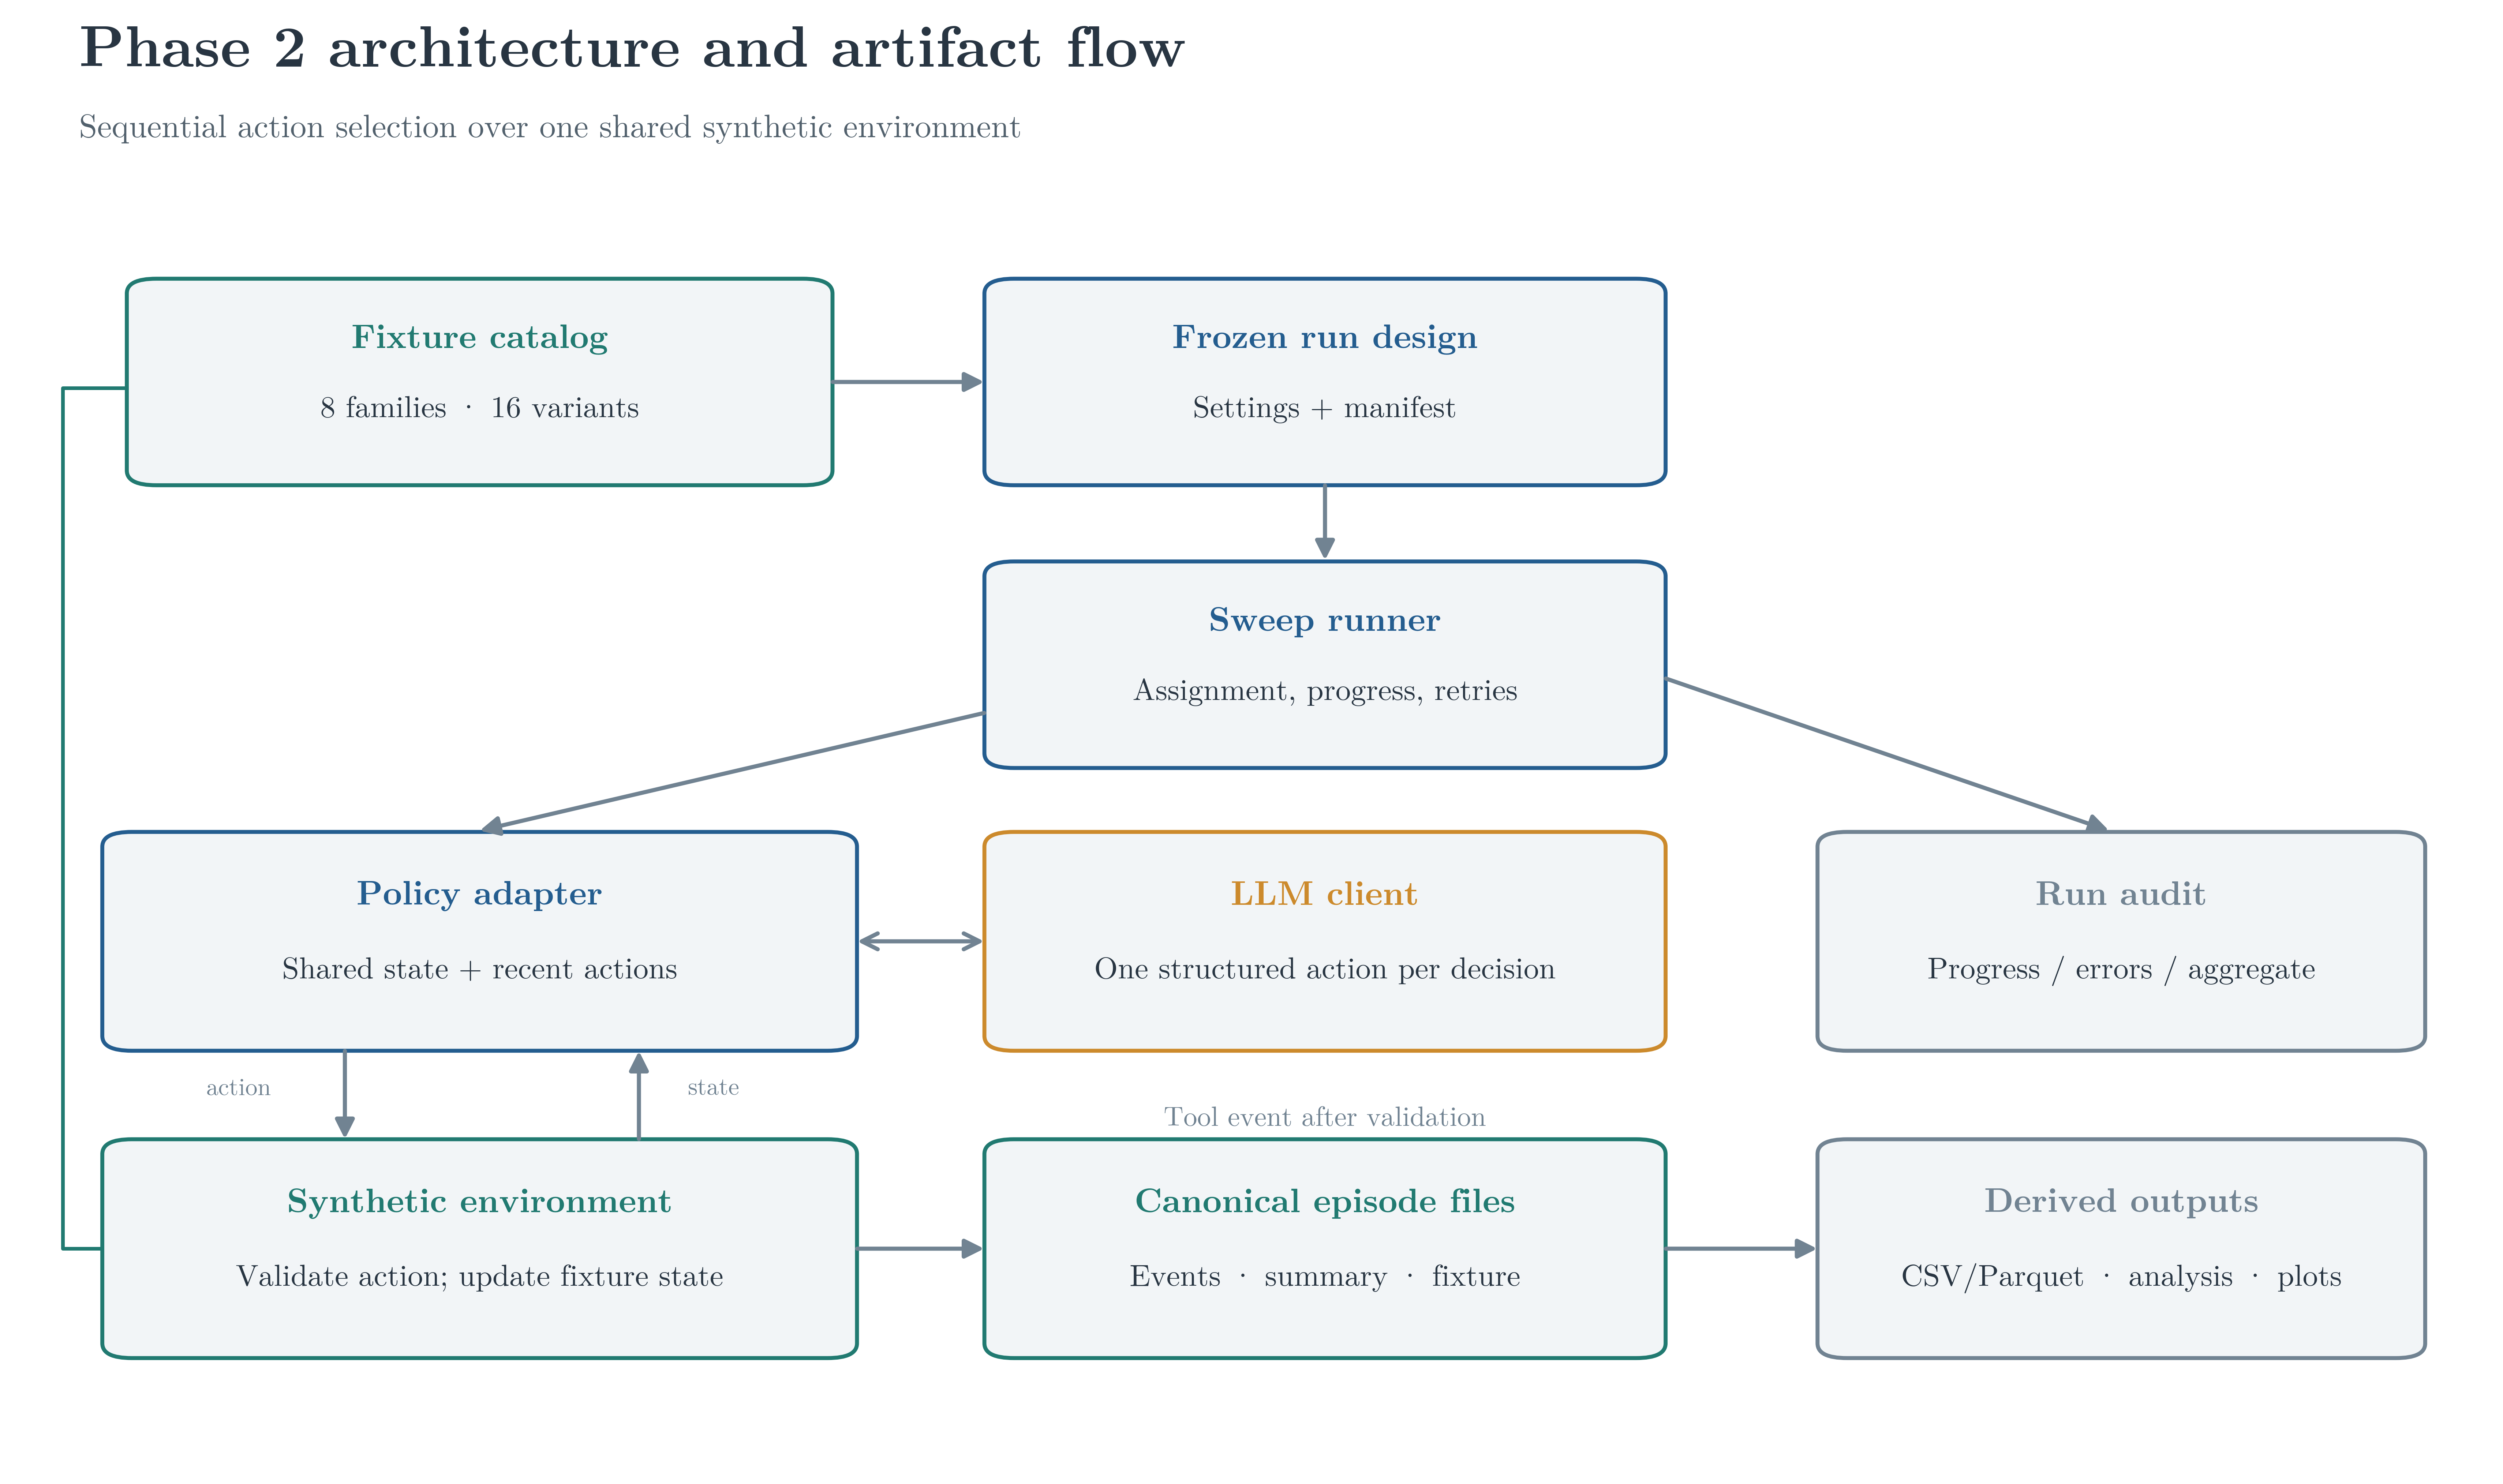
\includegraphics[width=\textwidth,height=0.68\textheight,keepaspectratio]{Images/03_phase2_architecture.png}
\caption{Phase 2 pipeline from fixture catalog and run design through policy selection, environment validation, canonical episode records, audit, and derived outputs. Nominal actor IDs share one sequential context.}
\label{figure:3}
\end{figure}
\begin{figure}[htbp]
\centering
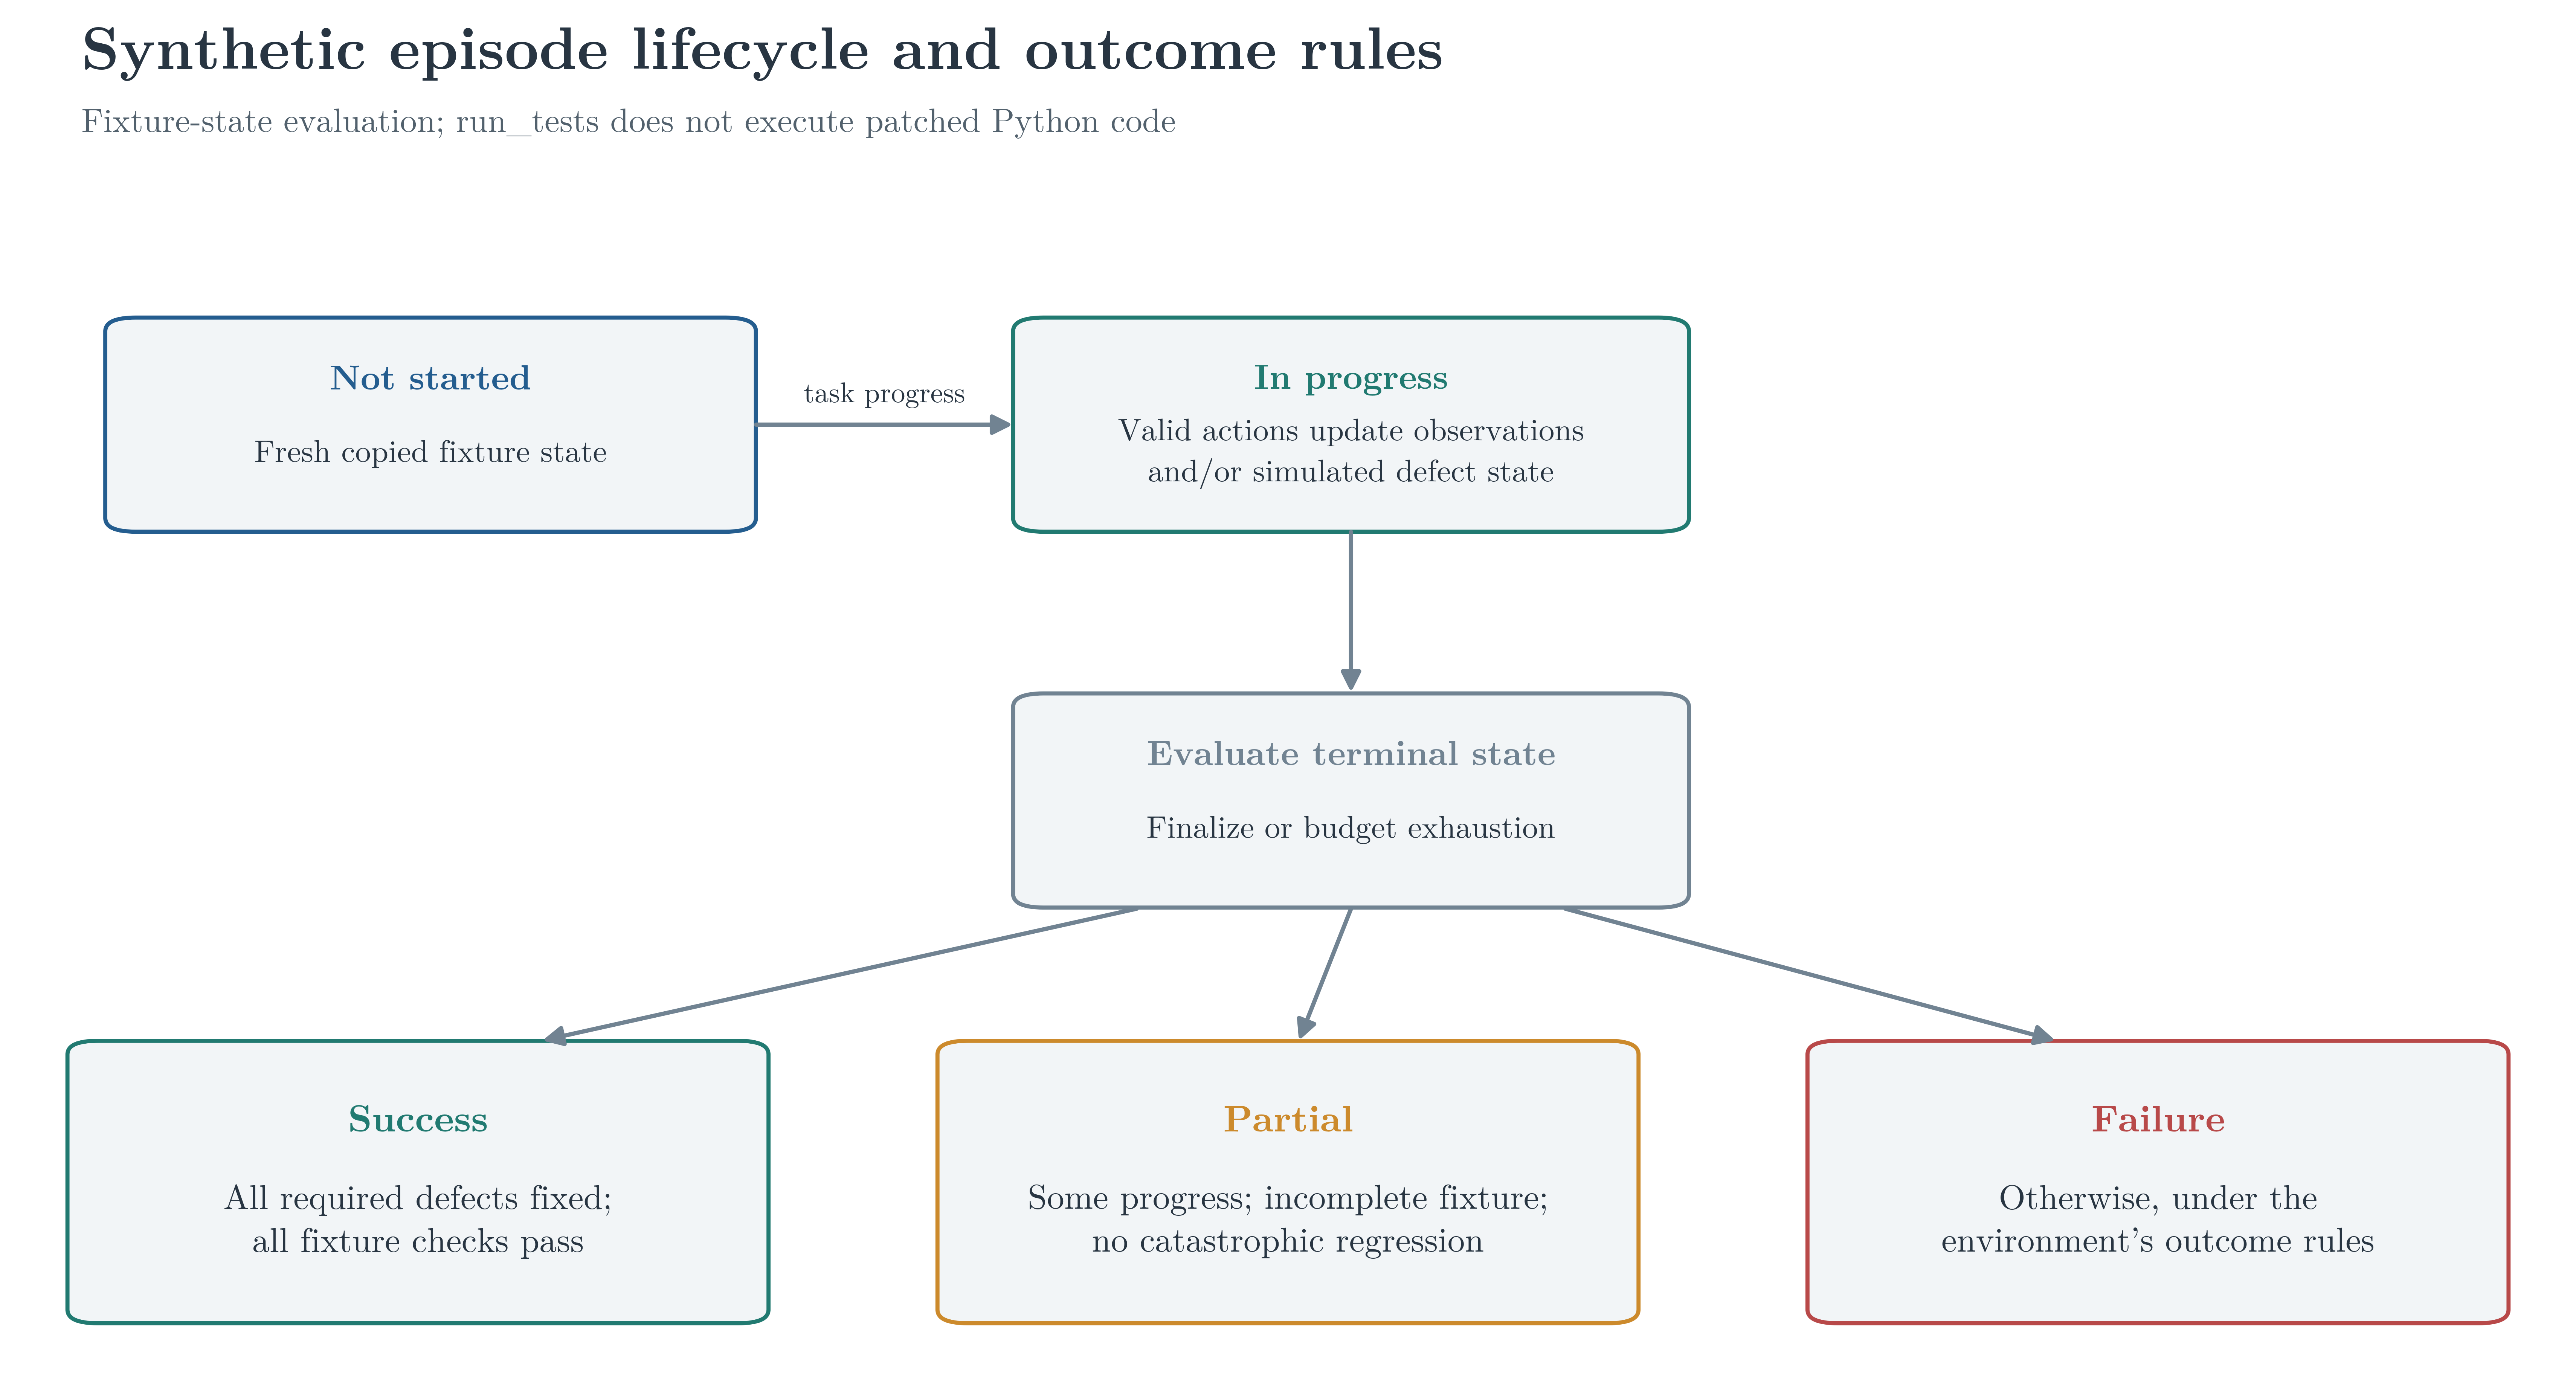
\includegraphics[width=\textwidth,height=0.68\textheight,keepaspectratio]{Images/18_episode_lifecycle.png}
\caption{Synthetic fixture state advances through valid actions and is classified at finalization or budget exhaustion. These are environment outcomes, not evidence that patched software was executed or repaired.}
\label{figure:4}
\end{figure}
\section{Tool contract, validation, and state transitions}
The environment exposes five tool names: \texttt{retrieve\allowbreak\_file}, \texttt{search\allowbreak\_symbol}, \texttt{run\allowbreak\_tests}, \texttt{apply\allowbreak\_patch}, and \texttt{finalize\allowbreak\_ticket}. \texttt{list\allowbreak\_valid\allowbreak\_actions()} enumerates actions available in the current state and budget, including known paths, symbols, test targets, and unapplied patches whose old context remains present. Finalization is offered after an update or test action. It returns no actions once the environment is terminal or the step budget is spent. LLM prompts use this current list as an allow-list; environment handlers independently validate each submitted call.

Each tool has a strict argument shape at the environment boundary. Retrieval requires a string \texttt{path} and optionally accepts a \texttt{span} object with exactly integer \texttt{start} and \texttt{end} keys. Symbol search requires a string \texttt{name}. Test execution takes no arguments or an optional string \texttt{test\allowbreak\_target}. Patch application requires a string \texttt{patch}; finalization requires a nonempty string \texttt{reason}. Extra keys, absent required keys, and wrong types are rejected. After schema validation, the environment checks whether referenced files, symbols, test targets, patch specifications, and patch context exist. A recognized patch is applied once and updates fixed-defect state; tests report which required defects remain; finalization classifies the current state.

The invalid-call taxonomy distinguishes five mechanisms rather than collapsing all failures: \texttt{schema\allowbreak\_invalid} for malformed arguments or unknown tool names; \texttt{reference\allowbreak\_invalid} for unknown paths, symbols, tests, or patch/context references; \texttt{state\allowbreak\_invalid} for an operation that is disallowed in the current episode state, such as finalizing before any update or verification; \texttt{semantic\allowbreak\_noop} for empty, already-applied, or non-changing patches; and \texttt{budget\allowbreak\_invalid} for calls made after the step budget is exhausted. Calls after terminal completion are state-invalid. Invalid attempts are emitted as events with an \texttt{error\allowbreak\_or\allowbreak\_noop} abstraction and increment the relevant counter. The episode summary's invalid-call rate is total invalid calls divided by environment step count; it is distinct from model-response parse errors, which may be recovered before the environment receives an action.

Retrieval and symbol search record observations; patches mutate simulated files and defect sets; tests record results; finalization sets the outcome. Environment tests cover transitions, invalid early finalization, required fixes, budget partials, repeated-patch no-ops, and the hard fixture (test\allowbreak\_tool\allowbreak\_use\allowbreak\_environment.py). Policy tests cover finalization gating and scripted outcomes (test\allowbreak\_tool\allowbreak\_use\allowbreak\_baselines.py).

\begin{figure}[htbp]
\centering
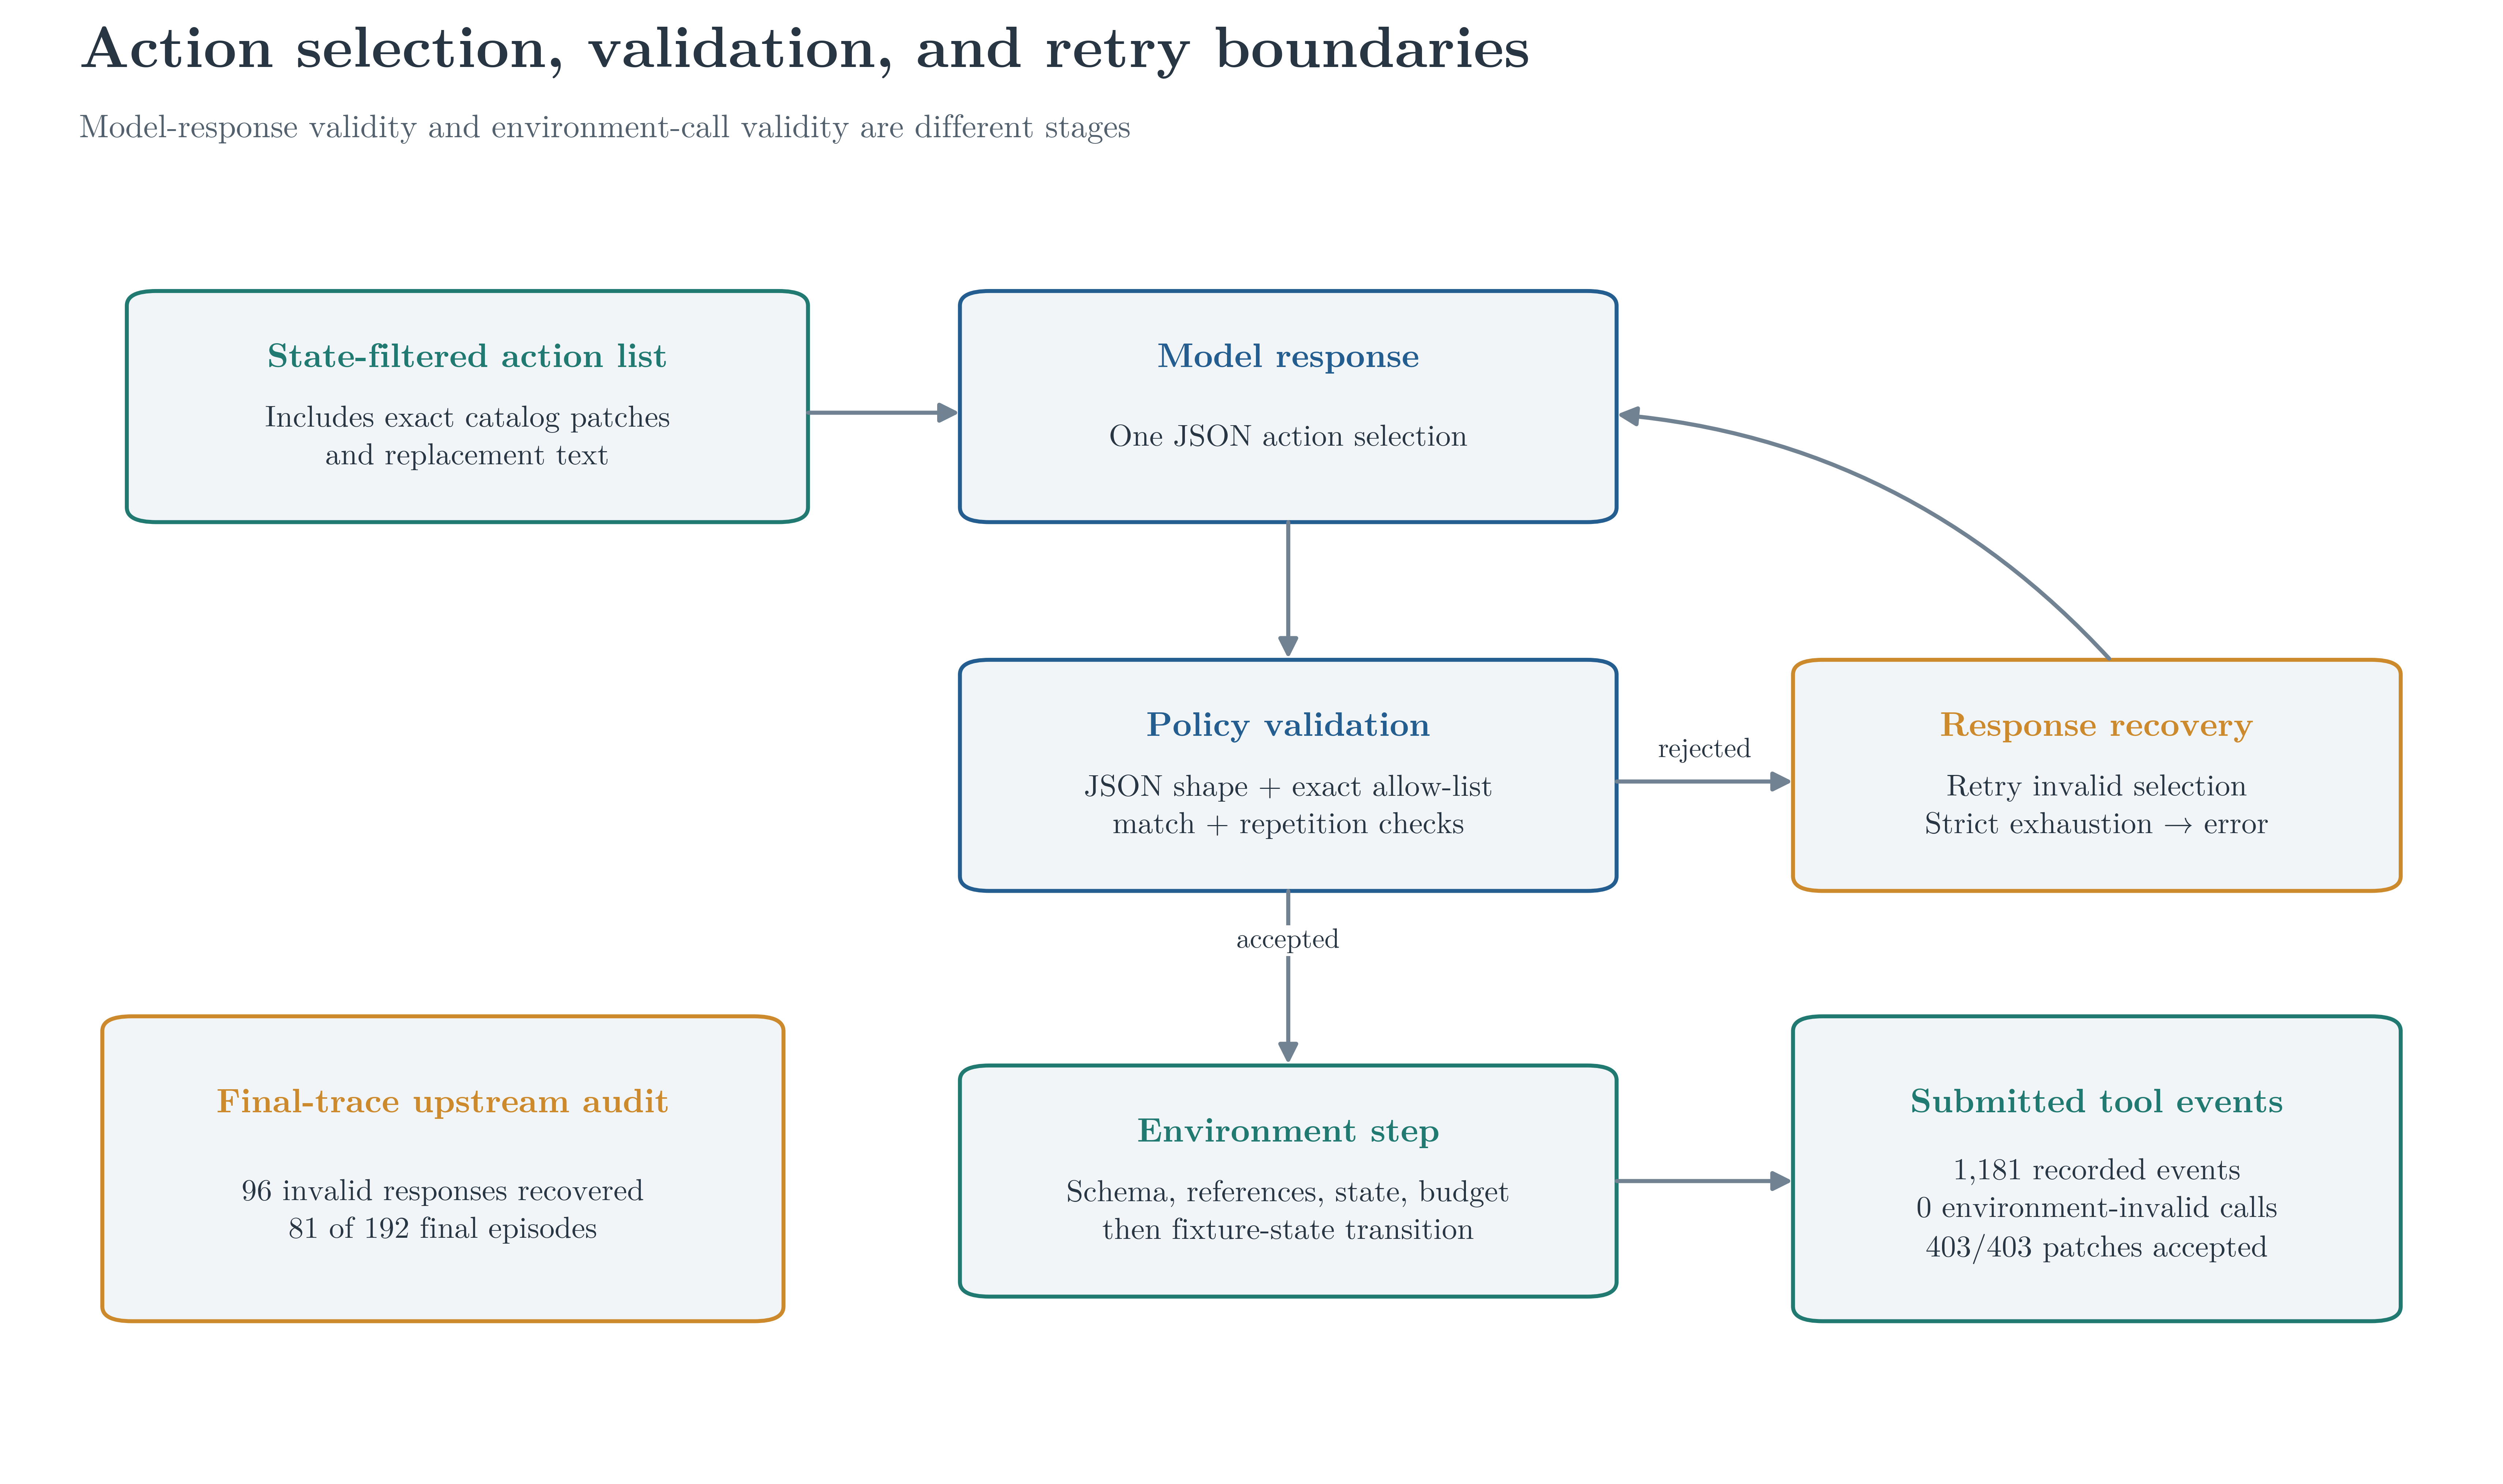
\includegraphics[width=\textwidth,height=0.68\textheight,keepaspectratio]{Images/04_action_validation.png}
\caption{Model-response validation and recovery happen before environment validation. In the final run, 96 recoverable invalid responses are distinct from zero invalid environment calls; the supplied action list exposes exact catalog patch replacements.}
\label{figure:5}
\end{figure}
\subsection{Supplied action space: a complete prompt example}
The LLM does not synthesize arbitrary patch content and submit it to a general-purpose patch tool. \texttt{list\allowbreak\_valid\allowbreak\_actions()} builds a state-dependent allow-list from the fixture: known file paths, symbols and test targets, plus exact unapplied catalog patches whose old context is still present. The complete serialized actions are embedded in every model prompt. In particular, the \texttt{apply\allowbreak\_patch} arguments contain both the catalog’s old and replacement lines. \textbf{The correct replacement text is therefore exposed to the model before it chooses an action.} The main decision is which supplied operation to select and when—not how to independently discover and generate an unrestricted code repair.

The following is a complete rendered example for the initial \texttt{math\allowbreak\_ops/sum\allowbreak\_bounds} fixture, independent agent 0, two agents, a 12-call budget, and no prior actions. It includes the entire valid-action list as the model receives it; JSON indentation is compacted for readability, without changing values or action order:

\begin{Verbatim}[breaklines=true,breakanywhere=true,fontsize=\footnotesize]
You are independent agent 0. Choose the next useful action from the shared environment state without assuming another agent will perform it.
Choose exactly one action from valid_actions. Match both tool_name and arguments exactly; do not invent tools, arguments, paths, symbols, tests, or patches.
Make task progress: do not repeat an exact recent action when another valid action is available. Do not retrieve an already observed file or search an already observed symbol. Prefer a valid apply_patch that addresses a described defect; after required patches, run relevant tests and then finalize the ticket.
Return only a JSON object with this shape:
{"arguments": "the exact arguments object from the matching valid action", "tool_name": "one tool_name from valid_actions"}

Current task and environment state:
{
  "agent_ids": [
    0,
    1
  ],
  "progress": {
    "active_regressions": [],
    "applied_patch_ids": [],
    "executed_tests": [],
    "fixed_defects": [],
    "observed_files": [],
    "observed_symbols": [],
    "progress_state": "not_started",
    "step_budget": 12,
    "step_count": 0
  },
  "recent_actions": [],
  "task": {
    "description": "The primary function subtracts instead of adds, and the helper drops the last item.",
    "title": "Fix addition and clamp behavior",
    "template_id": "math_ops",
    "variant_id": "sum_bounds"
  },
  "valid_actions": [
    {"arguments": {"path": "src/math_ops_sum_bounds.py"}, "tool_name": "retrieve_file"},
    {"arguments": {"path": "tests/test_math_ops_sum_bounds.py"}, "tool_name": "retrieve_file"},
    {"arguments": {"name": "compute_total"}, "tool_name": "search_symbol"},
    {"arguments": {"name": "window_values"}, "tool_name": "search_symbol"},
    {"arguments": {}, "tool_name": "run_tests"},
    {"arguments": {"test_target": "tests/test_math_ops_sum_bounds.py::full"}, "tool_name": "run_tests"},
    {"arguments": {"test_target": "tests/test_math_ops_sum_bounds.py::targeted"}, "tool_name": "run_tests"},
    {"arguments": {"patch": "*** Update File: src/math_ops_sum_bounds.py\n- return value - 4\n+ return value + 4"}, "tool_name": "apply_patch"},
    {"arguments": {"patch": "*** Update File: src/math_ops_sum_bounds.py\n- return items[:-1]\n+ return items[:]"}, "tool_name": "apply_patch"}
  ]
}
\end{Verbatim}
At this initial state finalization is absent from the list; it is added only after at least one patch or test action. Once a patch is applied, that patch is removed from subsequent lists, and a patch is offered only while its exact old text remains in the simulated file. This filtering prevents the policy from submitting most malformed, unknown, premature, or already-consumed operations in the first place. It is a material property of the task, not incidental prompt formatting.

Accordingly, the final-run figures of zero environment-invalid tool calls and 403/403 accepted patches (100\%) primarily show that selected calls complied with the supplied schemas, allow-list, and fixture catalog. They do \textbf{not} measure the ability to invent a correct replacement or the quality of an unrestricted patch: only the recognized patches and their replacements were available, and \texttt{run\allowbreak\_tests} checks fixture state rather than executing patched code. The reported environment-validity metric is downstream of policy parsing and action filtering. The final summaries separately record 96 recoverable invalid model responses across 81 episodes; strict handling prevented fallback actions, but those upstream response retries are not counted as environment-invalid tool calls. The two rates therefore describe different stages of this constrained pipeline.

\section{Policy adapters and turn-taking}
All policies implement the same \texttt{next\allowbreak\_action(environment)} interface and return a \texttt{PolicyAction} containing an agent ID, tool name, and arguments. \texttt{run\allowbreak\_policy\allowbreak\_episode()} repeatedly requests one action, passes it to \texttt{environment.step()}, and appends the resulting event until the environment is terminal or a policy has no action. This is sequential turn-taking against shared state. The architecture does not launch simultaneous agent calls or provide direct agent-to-agent messaging.

The scripted \texttt{single\allowbreak\_agent} policy follows a fixed sequence: retrieve the source, inspect the primary symbol, apply the primary patch, run targeted tests, apply the helper patch, run the full target, then finalize. \texttt{random\allowbreak\_policy} samples from current valid actions and randomly assigns an agent. \texttt{independent\allowbreak\_multi\allowbreak\_agent} cycles through per-agent retrieval, patch, test, or review plans, skipping candidates made invalid by shared state. \texttt{prompted\allowbreak\_coordination} follows the deterministic shared plan from \texttt{build\allowbreak\_demo\allowbreak\_actions()}, distributing inspection, patches, tests, and finalization. All remain sequential; “prompted” here names a scripted plan, not an LLM treatment.

The final experiment compares the three model-backed adapters, \texttt{llm\allowbreak\_single\allowbreak\_agent}, \texttt{llm\allowbreak\_independent\allowbreak\_multi\allowbreak\_agent}, and \texttt{llm\allowbreak\_prompted\allowbreak\_coordination}. The following table describes the implemented conditions; “agent” denotes an operational role in this sequential adapter, not necessarily an independently instantiated model or mind.

\begin{table}[htbp]
\centering
\small
\setlength{\tabcolsep}{4pt}
\begin{tabularx}{\linewidth}{|Y|Y|Y|Y|}
\hline
\textbf{Dimension} & \textbf{Single-agent} & \textbf{Independent multi-agent} & \textbf{Prompted coordination} \\
\hline
Agent count & 1 (agent 0) & 2 (agents 0 and 1) & 2 (agents 0 and 1) \\
\hline
Exact role instruction & “You are the single software agent responsible for completing the bugfix ticket within the remaining step budget.” & “You are independent agent \{agent\allowbreak\_id\}. Choose the next useful action from the shared environment state without assuming another agent will perform it.” & “You are a shared coordinator. Choose the next useful action and assign it to the agent best positioned to perform it.” \\
\hline
Actor selection & The sole action is attributed to agent 0; the model returns no agent ID. & The adapter selects the actor by turn index (\texttt{turn\allowbreak\_index \% num\allowbreak\_agents}). The model chooses a tool and arguments but cannot change the scheduled actor. & The adapter computes a preferred alternating actor, but the model is asked to return \texttt{agent\allowbreak\_id} and can assign the selected action to either current agent. \\
\hline
Information available on each decision & Current task and shared environment state, the last six selected actions (actor, tool, and arguments), agent IDs, and current valid actions. & The same shared task/environment state and last-six-action history are supplied on every turn, including actions attributed to either agent. & The same shared task/environment state and last-six-action history are supplied; the model additionally sees both agent IDs and chooses the actor attribution. \\
\hline
Private memory or independent context & None maintained between decisions beyond the shared policy-level action history. & No per-agent memory, private observation, or persistent agent-specific model context. Both nominal agents’ turns use the same policy-level history and shared environment. & No private agent memory or separate agent contexts. One coordinator decision process assigns actions to nominal agents. \\
\hline
Stopping rule & Shared rule: choose actions until finalization, budget exhaustion, or no valid action remains. & Same shared rule; actor alternation does not itself end an agent’s participation or the episode. & Same shared rule; the coordinator may select finalization from the valid actions, but the episode can also stop if no action is returned or the budget is exhausted. \\
\hline
\end{tabularx}
\caption{Policy conditions and design differences}
\end{table}
In the independent instruction, \texttt{\{agent\allowbreak\_id\}} is rendered as the scheduled actor ID (0 or 1) for that turn.

All three LLM conditions use the same model configuration and common action-selection instructions, appended verbatim after the role instruction:

\begin{quote}
Choose exactly one action from valid\allowbreak\_actions. Match both tool\allowbreak\_name and arguments exactly; do not invent tools, arguments, paths, symbols, tests, or patches. Make task progress: do not repeat an exact recent action when another valid action is available. Do not retrieve an already observed file or search an already observed symbol. Prefer a valid apply\allowbreak\_patch that addresses a described defect; after required patches, run relevant tests and then finalize the ticket.
\end{quote}

Each request asks for JSON containing \texttt{tool\allowbreak\_name} and \texttt{arguments}; only the coordinator prompt also requires \texttt{agent\allowbreak\_id}. The environment exposes finalization only after an update or test action and independently enforces the shared step budget. Thus a nominal agent is distinguished operationally by its role instruction and/or turn/assignment rule plus the \texttt{agent\allowbreak\_id} attached to its action. There is no persistent, autonomous per-agent decision state: each action is selected in a new model request using shared state, while the coordinator condition uses one decision process to choose both the action and its actor attribution. These conditions should not be described as two independent model instances collaborating.

\textbf{Design implication for interpretation.} Prompted coordination changes two factors together: it replaces the independent-agent role instruction with a coordinator instruction, and it gives the model control over actor assignment rather than fixing the actor by alternation. Therefore, the independent-versus-prompted comparison cannot isolate a prompt effect. Differences in completion, action use, participation, or stopping may arise from the instruction, assignment freedom, or their interaction. The observed agent-level workload differences are especially sensitive to this bundled assignment mechanism. The condition contrast is descriptive of two implemented policies, not a causal estimate of coordination prompting. Isolating a prompt effect would require holding actor selection constant across prompt conditions (or a factorial design crossing instruction with fixed-versus-model-selected assignment); the current dataset does not contain those controls.

\begin{figure}[htbp]
\centering
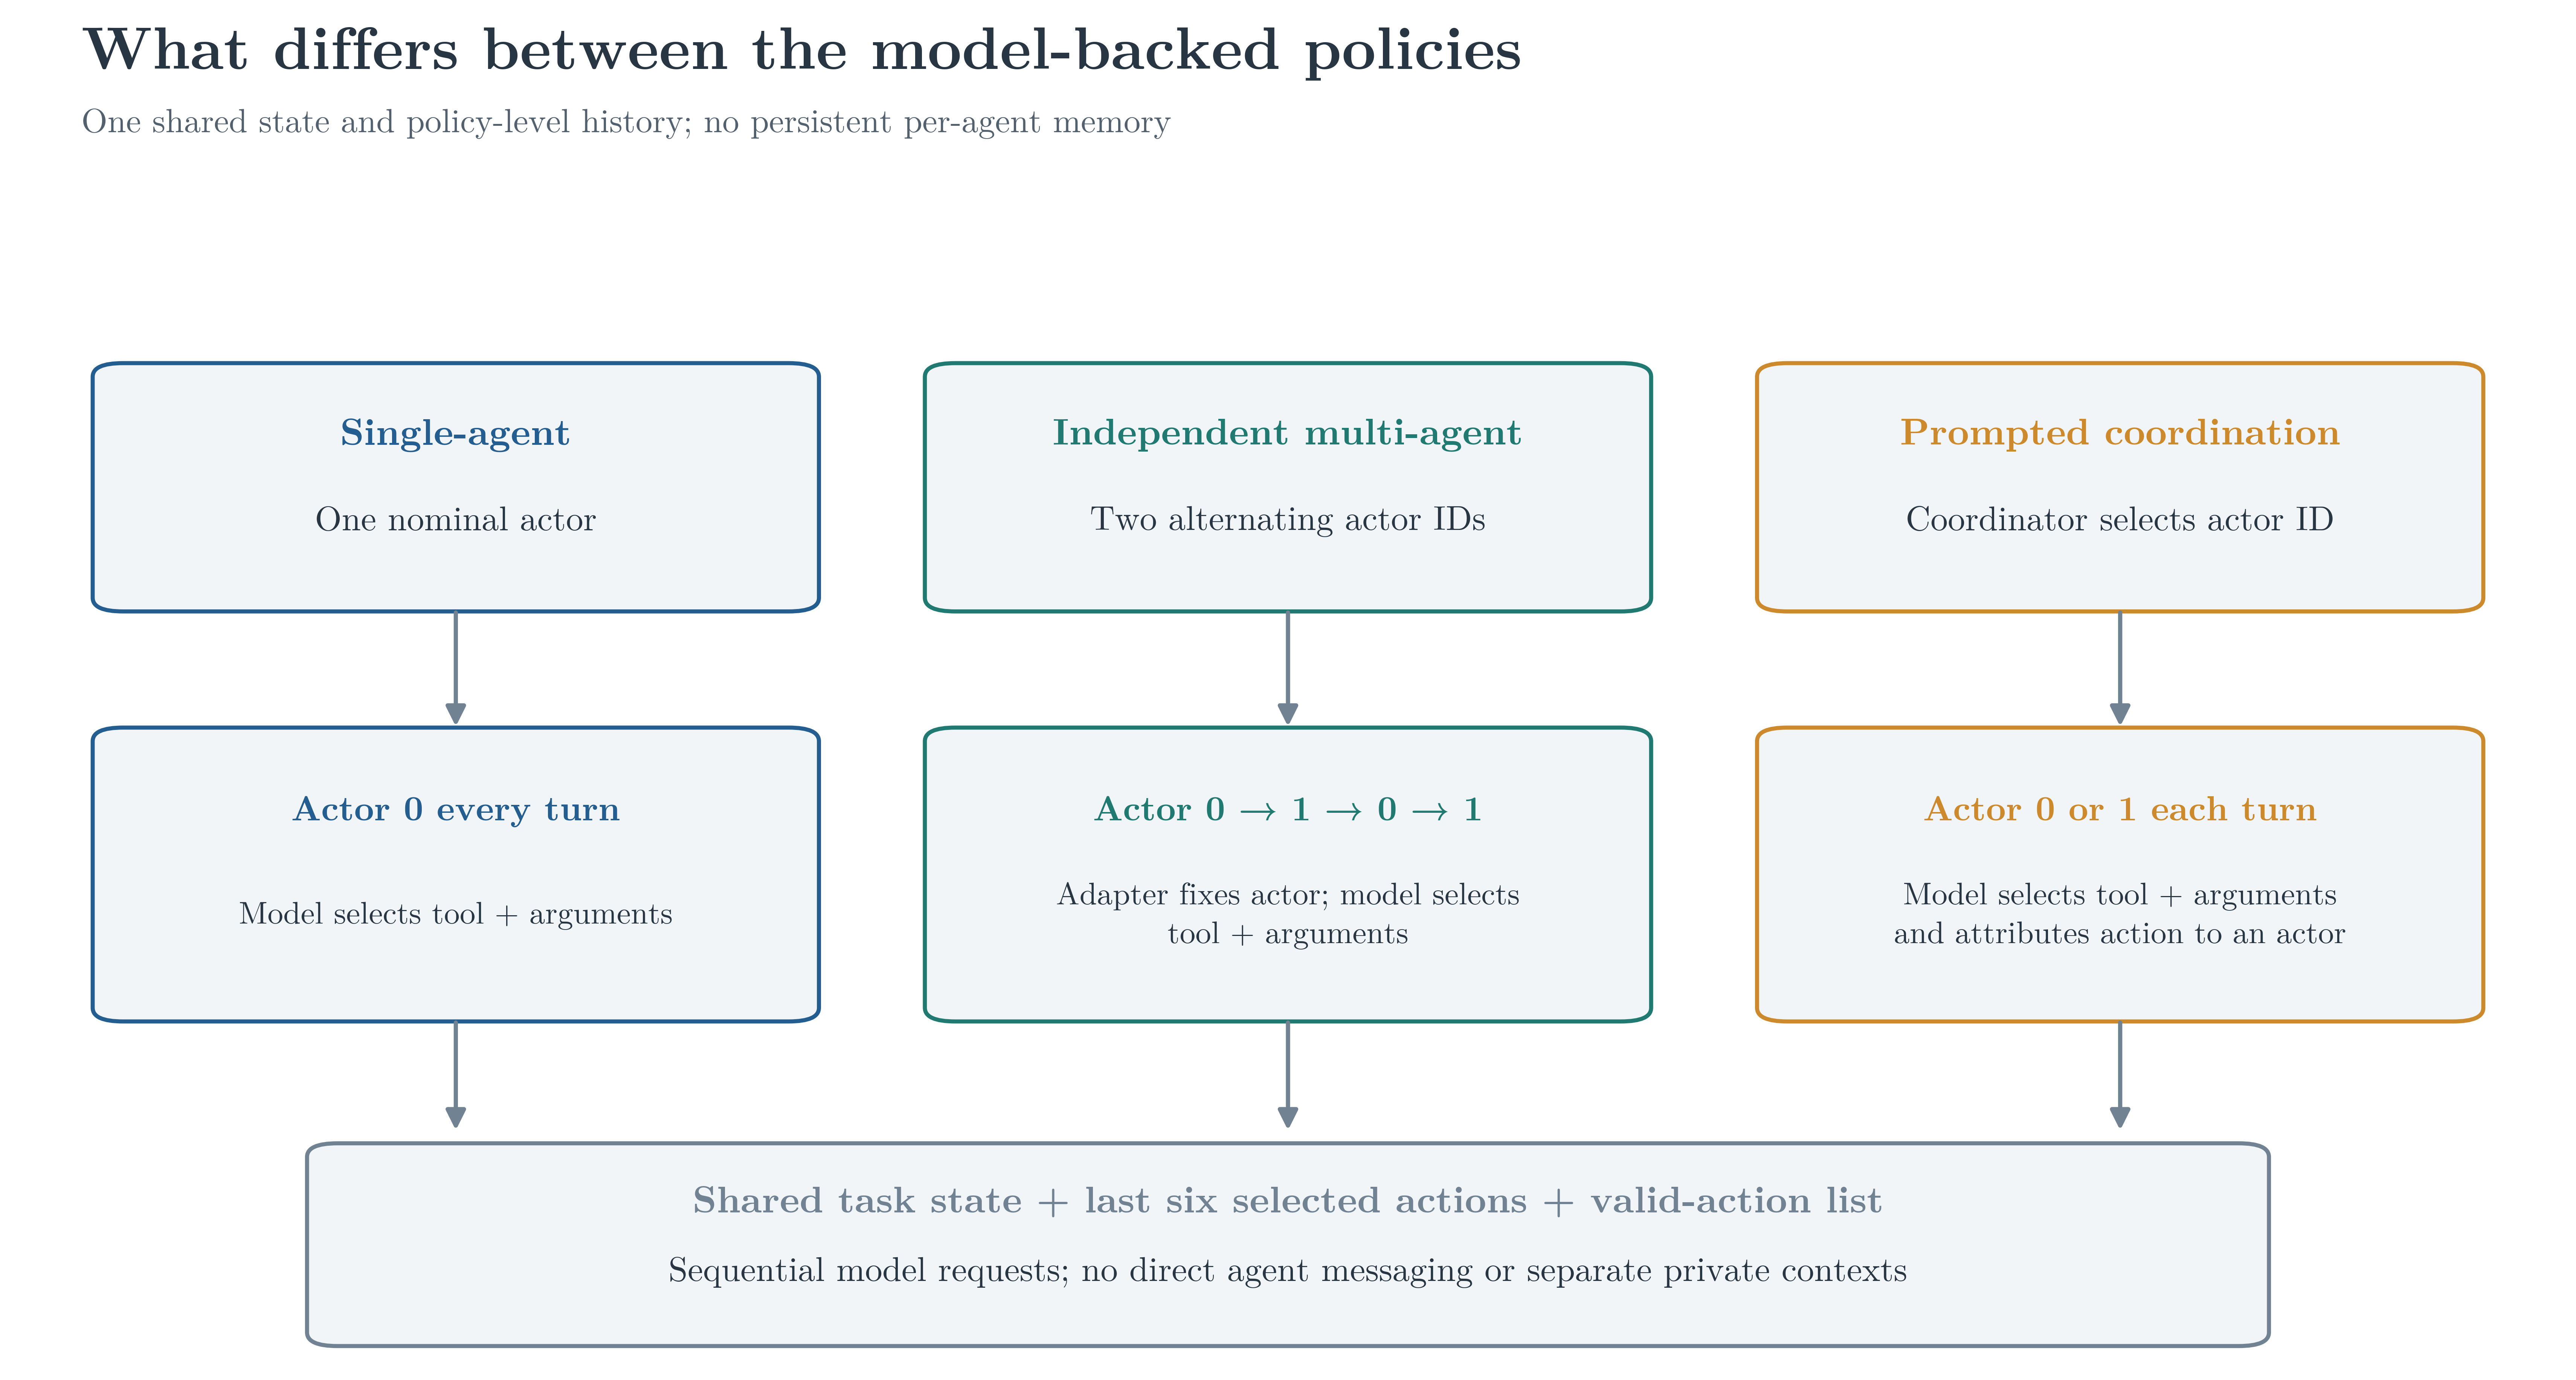
\includegraphics[width=\textwidth,height=0.68\textheight,keepaspectratio]{Images/06_policy_assignment.png}
\caption{Single-agent actions use actor 0; the independent adapter alternates actor IDs; prompted coordination lets one action-selection process assign an actor. Assignment authority and role wording vary together.}
\label{figure:6}
\end{figure}
\section{LLM client, action parsing, and audit}
The LLM client reads settings with environment-variable overrides. It resolves \texttt{openai/} and \texttt{azureai/} prefixes and recognizes slash-qualified OpenRouter names, although its client builder supports OpenAI and Azure AI only. Azure requests use the configured API version and normalized endpoint. The thesis configuration uses \texttt{azureai/gpt-5-mini}; credentials remain in environment variables. Synchronous requests use JSON-object mode and choose \texttt{max\allowbreak\_completion\allowbreak\_tokens} for GPT-5/reasoning prefixes, otherwise \texttt{max\allowbreak\_tokens}.

The policy prompt includes task identity and description, current progress, the last six actions in the shared policy-level action history, all agent IDs, and the current valid-action list. It appends common instructions to select exactly one allowed action, avoid repeating an unproductive action, prefer a valid defect-fixing patch, and run relevant tests before finalizing. The single-agent and independent adapters request a JSON object with \texttt{tool\allowbreak\_name} and \texttt{arguments}; the independent adapter’s actor is imposed by alternation. Coordinator mode additionally requests \texttt{agent\allowbreak\_id}, making the model responsible for actor assignment. This is an additional procedural difference, not just a different wording of the same prompt. The policy parses a dictionary directly or extracts and JSON-decodes response content. It then requires a string tool name and object arguments, validates any returned agent ID, and matches the tool-plus-arguments exactly against one currently valid action. Thus the client requests JSON syntax, while the policy and environment enforce the action contract; a syntactically valid but invented action is still rejected. The two nominal independent agents have no separate prompt histories or private memory: every call receives shared environment state and the same policy-level action history, with only the role text and scheduled ID varying by turn. The coordinator, in contrast, is a single action-selection process with authority to label either nominal agent as actor.

Consequently, the final run’s independent-versus-prompted contrast is a comparison of bundled policies, not a prompt-only intervention. Prompt wording and actor-selection authority vary together while other features—model configuration, environment, available tools, and common instructions—are shared. No statistical adjustment to these observations can recover a prompt-only effect absent a condition that holds assignment behavior constant; causal attribution requires a redesigned matched or factorial experiment.

There are two retry layers. Within \texttt{chat\allowbreak\_json()}, the client retries retryable connection, timeout, rate-limit, and server errors up to the configured maximum (five by default), with exponential delay and jitter. Authentication, quota, access, and other non-retryable failures are classified and returned as request errors when soft fallback is disabled. At the policy layer, malformed JSON, wrong response shapes, non-matching actions, and unproductive repeats can prompt another action-selection attempt; the default is two parse attempts. The retry prompt includes the prior validation error and again requests one exact valid action. The policy audit records invalid responses, model errors, fallback responses and reasons, and locally selected fallback actions.

With non-strict mode, a client initialization/request failure can produce a marked \texttt{FallbackResponse}. The policy records it and selects a valid local fallback action, preferring a non-repeated update or another available action; this action is not an unmodified model choice. If parse attempts are exhausted, the adapter also falls back locally. In strict mode, a marked client fallback raises \texttt{LLMFallbackError}; a model-call error raises \texttt{LLMCallError}; and a response that remains invalid raises \texttt{LLMResponseError}. The thesis runner enables strict mode and stores the policy audit. Completed-artifact validation rejects a summary marked strict if it records either a fallback response or fallback action. Runner classification treats strict fallback, exhausted client/API failures, authentication/access/quota errors, and artifact/configuration failures as non-retryable collection failures; a final invalid model response is classified as an isolated retryable episode failure. This audit makes recovery visible rather than equating every environment action with an accepted model response. Client-format, retry metadata, policy retry/fallback, and strict rejection behavior are exercised in test\allowbreak\_llm\allowbreak\_client.py, test\allowbreak\_tool\allowbreak\_use\allowbreak\_baselines.py, and test\allowbreak\_run\allowbreak\_baseline\allowbreak\_sweep.py.

\section{Manifest, assignment, progress, and resumability}
Before a sweep, the runner builds a manifest with one item per baseline, fixture, and repetition. A manifest ID encodes baseline, repetition, seed, template, and variant. For the thesis configuration, the deterministic builder traverses all 16 fixtures and four repetitions, assigning each fixture/repetition a seed beginning at 200, then adds each of three conditions. That yields 64 manifest items per condition and 192 total. Each policy comparison therefore uses the same named fixture, repetition, and seed identity. In seed-list pilot mode, a seeded selection maps each seed to a fixture; in the thesis fixture-repetition mode, the fixture is explicit in each manifest item and the environment receives that fixture directly.

The frozen \texttt{manifest.json} and \texttt{experiment\allowbreak\_config.json} preserve planned identities and settings. On resume, the runner rebuilds the plan and refuses to continue if the manifest differs or if comparable frozen configuration fields differ (apart from creation time). \texttt{progress.json} records each manifest item as \texttt{completed} or \texttt{failed}, along with batch checkpoints and derived completed, failed, pending, and run-complete fields. Completed IDs are skipped on resume after their artifacts have been rediscovered and checked. Failed IDs can be selected with the explicit retry mode; a separate option permits a run to continue after an isolated retryable response failure, while fatal failures abort the batch. \texttt{aggregate\allowbreak\_summary.json} is recomputed from completed manifest records, with failed and pending items reported separately. An error/retry record is a collection-attempt record, not an additional completed episode.

Before accepting output or resuming, \texttt{\allowbreak\_validate\allowbreak\_completed\allowbreak\_artifact()} checks required files, summary versions/outcome/identity, replay-spec agreement, a matching JSONL header, event record types/count, fixture identity, and strict fallback counts. Progress and error records are checked against manifest identity and status. These are structural checks, not checksums. The targeted audit reported in Section 9.6 later checked identity, counts, event ordering, and hash consistency; comprehensive schema, semantic, and replay validation remain incomplete. Replay metadata does not make model output deterministic. Manifest balance, explicit fixture replay, resume without duplicates, retry status, and strict fallback are tested in test\allowbreak\_run\allowbreak\_baseline\allowbreak\_sweep.py.

\begin{figure}[htbp]
\centering
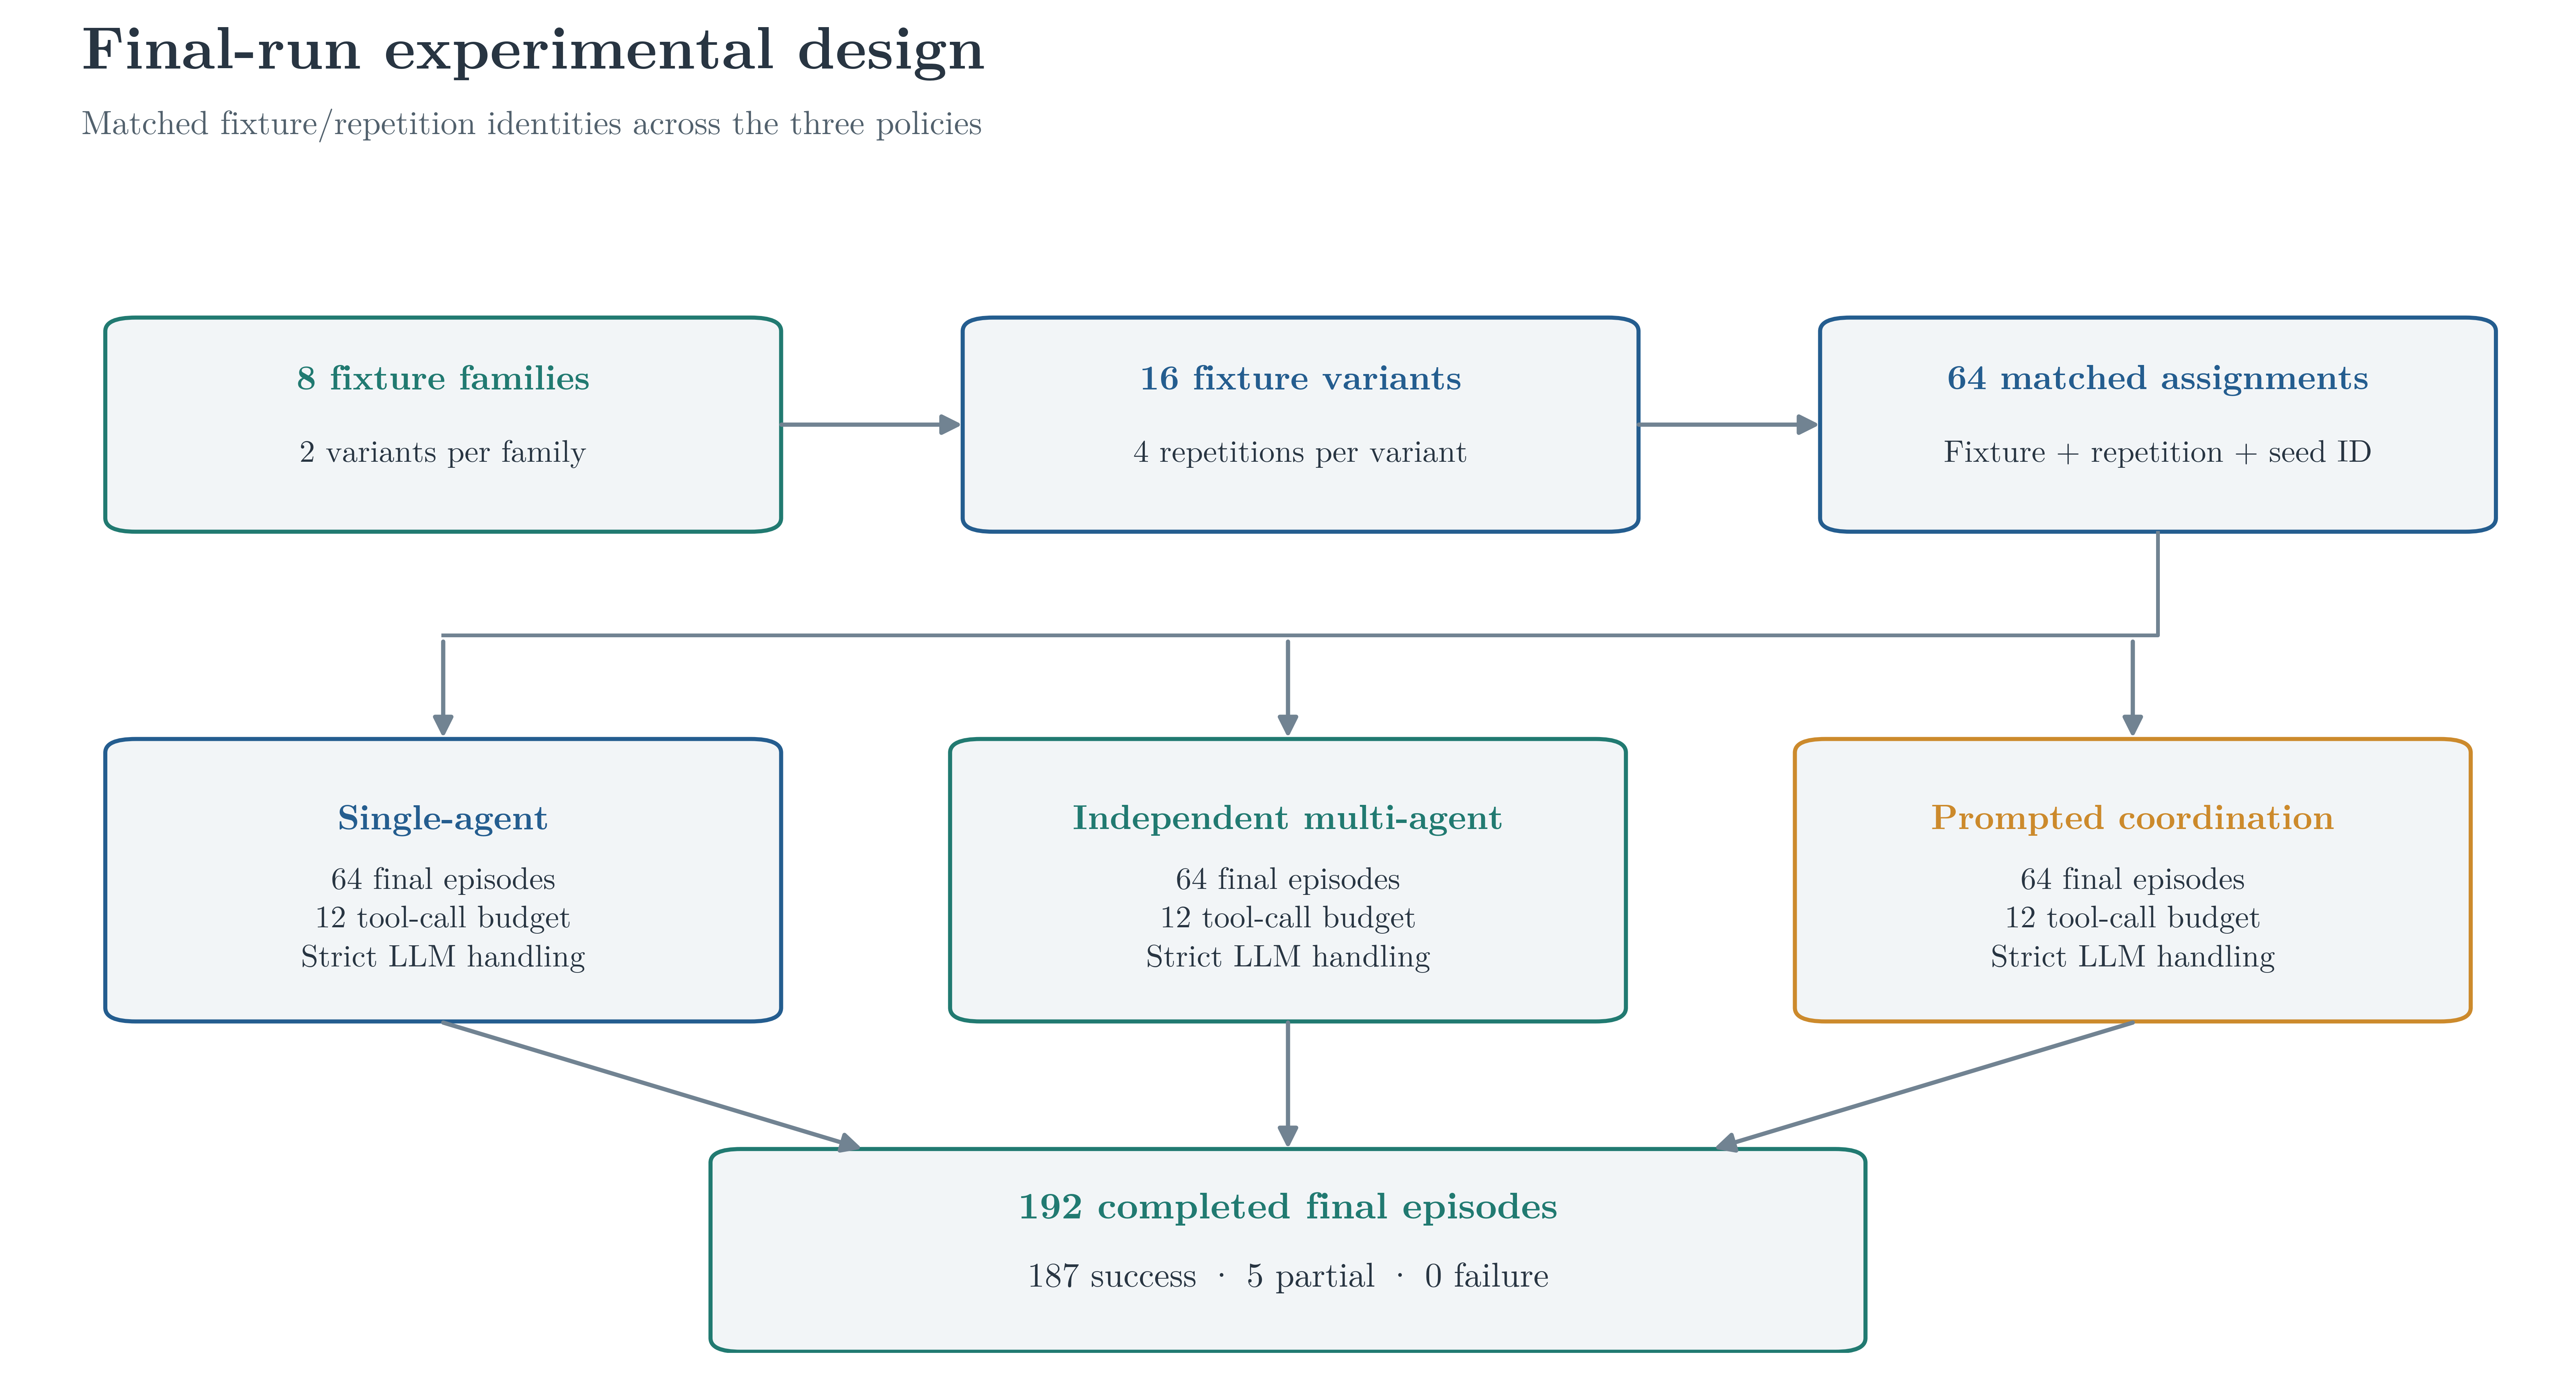
\includegraphics[width=\textwidth,height=0.68\textheight,keepaspectratio]{Images/05_matched_design.png}
\caption{The final Phase 2 run pairs all three conditions over the same 16 fixture variants and four repetitions, giving 64 episodes per condition and 192 total.}
\label{figure:7}
\end{figure}
\section{Canonical artifacts, action abstractions, and export}
Each episode is persisted by \texttt{persist\allowbreak\_episode\allowbreak\_run()} as three canonical files: \texttt{episode.jsonl}, \texttt{summary.json}, and \texttt{task\allowbreak\_fixture.json}. The JSONL starts with an \texttt{episode\allowbreak\_header} containing schema/environment versions, config hash, seed, fixture, agent count, step budget, and timestamp. Each subsequent \texttt{tool\allowbreak\_event} has a sequence ID, actor, tool and arguments, validity and invalid reason, abstraction, progress state and outcome, output, current fixed defects/regressions/patch IDs, step count, and timestamp. The summary holds episode-level outcome, progress, step counts, invalid-call counts/rate, test results, patch IDs, and replay specification; the runner enriches it with policy/model identity, condition-level measures, and LLM audit. The fixture JSON preserves the task specification used to interpret the trace.

The action abstraction maps successful retrieval/search calls to \texttt{retrieve}, test calls to \texttt{verify}, patches to \texttt{update}, and finalization to \texttt{finalize}. Invalid calls receive \texttt{error\allowbreak\_or\allowbreak\_noop}. \texttt{validate\allowbreak\_abstraction\allowbreak\_invariants()} checks that events use one of these categories before the episode returns. These mutually exclusive categories bridge tool names and a compact trajectory representation; they do not purport to label intention or semantic contribution.

\texttt{export\allowbreak\_trajectory\allowbreak\_data.py} reads episode headers, events, and optional summaries into event-level and episode-level tables. Event rows retain condition-independent identity, event order, tool, validity, reason, abstraction, state, outcome, arguments/output, and defect/patch state. Summary rows preserve outcome, counts, tests, invalid-call counters, patch information, and replay specification. CSV is written when rows exist; Parquet is optional and depends on the installed pandas/parquet stack. \texttt{export\allowbreak\_manifest.json} records episode/event row counts, output paths, optional Parquet status, and parse issues. These exports are derived artifacts; the per-episode JSONL and summary remain the canonical records.

\section{Coordination analysis and visualization}
The episode analysis in coordination\allowbreak\_analysis.py derives three representations for each agent: the full ordered abstraction trace; a five-element count vector for retrieval, verification, update, finalization, and error/no-op, with each count capped at two; and a six-category \texttt{coarsened\allowbreak\_action\allowbreak\_profile}. The profile applies priority in this order: any error/no-op, finalized, updated, verified, retrieved, then no actions. Consequently it deliberately discards action order and many count distinctions to reduce categorical state cardinality. The analysis report compares representations but defaults to \texttt{coarsened\allowbreak\_action\allowbreak\_profile}.

\textbf{Worked example of the profile rule.} Counts are ordered as \texttt{(retrieve, verify, update, finalize, error/no-op)} and capped at two. Compare two possible per-agent traces from separate episodes: an agent retrieves a file, patches it, runs tests, and finalizes, yielding \texttt{(1,1,1,1,0)}; another agent only finalizes, yielding \texttt{(0,0,0,1,0)}. Both map to \texttt{finalized}. The priority rule therefore erases the first trace's retrieve/verify/update history and cannot distinguish it from the finalize-only trace. In the episode-level joint profile, the location of \texttt{finalized} identifies which actor ID was assigned the terminal event; the other profile retains only that agent's highest-priority non-finalization category. This encoding is compact, but it directly entangles the source variable with stopping behavior.

The analysis reports exploratory plug-in categorical mutual information in bits between the joint two-agent profile \$(A\allowbreak\_0,A\allowbreak\_1)\$ and outcome \$Y\$ (\texttt{success}, \texttt{partial}, or \texttt{failure}): \$I((A\allowbreak\_0,A\allowbreak\_1);Y)=\textbackslash\{\}sum\allowbreak\_\{a\allowbreak\_0,a\allowbreak\_1,y\}p(a\allowbreak\_0,a\allowbreak\_1,y)\textbackslash\{\}log\allowbreak\_2\textbackslash\{\}frac\{p(a\allowbreak\_0,a\allowbreak\_1,y)\}\{p(a\allowbreak\_0,a\allowbreak\_1)p(y)\}\$. It quantifies empirical dependence between these encoded categories and outcome in the eligible episodes. It is not an established coordination measure, temporal measure, causal effect, measure of success rate, or the paper's time-delayed mutual information / PID synergy. Because the profile prioritizes finalization and discards event order and counts, its MI may primarily reflect who is attributed the stopping action and which coarse category remains for the other actor. Joint profiles can be associated with outcomes even when agents act independently, and meaningful cross-agent division of work can disappear under this compression. The estimate is therefore exploratory unless the action profile is shown to validly represent coordination and its relationship to coordination is independently established; behavioral trace analysis, richer encodings, and controlled coordination ablations would be needed for that interpretation. The saved report includes smoothing sensitivity, bootstrap intervals, and outcome-label permutation diagnostics, but these do not repair the construct-validity or design limitations. Sanity tests cover estimator behavior (test\allowbreak\_coordination\allowbreak\_metrics.py); representation and eligibility are tested in test\allowbreak\_coordination\allowbreak\_analysis.py.

The estimator requires two observed agent traces, so single-agent episodes are excluded from the two-agent MI dataset. The separate one-agent reference report computes a one-source association and explicitly labels it as a reference, not a two-agent coordination estimate. This is a structural limitation, not a missing-data workaround. Small samples, many distinct joint categories, and constant or nearly constant outcomes constrain interpretation: high-cardinality states can yield sparse frequency tables and unstable plug-in estimates, while a constant outcome contains no empirical outcome variation for MI to explain. The scripted pilot's saved report demonstrates why coarsening was introduced: full traces separated many episodes into distinct categories, while the profile merged some patterns; the final thesis run likewise has only a few observed joint profiles and two observed outcome classes in each multi-agent condition. Those reductions improve tractability but do not eliminate estimator or design limitations. A constant all-success single-agent arm cannot serve as evidence of two-agent coordination, and the final report properly leaves its pairwise estimate absent.

Finally, \texttt{results\allowbreak\_visualization.py} generates PDFs of eligible MI with bootstrap intervals, invalid-call rate, mean calls, patch acceptance versus recovery, and a second panel of MI, test-call proportion, and permutation p-values. These plots add no inference beyond the saved statistics. \texttt{validation.md} records remaining needs: full-data abstraction audits, human labeling, correlations, and deterministic scripted replay. Pipeline execution therefore supports traceability, not construct validity by itself.

\begin{figure}[htbp]
\centering
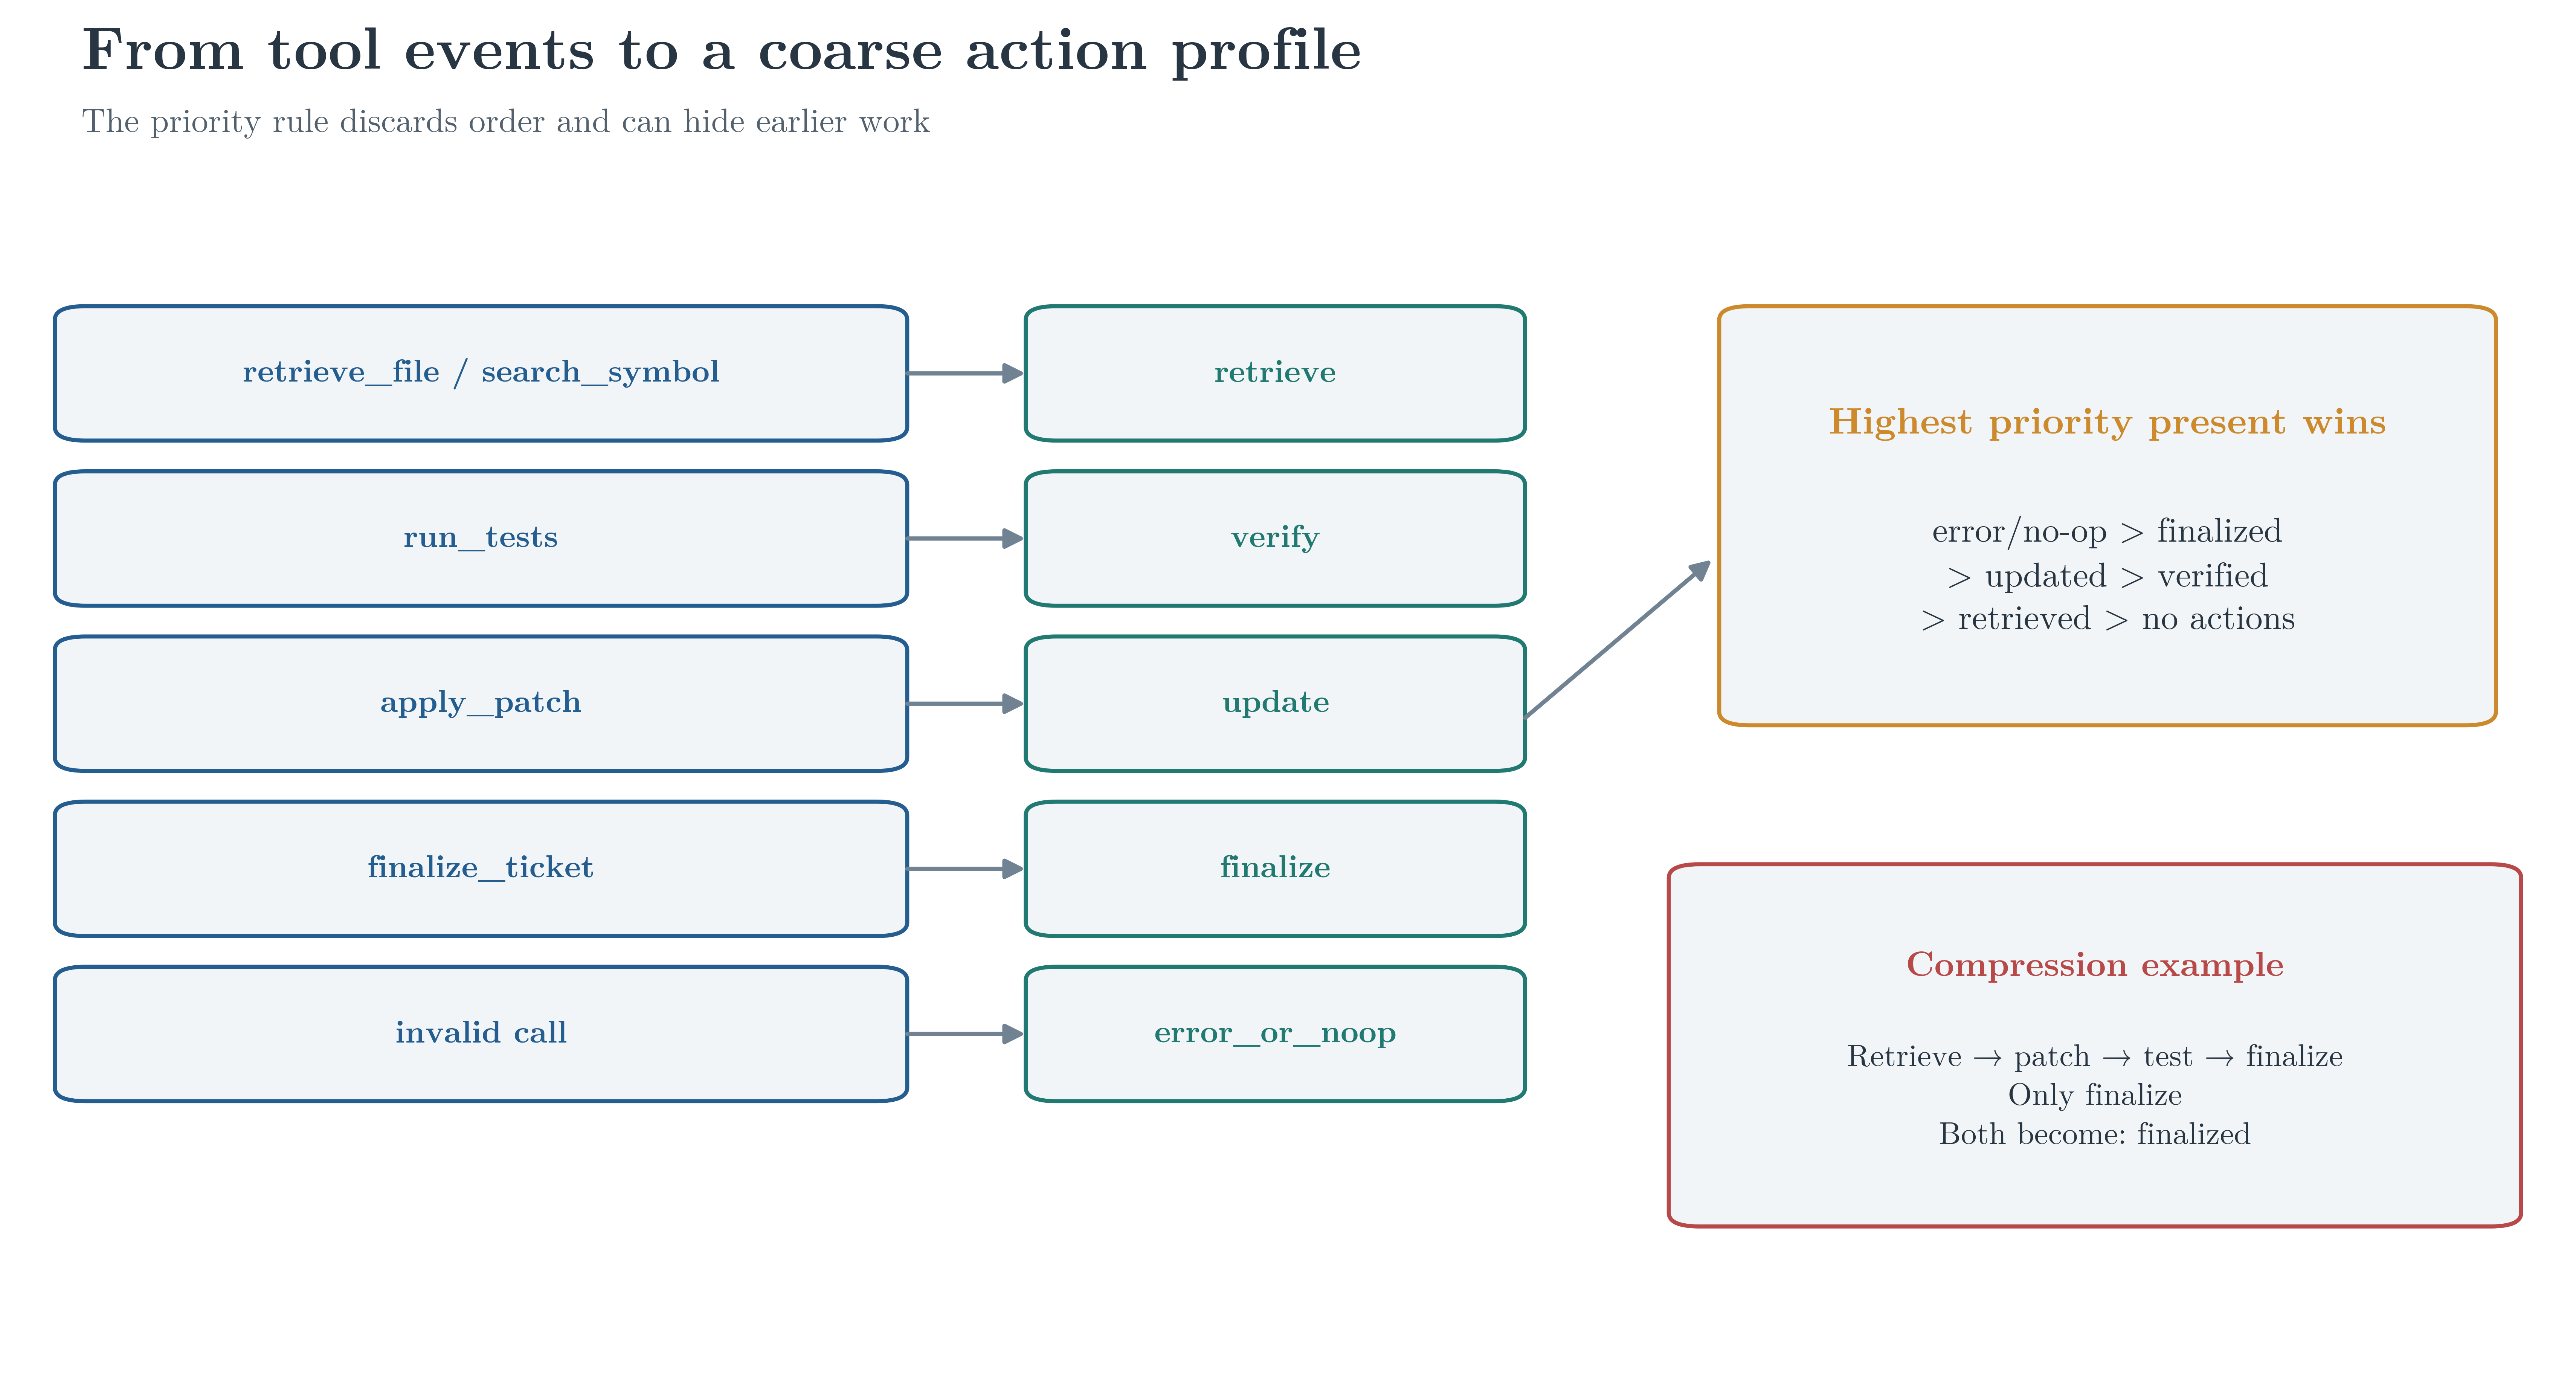
\includegraphics[width=\textwidth,height=0.68\textheight,keepaspectratio]{Images/07_action_abstraction.png}
\caption{Phase 2 tools are mapped to coarse action categories for analysis. This representation supports trace summaries but loses ordering and within-category detail.}
\label{figure:8}
\end{figure}
\chapter{Experimental Progression}
\label{chapter-06}
\thispagestyle{plain}
Phase 1 was the starting point: a repeated guessing game where each agent contributed a number from its own private history and the group received one shared directional signal. This was a simple, interpretable setting in which individual actions could be observed in relation to a collective result. Over time, persona prompts and more detailed recovery and output recording were added to the implementation. These refinements made the runs easier to inspect, although the available Phase 1 records remain a small, selected sample rather than a complete reproduction of the motivating paper.

Phase 2 was motivated by the limits of a single aggregate guess and a single feedback signal. A deterministic synthetic bug-fix task was built in which an action can retrieve information, update fixture state, verify progress, or finalize. Scripted policies allowed the environment to be checked without model-generated decisions; small model-backed pilots then exercised the action interface before the final balanced run was collected. The pilot, calibration, and final-run results in Chapters 7–9 are stages in the development and use of this Phase 2 framework, not one pooled dataset.

After the Phase 2 experiments were complete, the Phase 1 task was revisited and the \texttt{submit\allowbreak\_guess(value)} bridge was added. This later engineering check shows how a Phase 1 contribution can be represented and audited using an explicit action event while keeping the guessing rules intact. It provides a connection between the two experimental designs, not evidence that they are the same experiment or that the bridge was part of the original Phase 2 runs.

\chapter{Phase 2: Scripted Pilot}
\label{chapter-07}
\thispagestyle{plain}
\section{Purpose and scope}
A scripted pilot was first used to test whether the new environment and analysis pipeline worked end to end. It is not the final thesis dataset. Its configuration specifies the synthetic bug-fix environment, four scripted conditions, 20 episode seeds (200–219) per condition, an eight-call budget, and 80 planned episodes (\texttt{experiment\allowbreak\_config.json}). Although the configuration records \texttt{azureai/gpt-5-mini} as \texttt{model\allowbreak\_name}, none of these four policies is LLM-backed; their actions came from scripted procedures.

The unit of observation is an episode over a synthetic fixture. The configured seeds are reused across the four conditions, allowing descriptive comparisons on corresponding fixture assignments, but the policies are deterministic or pseudo-random scripted procedures rather than controlled prompt treatments. Their calls occur sequentially against a shared mutable environment. This is consequently not a test of the paper’s private-guess/shared-feedback game, and it cannot establish a paper-style emergence or synergy result.

\section{Episode reconciliation}
The run’s \texttt{progress.json} records four completed batches of 20 episodes. The 80 episode-level summaries were counted independently, and their outcomes and metrics were compared with the saved aggregate. The aggregate agrees with the episode summaries: each condition has 20 episodes; the single-agent, independent-multi-agent, and prompted-coordination conditions each have 16 successes, 4 partials, and no failures; random policy has 6 successes, 10 partials, and 4 failures. Thus there are 54 successes (67.5\%), 22 partials (27.5\%), and 4 failures (5\%) overall. These totals describe this run only.

The \texttt{exports/export\allowbreak\_manifest.json} reports 80 exported summaries, 546 events, and no collection issues. Independently summing \texttt{event\allowbreak\_count} across the 80 episode summaries also gives 546. This resolves a stale documentation discrepancy: \texttt{baseline/validation.md} reports 558 events, but neither the export manifest nor the episode artifacts support that number. The manifest also records successful CSV and Parquet writes. This confirms the existence and stated row counts of the exported artifacts, not a complete independent semantic or schema audit of every exported field.

\section{Outcomes and episode-level measures}
\begin{table}[htbp]
\centering
\fontsize{8.5}{9.5}\selectfont
\setlength{\tabcolsep}{1.5pt}
\renewcommand{\arraystretch}{1.15}
\begin{tabular}{|>{\raggedright\arraybackslash}p{2.3cm}|>{\centering\arraybackslash}p{1.4cm}|>{\centering\arraybackslash}p{1.25cm}|>{\centering\arraybackslash}p{1.25cm}|>{\centering\arraybackslash}p{1.15cm}|>{\centering\arraybackslash}p{1.7cm}|>{\centering\arraybackslash}p{1.8cm}|>{\centering\arraybackslash}p{1.7cm}|>{\centering\arraybackslash}p{1.8cm}|}
\hline
\shortstack[l]{\textbf{Scripted}\\\textbf{condition}} & \textbf{Episodes} & \textbf{Success} & \textbf{Partial} & \textbf{Failure} & \shortstack[c]{\textbf{Mean}\\\textbf{invalid-}\\\textbf{call rate}} & \shortstack[c]{\textbf{Mean}\\\textbf{calls to}\\\textbf{completion}} & \shortstack[c]{\textbf{Mean}\\\textbf{patch}\\\textbf{acceptance}} & \shortstack[c]{\textbf{Mean test}\\\textbf{call}\\\textbf{proportion}} \\
\hline
\shortstack[l]{Single agent} & 20 & 16 (80\%) & 4 (20\%) & 0 (0\%) & 0\% & 7.0 & 100\% & 28.57\% \\
\hline
\shortstack[l]{Random policy} & 20 & 6 (30\%) & 10 (50\%) & 4 (20\%) & 0\% & 6.3 & 80\% & 29.73\% \\
\hline
\shortstack[l]{Independent\\multi-agent} & 20 & 16 (80\%) & 4 (20\%) & 0 (0\%) & 0\% & 7.0 & 100\% & 28.57\% \\
\hline
\shortstack[l]{Prompted\\coordination} & 20 & 16 (80\%) & 4 (20\%) & 0 (0\%) & 0\% & 7.0 & 100\% & 28.57\% \\
\hline
\end{tabular}
\caption{Scripted pilot outcomes and operational measures}
\end{table}
The rates and means above match the aggregate and episode summaries. In the implementation, calls to completion count recorded tool events; mean invalid-call rate is invalid environment calls divided by episode steps; patch acceptance is computed per episode as valid patch calls divided by patch attempts (zero when there were no attempts); and test-call proportion is the per-episode fraction of calls that invoked \texttt{run\allowbreak\_tests} (\texttt{tool\allowbreak\_use\allowbreak\_baselines.py}, \texttt{tool\allowbreak\_use\allowbreak\_environment.py}). The aggregate reports averages of the per-episode ratios, not necessarily a ratio formed by pooling every event. The pilot recorded no invalid environment calls in any condition. This says the policies’ submitted actions passed the environment’s validity checks; it does not mean every valid action advanced the task or that all policies solved the fixture.

This test-call proportion is a narrow action-mix statistic, not an efficiency measure. The environment evaluates declared fixture defects and regression guards; it does not execute pytest or test patched repository code (\texttt{tool\allowbreak\_use\allowbreak\_environment.py}). A test call is therefore a synthetic verification operation. The reported 28.57\% for the three seven-call scripted patterns means two of seven calls were test operations. Random policy’s 29.73\% is the average of its episode-level ratios, with a variable number of actions and tests; it should not be read as a quality score for software testing.

\begin{figure}[htbp]
\centering
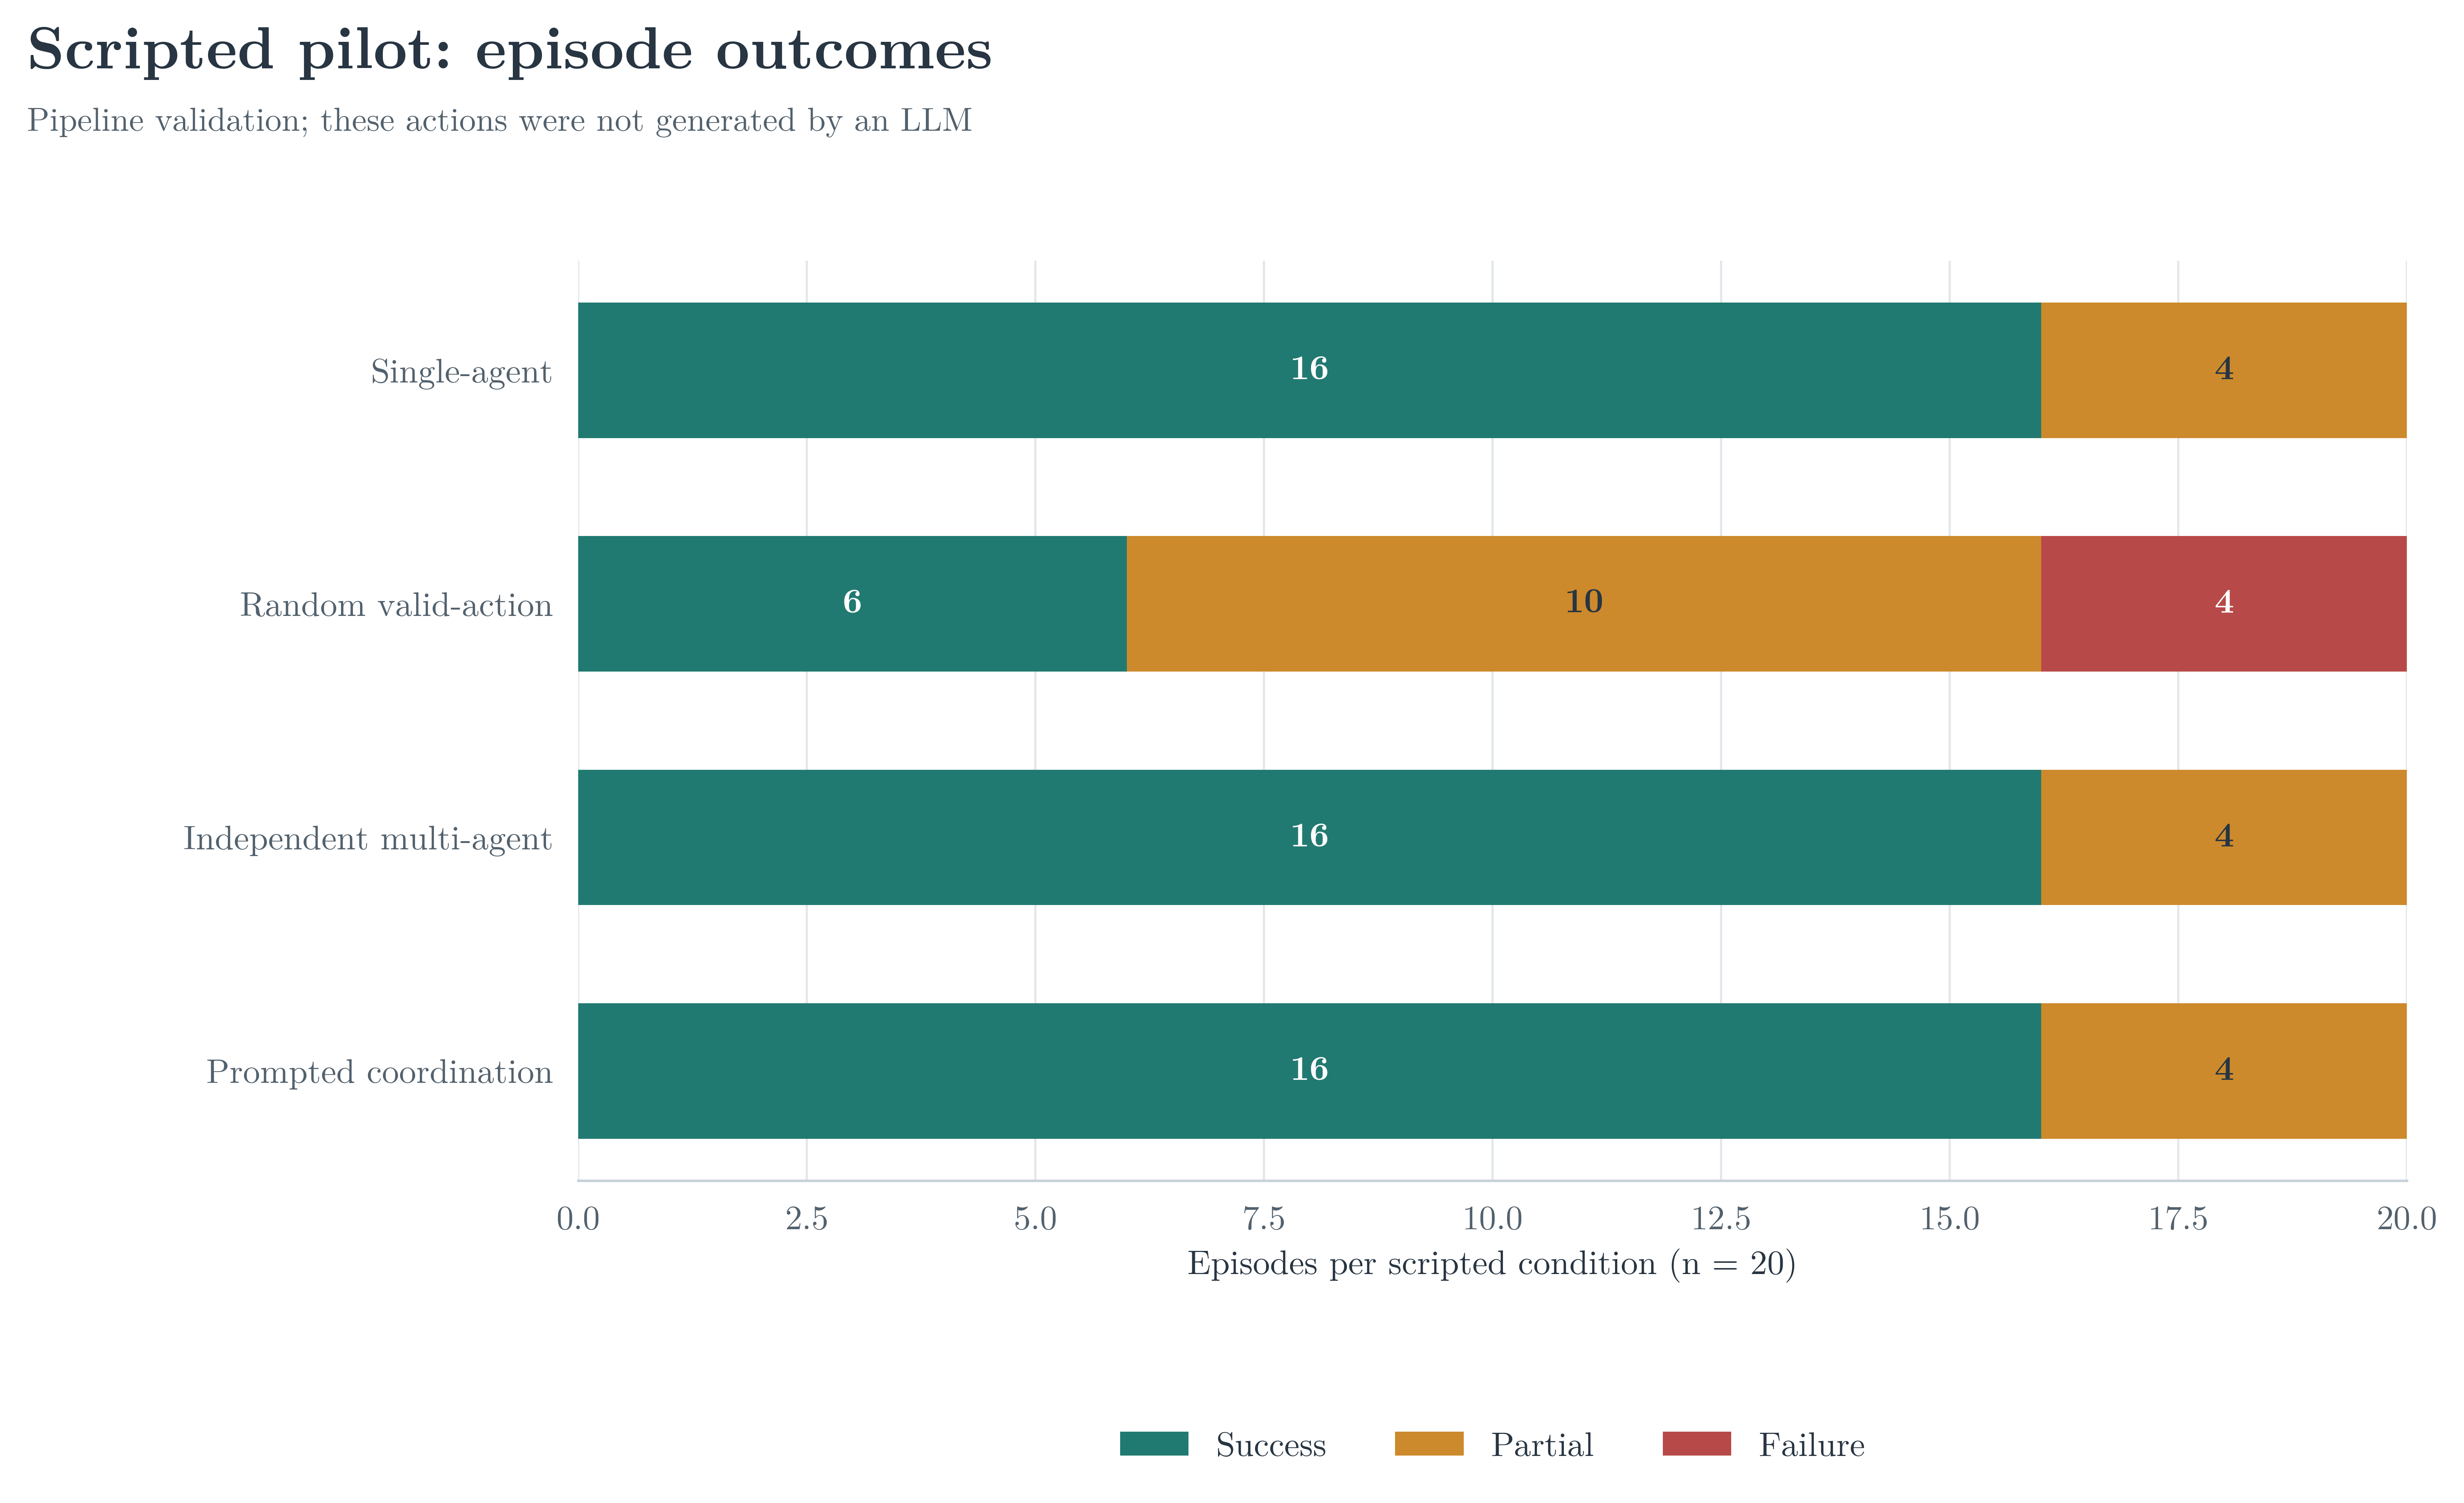
\includegraphics[width=\textwidth,height=0.68\textheight,keepaspectratio]{Images/08_scripted_pilot_outcomes.png}
\caption{Outcome counts from the 80-episode scripted pilot. These are baseline-policy results, separate from the later model-backed Phase 2 run.}
\label{figure:9}
\end{figure}
\section{Actions and scripted behavior}
The three non-random policies show the same observed aggregate tool sequence per episode: one \texttt{retrieve\allowbreak\_file}, one \texttt{search\allowbreak\_symbol}, two \texttt{apply\allowbreak\_patch} calls, two \texttt{run\allowbreak\_tests} calls, and one \texttt{finalize\allowbreak\_ticket} call. Each therefore records seven calls and 100\% patch acceptance. At the abstraction level, \texttt{retrieve\allowbreak\_file} and \texttt{search\allowbreak\_symbol} both map to \texttt{retrieve}; patches map to \texttt{update}, tests to \texttt{verify}, and finalization to \texttt{finalize}. Each such episode has two retrieve, two update, two verify, and one finalize event. Across each 20-episode condition this is 40 retrieve, 40 update, 40 verify, and 20 finalize events (definitions in \texttt{tool\allowbreak\_use\allowbreak\_environment.py}).

This matching pattern reflects the scripted plans, not an empirical discovery that multiple agents naturally converged on a useful division of work. \texttt{single\allowbreak\_agent} sets the episode to one agent; \texttt{independent\allowbreak\_multi\allowbreak\_agent} uses separate predefined per-agent action plans while turns advance sequentially; and \texttt{prompted\allowbreak\_coordination} follows a deterministic shared plan from \texttt{build\allowbreak\_demo\allowbreak\_actions()} (\texttt{tool\allowbreak\_use\allowbreak\_baselines.py}). In this scripted condition, “prompted” names the policy design; it is not a natural-language model prompt or an LLM intervention. The identical 16/4 outcomes and identical coarse action state for the two multi-agent policies provide no observed outcome or profile contrast between these policies in this run.

Random policy generated 126 calls across its 20 episodes: 28 retrievals, 28 symbol searches, 24 patch attempts, 35 test calls, and 11 finalizations. Its abstraction totals are 56 retrieve, 24 update, 35 verify, and 11 finalize, with no invalid-call category events. Unlike the fixed plans, it varies both action order and episode length. All four failures had zero fixed defects and averaged 3.5 calls, while the six successes averaged 7.67 calls; random episodes that failed could still contain valid calls and end through a valid but premature finalization. Its 20\% failure rate and lower success rate are descriptive for the sampled fixtures and policy seed behavior, not a general estimate for random agents or a causal benchmark against the other conditions.

\section{Coordination estimates and representation limits}
The saved \texttt{coordination\allowbreak\_report.json} estimates categorical mutual information between a joint pair of per-agent action representations and the episode outcome. Its primary representation, \texttt{coarsened\allowbreak\_action\allowbreak\_profile}, derives a per-agent category from action counts capped at two. It prioritizes \texttt{error\allowbreak\_or\allowbreak\_noop}, then \texttt{finalized}, \texttt{updated}, \texttt{verified}, \texttt{retrieved}, and \texttt{no\allowbreak\_actions}; this discards order and count detail to reduce cardinality (\texttt{coordination\allowbreak\_analysis.py}). The statistic is an empirical association in bits between encoded action profiles and \texttt{success}/\texttt{partial}/\texttt{failure}, not temporal information, causal effect, or the paper’s PID synergy.

For \texttt{random\allowbreak\_policy}, 17 of 20 episodes were eligible for a two-agent estimate; three were excluded because the event records did not contain actions from two distinct agents. On the 17 eligible episodes, the saved profile analysis has eight unique joint action-profile states and three observed outcomes, with plug-in MI of 0.83545 bits. The saved 95\% bootstrap interval is approximately [0.3083, 1.3590] bits, and its 250-permutation null reports \$p \textbackslash\{\}approx 0.1394\$. These diagnostics do not establish a reliable association in a larger population, much less that action profiles cause outcomes. With only 17 cases and multiple observed categories, sparse cells and finite-sample bias are substantial concerns.

The representation comparison makes this limitation concrete. \texttt{full\allowbreak\_trace} and capped \texttt{coarsened\allowbreak\_action\allowbreak\_counts} each distinguish 17 joint states among those 17 episodes and yield 1.37928 bits; \texttt{coarsened\allowbreak\_action\allowbreak\_profile} merges them to eight joint states and yields the lower value 0.83545 bits. The saved coordination artifact contains eight realized states. The validation tracker instead says nine profiles and quotes 1.04 bits, figures not supported by this run’s saved coordination artifact. Coarsening reduces the state space but does not validate that the six profile labels capture meaningful coordination or eliminate estimation bias.

For \texttt{independent\allowbreak\_multi\allowbreak\_agent} and \texttt{prompted\allowbreak\_coordination}, all 20 episodes are eligible but each condition has only one observed joint action-profile state. Outcomes are not literally constant: each condition has 16 successes and 4 partials. However, there are only two observed outcome categories and no failures, while the encoded joint action is constant; the saved MI is consequently 0 bits, with a zero-width bootstrap interval and permutation \$p=1\$. The outcome variation cannot be associated with a predictor that never varies. The one-agent condition is separately excluded from two-agent MI. Its report supplies a one-agent reference over 20 episodes, with one unique encoded action-profile state and 0 bits; it is not a two-agent coordination estimate. Accordingly, the validation tracker’s broad note that three baselines have “constant outcomes” is inaccurate if read literally. The important degeneracy here is the constant joint profile for the two scripted multi-agent policies and the restricted outcome support, not all-success episodes.

\section{Interpretation and limits}
The run demonstrates that, for these fixtures and policy implementations, the batch runner completed 80 episodes, retained per-episode summaries/events, reconciled its aggregate outcomes, and exported tables with an internally consistent count of 546 events. It also exercised the coordination pipeline across a policy with varied actions and outcomes and policies with highly repetitive action profiles. These are useful pipeline checks: they expose how encoding choice and category cardinality affect the saved statistic, and why a single MI value cannot stand in for a behavioral explanation.

The evidence remains exploratory for several reasons. The pilot contains only 20 episodes per scripted condition, uses a limited synthetic fixture/policy setup and an eight-call budget, and has no LLM-generated decisions despite the model name in its configuration. Three conditions share a fixed seven-action pattern; their matching rates do not demonstrate equivalence across other tasks or seeds. The random policy’s estimates are based on 17 eligible episodes and a high ratio of observed categories to observations. All tests are fixture rules rather than real program execution. The run therefore validates parts of the collection and analysis pipeline, not an external benchmark, a general ranking of multi-agent methods, or the paper’s account of emergence, synergy, complementarity, or goal-directed coordination. No conclusion should extend beyond these fixtures, scripted policies, and this 80-episode run.

\chapter{Phase 2: Model Pilots and Calibration}
\label{chapter-08}
\thispagestyle{plain}
Once the scripted pipeline was working, model-backed policies were added and small pilots were used to check response handling before the larger dataset was collected. These runs remain pre-final checks and are not pooled into the final experiment. The three early pilots each used one episode per policy on \texttt{math\allowbreak\_ops/offset\allowbreak\_scale}, seed 200. Calibration attempts are distinct; planned manifest size is not completed sample size.

\begin{table}[htbp]
\centering
\small
\setlength{\tabcolsep}{4pt}
\begin{tabularx}{\linewidth}{|Y|Y|Y|Y|}
\hline
\textbf{Run} & \textbf{Configured budget / mode} & \textbf{Completed episodes} & \textbf{Outcome by condition or key result} \\
\hline
Pilot A, 11 Sep & 8 calls; non-strict setting not recorded & 3 & Failure in all three policies; repeated retrieval, no patch or tests. \\
\hline
Pilot B, 11 Sep & 8 calls; non-strict setting not recorded & 3 & Partial in all three; one defect patched, one of two checks passed. \\
\hline
Pilot C, 11 Sep & 12 calls; non-strict setting not recorded & 3 & Success in all three; both defects patched and checks passed. \\
\hline
Calibration A, 12 Sep & Strict; 192 planned & 0 & First item failed after invalid structured responses; 191 pending. \\
\hline
Calibration B, 12 Sep & Strict; 192 planned & 0 & First item failed on response-format validation; 191 pending. \\
\hline
Preflight probe & Strict; 192 planned & 3 & One seed-200 \texttt{math\allowbreak\_ops/sum\allowbreak\_bounds} success per condition; 189 pending. \\
\hline
Thesis calibration slice & Strict; 192 planned & 3 & Same three condition/fixture instances completed successfully; 189 pending. \\
\hline
\end{tabularx}
\caption{Experiment runs and collection status}
\end{table}
The pilot sequence is not a controlled budget experiment: each budget occurred in a separate run with fresh model responses, and each policy has only one episode per run. The outcomes cannot isolate a causal budget effect or support policy ranking. The two failed calibration attempts surfaced structured-response failures before any completed episode; the later three-episode slices checked that strict-mode execution and artifacts could work, but they did not validate the full 192-item collection.

Before final collection, a paired 192-item design was adopted, with four repetitions over 16 fixture variants and strict fallback handling. The collection process also gained stronger manifest/progress checks, explicit retry/error records, artifact checks, and resume/retry selection. Final-run outcomes and retries are analyzed separately in Chapter 9; later maintenance should not be projected backward onto the earlier pilots.

\chapter{Phase 2: Final Experiment}
\label{chapter-09}
\thispagestyle{plain}
\section{Run design and scope}
The paired Phase 2 experiment analyzed in this chapter was run after the pilots and calibration checks. The analysis uses only the final run and does not pool earlier pilot or calibration data. The run uses the \texttt{synthetic\allowbreak\_bugfix} environment and the Azure AI deployment identified in its configuration as \texttt{azureai/gpt-5-mini}. Its three conditions are \texttt{llm\allowbreak\_single\allowbreak\_agent}, \texttt{llm\allowbreak\_independent\allowbreak\_multi\allowbreak\_agent}, and \texttt{llm\allowbreak\_prompted\allowbreak\_coordination}. The two multi-agent conditions use two agents; the single-agent policy uses one. Every episode has a 12-tool-call budget and strict LLM handling enabled (\texttt{experiment\allowbreak\_config.json}).

The manifest specifies 16 fixture variants, spanning eight task templates, with four repetitions in each condition-fixture cell. This yields 64 episodes per condition and 192 in total. Each fixture/repetition assignment is paired across the three conditions under a shared seed identity; the seed sequence begins at 200. The fixtures cover the configured arithmetic, string, retry-policy, flag-parsing, billing, scheduling, ranking, and inventory tasks. They are synthetic task instances: their test calls evaluate declared defect and regression state in the environment, not pytest, arbitrary source execution, or a real repository patch (\texttt{manifest.json}; \texttt{tool\allowbreak\_use\allowbreak\_environment.py}).

Independent enumeration confirms 192 unique manifest IDs and 192 unique summary IDs, with exact one-to-one coverage. There are 64 summaries for each condition and 12 manifest items per fixture variant across conditions. Every condition-fixture combination has one item at each repetition from one through four. The final \texttt{progress.json} records 192 completed, zero failed, zero pending, and \texttt{run\allowbreak\_complete=true}; \texttt{aggregate\allowbreak\_summary.json} agrees. These totals describe completed final episode artifacts, not the number of model or collection attempts.

\section{Episode outcomes}
The outcome table was recomputed by grouping the 192 episode-level \texttt{summary.json} files by condition and \texttt{outcome}. The results agree with both the aggregate and the saved quality-control table. \texttt{Partial} remains its own category: the five partial episodes are not counted as successes.

\begin{table}[htbp]
\centering
\small
\setlength{\tabcolsep}{4pt}
\begin{tabularx}{\linewidth}{|Y|Y|Y|Y|Y|}
\hline
\textbf{Condition} & \textbf{Episodes} & \textbf{Success} & \textbf{Partial} & \textbf{Failure} \\
\hline
\texttt{llm\allowbreak\_single\allowbreak\_agent} & 64 & 64 (100.00\%; 95\% Wilson CI: 94.34–100.00\%) & 0 (0.00\%) & 0 (0.00\%) \\
\hline
\texttt{llm\allowbreak\_independent\allowbreak\_multi\allowbreak\_agent} & 64 & 60 (93.75\%; 95\% Wilson CI: 85.00–97.54\%) & 4 (6.25\%) & 0 (0.00\%) \\
\hline
\texttt{llm\allowbreak\_prompted\allowbreak\_coordination} & 64 & 63 (98.44\%; 95\% Wilson CI: 91.67–99.72\%) & 1 (1.56\%) & 0 (0.00\%) \\
\hline
\textbf{Total} & \textbf{192} & \textbf{187 (97.40\%)} & \textbf{5 (2.60\%)} & \textbf{0 (0.00\%)} \\
\hline
\end{tabularx}
\caption{Final outcomes by policy condition}
\end{table}
\begin{figure}[htbp]
\centering
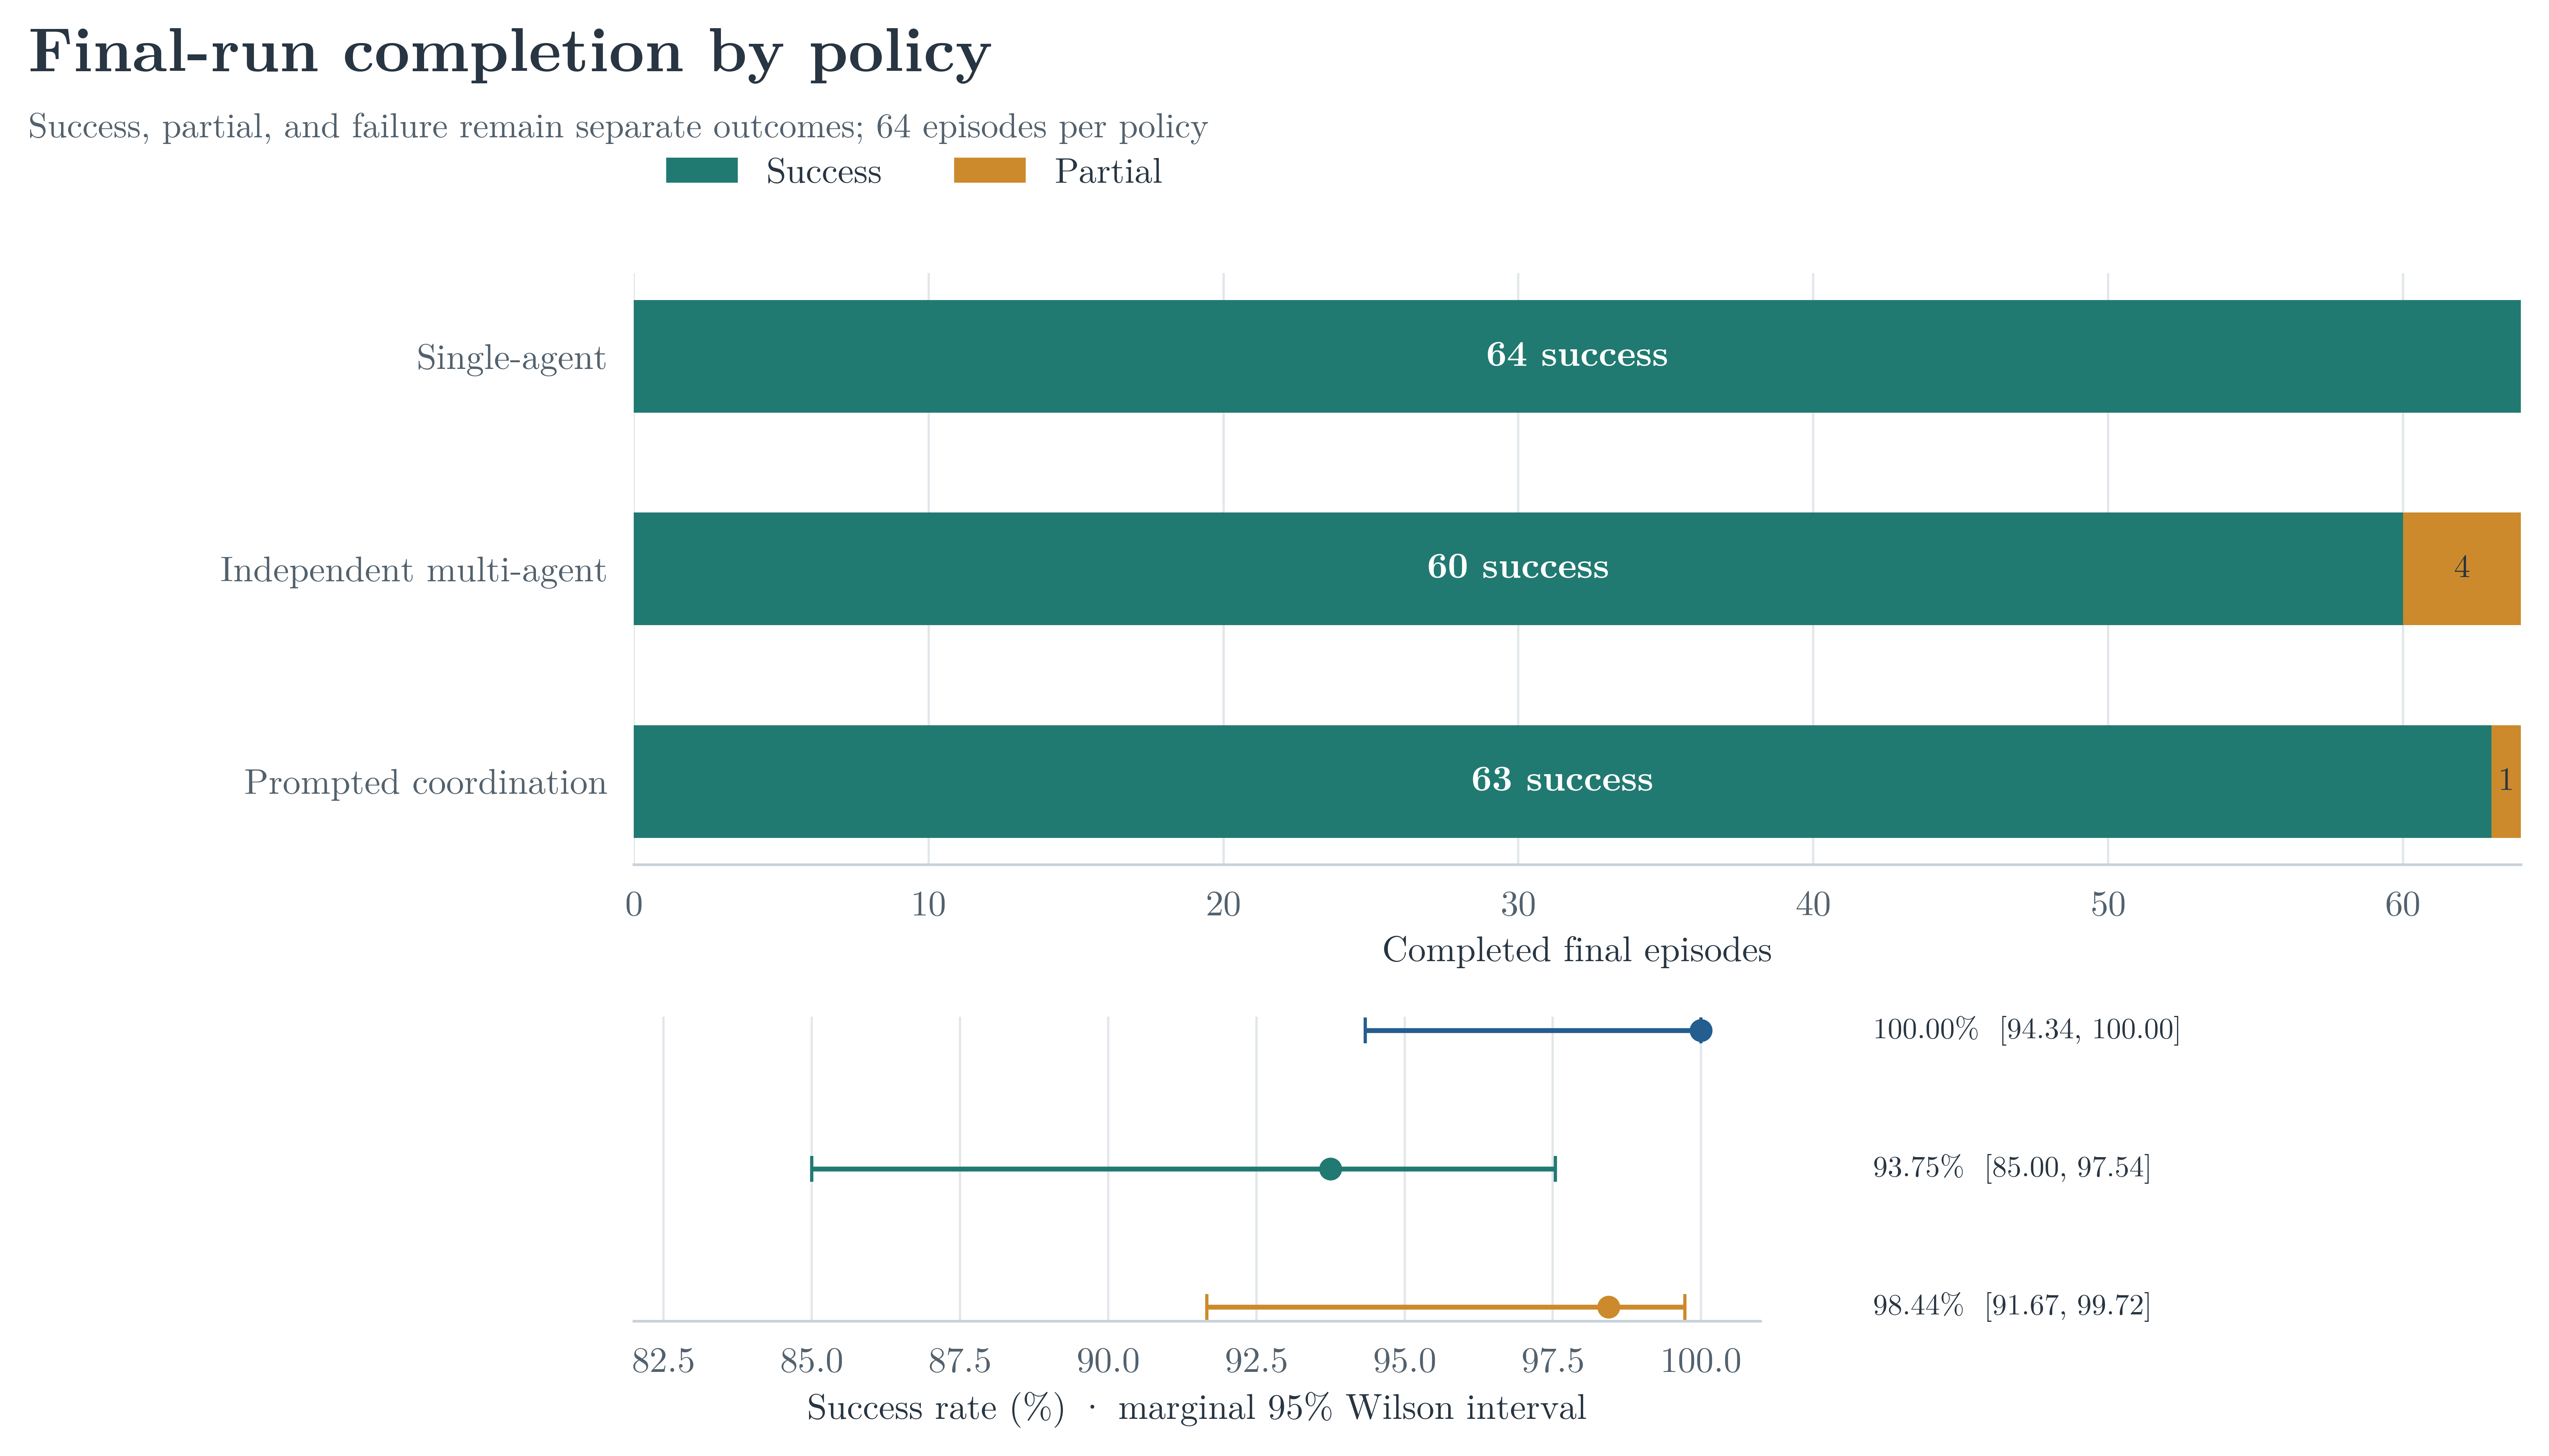
\includegraphics[width=\textwidth,height=0.68\textheight,keepaspectratio]{Images/09_final_outcomes.png}
\caption{Final-run outcomes across 192 completed episodes: 187 successes, five partials, and no failures. The five partial outcomes remain separate from successes.}
\label{figure:10}
\end{figure}
The marginal intervals are two-sided Wilson score intervals. Because the same 16 fixture variants and four repetitions were assigned to every condition, the paired contrasts below retain all three outcomes for each fixture/repetition assignment. The 95\% percentile intervals resample fixture variants as clusters (10,000 resamples; all four repetitions remain together within each sampled variant). These are effect-size and uncertainty summaries, not significance tests; the marginal Wilson intervals do not separately account for within-fixture dependence.

\begin{table}[htbp]
\centering
\small
\setlength{\tabcolsep}{4pt}
\begin{tabularx}{\linewidth}{|Y|Y|Y|}
\hline
\textbf{Paired contrast (A − B)} & \textbf{Success-rate difference (percentage points)} & \textbf{95\% fixture-cluster bootstrap interval} \\
\hline
Single-agent − independent multi-agent & +6.25 & [0.00, +15.62] \\
\hline
Single-agent − prompted coordination & +1.56 & [0.00, +4.69] \\
\hline
Prompted coordination − independent multi-agent & +4.69 & [0.00, +12.50] \\
\hline
\end{tabularx}
\caption{Paired condition contrasts in success rate}
\end{table}
The observed differences are small in absolute counts: single-agent has four more successes than independent multi-agent and one more than prompted coordination. The intervals describe uncertainty under this fixture-cluster resampling scheme; they do not establish superiority, equivalence, or a causal effect. The 16 fixture variants form an engineered catalog, not a random sample from a broader task population. The cluster bootstrap represents hypothetical re-sampling of these catalogued variants, keeping each variant's four repetitions together; it does not represent sampling uncertainty over a population of software tasks.

\begin{figure}[htbp]
\centering
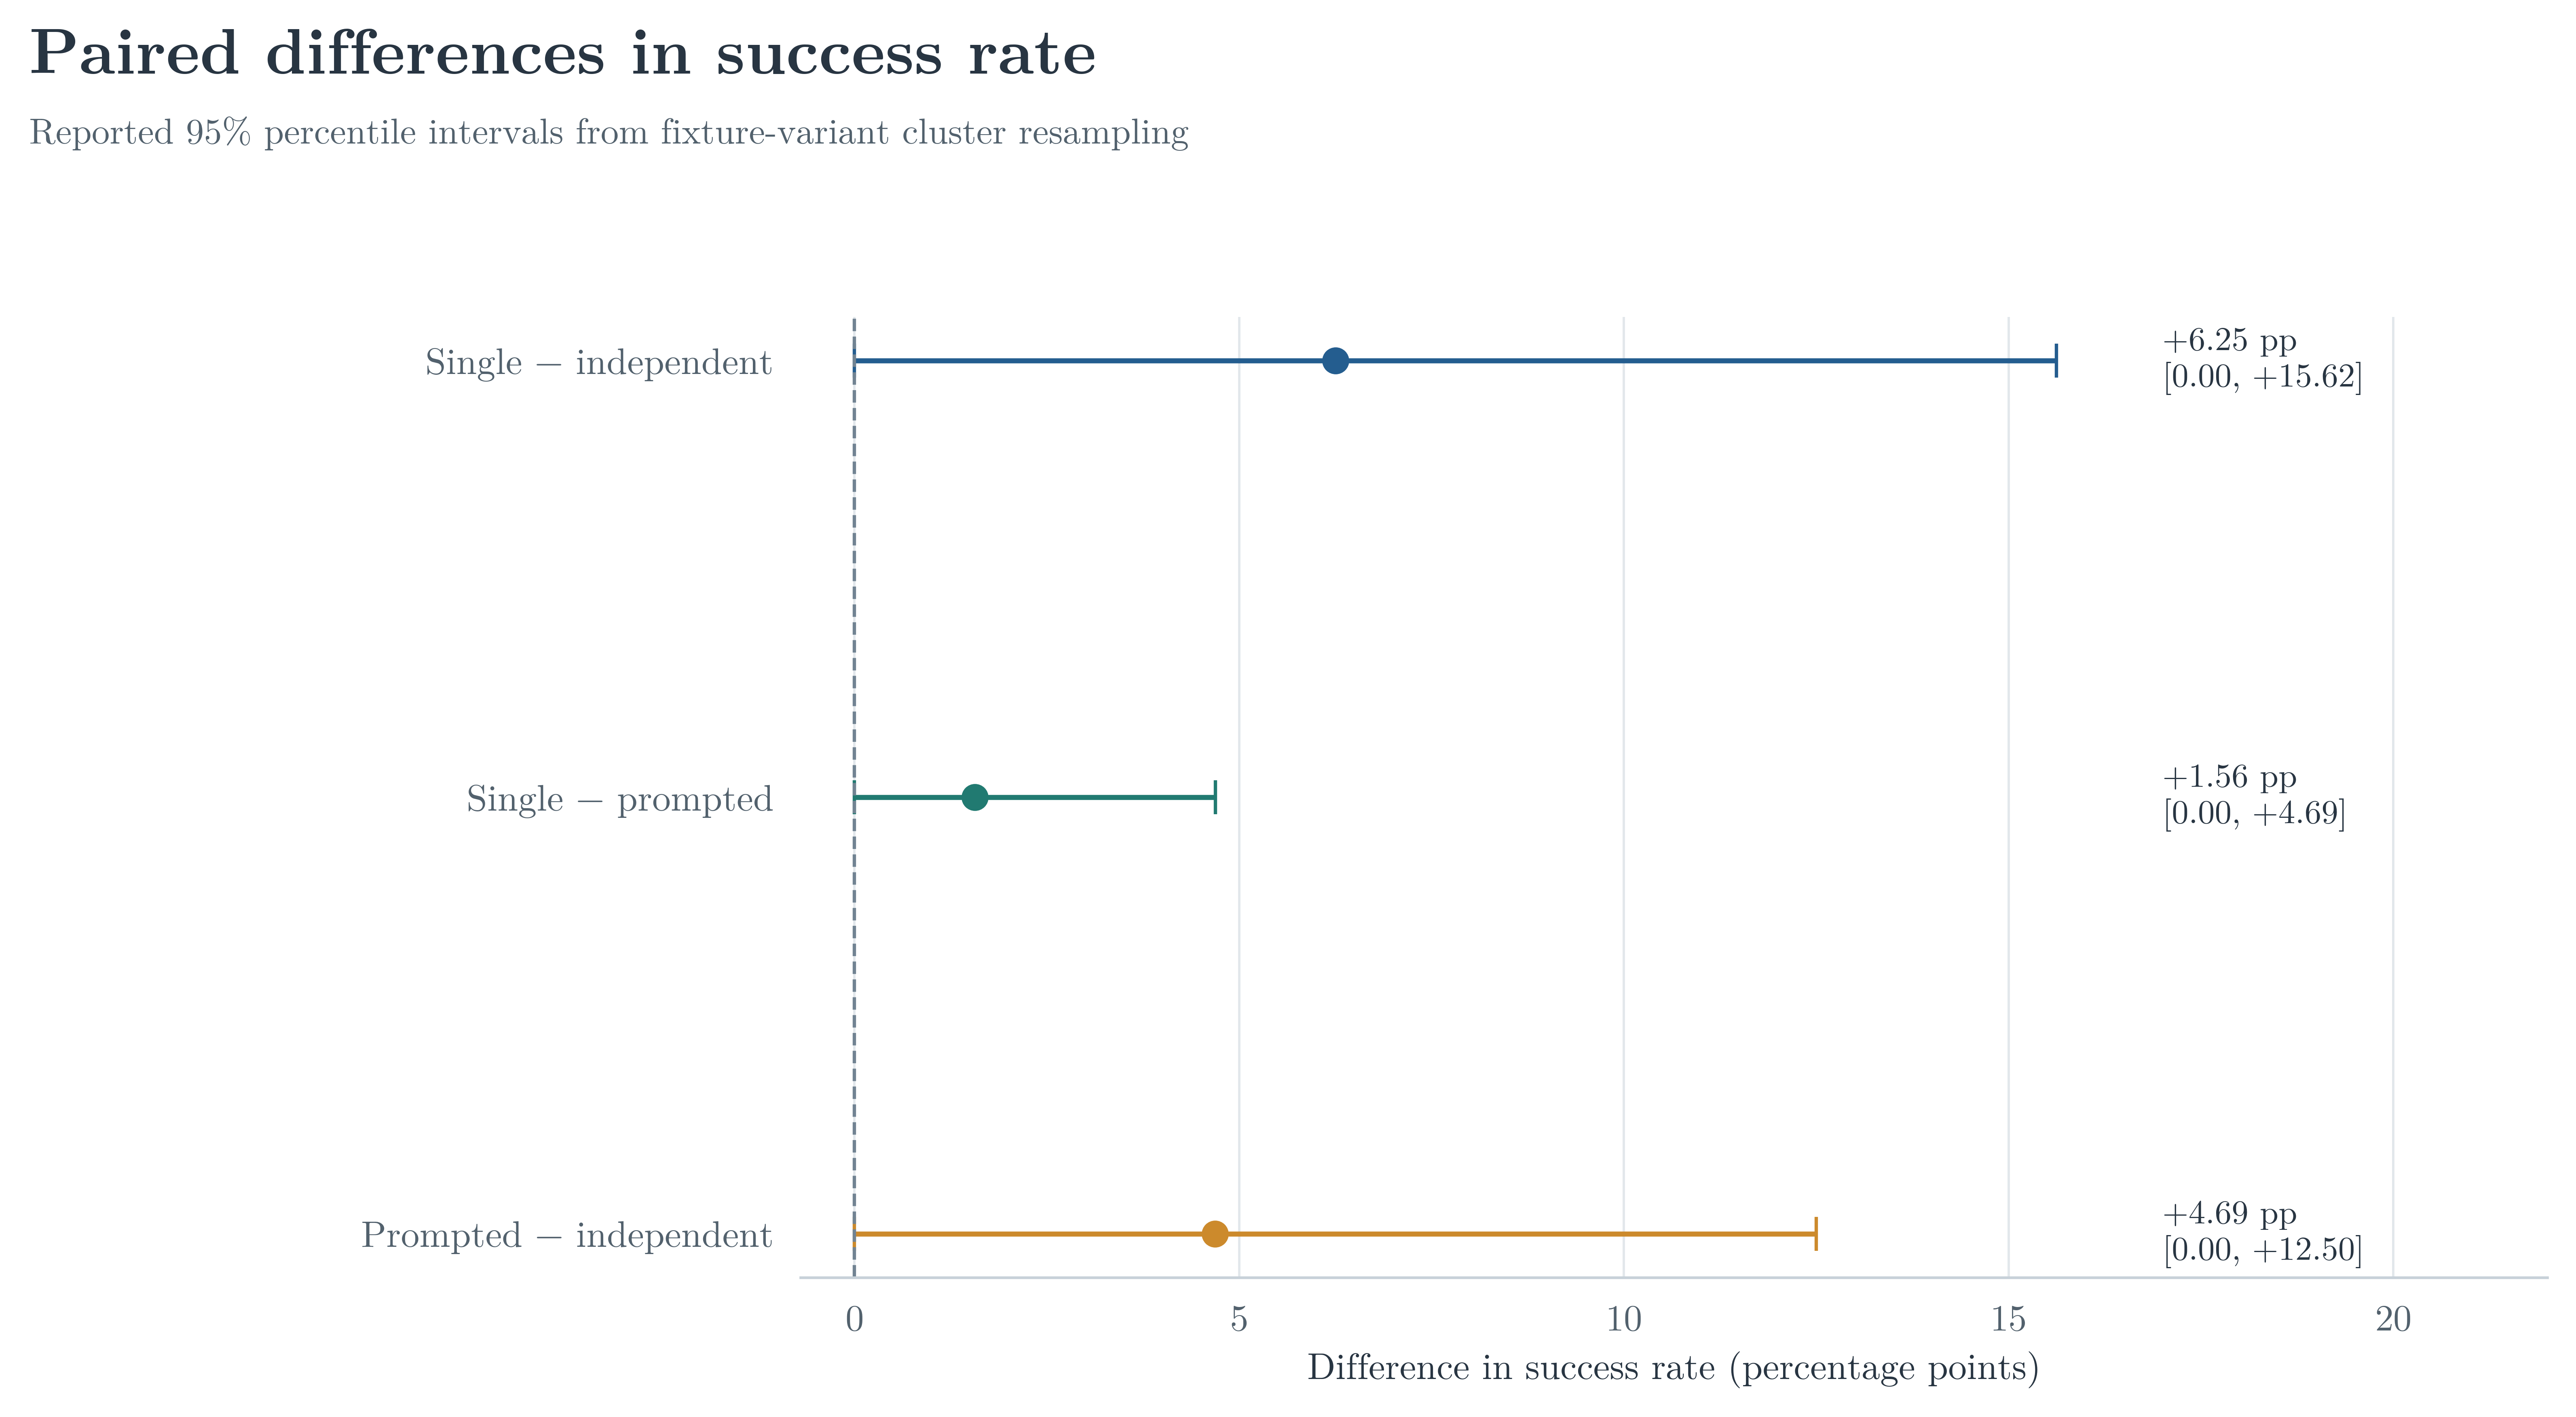
\includegraphics[width=\textwidth,height=0.68\textheight,keepaspectratio]{Images/10_paired_contrasts.png}
\caption{Paired success-rate differences and fixture-cluster bootstrap intervals. The intervals are descriptive uncertainty summaries, not significance tests or evidence of policy superiority.}
\label{figure:11}
\end{figure}
The environment assigns \texttt{partial} when at least some required-defect progress has been made but the fixture is not fully passing and no catastrophic regression has occurred; it is not a softer synonym for success. The four independent-policy partials and one coordinator partial therefore remain incomplete outcomes even though they are not failures. Conversely, zero failures means that no episode ended with the environment’s failure classification; it does not mean every episode reached full fixture completion, as the partial counts make clear. With success rates between 93.75\% and 100\%, the run also has limited outcome variation for distinguishing policies. This ceiling is relevant both to the descriptive outcome contrasts and to the later MI analysis, where only success and partial are observed.

\section{Examination of the five partial episodes}
To understand the incomplete outcomes, the five partial episodes' \texttt{episode.jsonl} action sequences and \texttt{summary.json} files were checked against their \texttt{task\allowbreak\_fixture.json} requirements. All five occur in the billing fixture family, and all end with a \texttt{finalize\allowbreak\_ticket} action before every required defect is fixed. None exhausted the 12-tool-call budget: the episodes finalized after four to six recorded calls. The grouped observations are:

\begin{table}[htbp]
\centering
\small
\setlength{\tabcolsep}{4pt}
\begin{tabularx}{\linewidth}{|Y|Y|Y|Y|}
\hline
\textbf{Fixture variant} & \textbf{Partial episodes by condition} & \textbf{Calls at finalization} & \textbf{Required defect still unresolved} \\
\hline
\texttt{billing/discount\allowbreak\_order} & 2 independent multi-agent & 5 and 6 & Primary defect; helper defect was fixed \\
\hline
\texttt{billing/invoice\allowbreak\_total} & 2 independent multi-agent; 1 prompted coordination & 5, 5, and 4 & Tertiary defect; primary and helper defects were fixed \\
\hline
\end{tabularx}
\caption{Partial episodes and unresolved defects}
\end{table}
Thus the direct, observable failure mode was \textbf{premature finalization with an incomplete fixture state}, not exhaustion of the available tool-call budget. For the same billing fixture/repetition assignments, the single-agent condition recorded success. This sharpens the descriptive single-agent versus multi-agent contrast, but it does not prove that agent count, coordination prompts, turn allocation, or any one model decision mechanism caused these partial outcomes. The saved traces show \emph{what} remained unfinished and \emph{when} the episodes terminated, not why the model selected finalization. Alongside the near-ceiling overall success rates, this case analysis suggests that stopping behavior and more discriminative task difficulty deserve closer attention in future evaluations. These observations were checked against the final run's per-episode traces and summaries.

\begin{figure}[htbp]
\centering
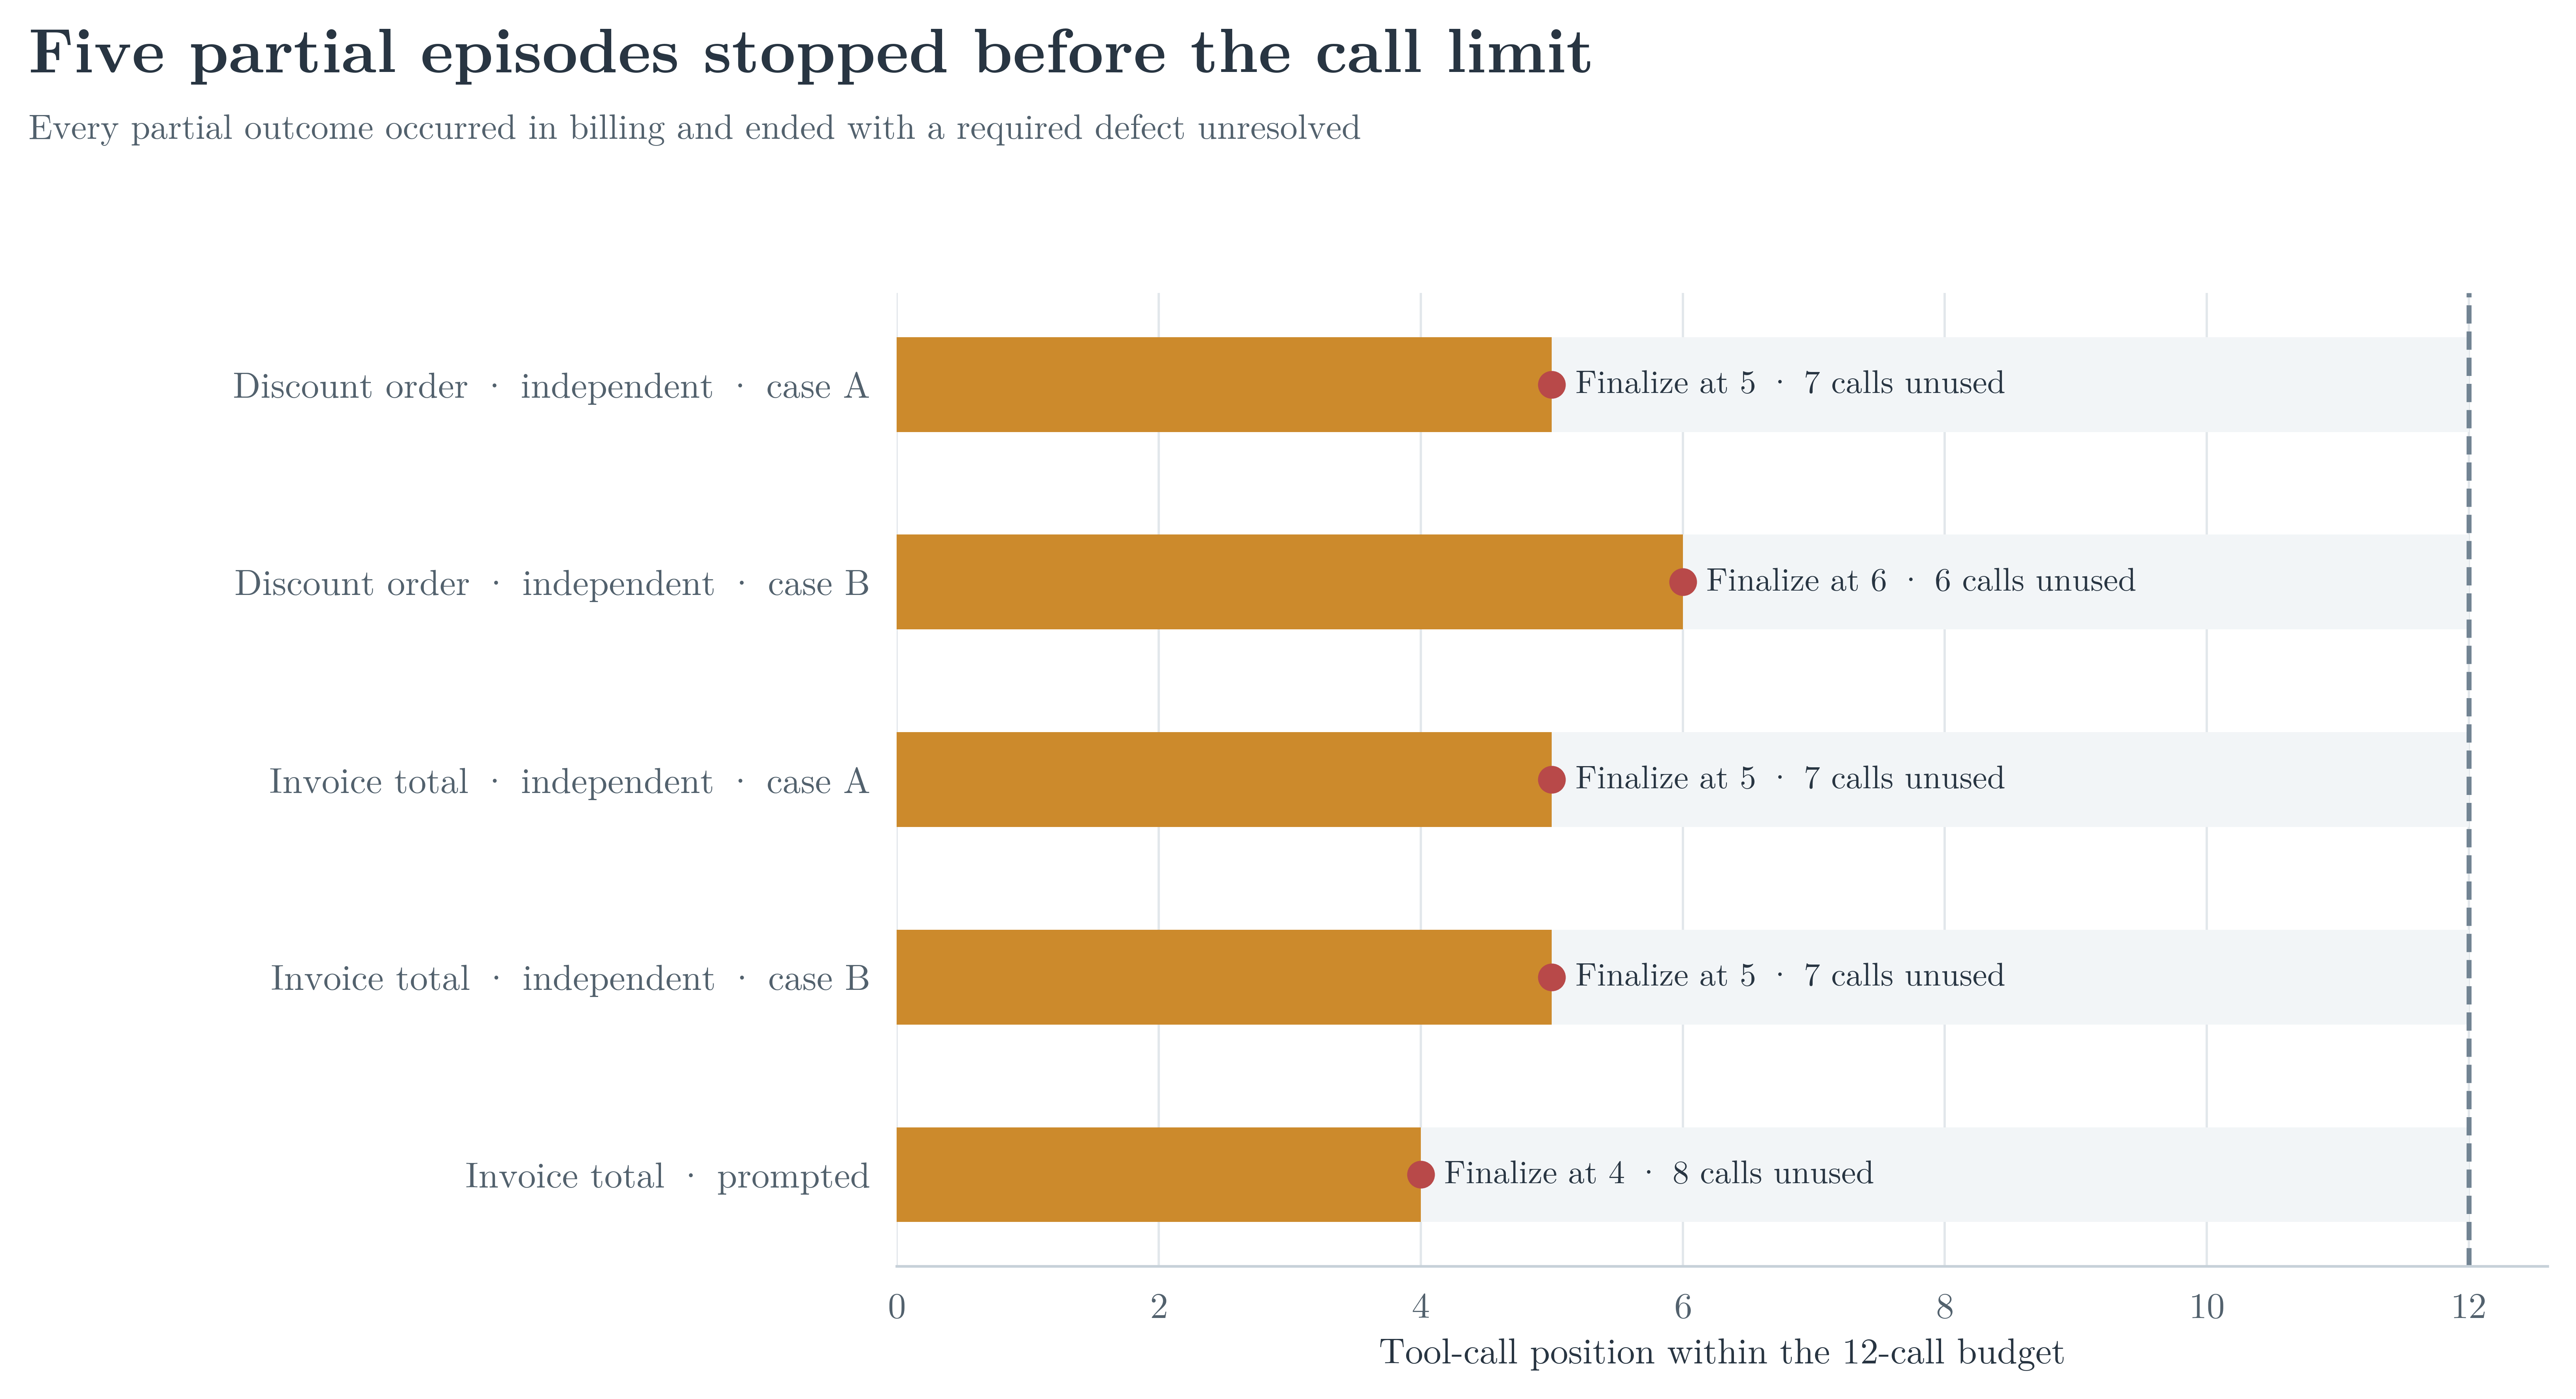
\includegraphics[width=\textwidth,height=0.68\textheight,keepaspectratio]{Images/12_premature_finalization.png}
\caption{The five partial episodes finalized before resolving all required defects; each retained tool-call budget. This visual summarizes the observed stopping pattern, not its cause.}
\label{figure:12}
\end{figure}
\section{Calls, patches, checks, and actions}
The 192 summaries report 1,181 tool events in total, matching the event rows counted in the JSONL traces and exports. Calls to completion count environment tool events, including finalization. The mean is 6.151 calls per episode overall. Condition-level calls, environment validity, patch acceptance, and test-call proportion are summarized below; the mean test-call proportion is the mean of per-episode fractions of calls that invoked \texttt{run\allowbreak\_tests}, not a ratio of pooled test calls to pooled actions (\texttt{aggregate\allowbreak\_summary.json}; \texttt{thesis\allowbreak\_results\allowbreak\_qc.md}).

\begin{table}[htbp]
\centering
\small
\setlength{\tabcolsep}{4pt}
\begin{tabularx}{\linewidth}{|Y|Y|Y|Y|Y|}
\hline
\textbf{Condition} & \textbf{Calls total / mean} & \textbf{Invalid-call rate} & \textbf{Accepted patches / attempts} & \textbf{Mean test-call proportion} \\
\hline
\texttt{llm\allowbreak\_single\allowbreak\_agent} & 416 / 6.5000 & 0.0000 & 136 / 136 (100\%) & 0.3230 \\
\hline
\texttt{llm\allowbreak\_independent\allowbreak\_multi\allowbreak\_agent} & 394 / 6.1563 & 0.0000 & 132 / 132 (100\%) & 0.2840 \\
\hline
\texttt{llm\allowbreak\_prompted\allowbreak\_coordination} & 371 / 5.7969 & 0.0000 & 135 / 135 (100\%) & 0.2697 \\
\hline
\textbf{Total} & \textbf{1,181 / 6.1510} & \textbf{0.0000} & \textbf{403 / 403 (100\%)} & — \\
\hline
\end{tabularx}
\caption{Tool-call and patch metrics by condition}
\end{table}
All 403 patch calls were accepted by the fixture environment, and there were no environment-invalid calls in any condition. Each of the five recorded invalid-call categories—\texttt{schema\allowbreak\_invalid}, \texttt{reference\allowbreak\_invalid}, \texttt{state\allowbreak\_invalid}, \texttt{semantic\allowbreak\_noop}, and \texttt{budget\allowbreak\_invalid}—has a total of zero. These perfect rates primarily describe the constrained interface documented in Section 5.2: prompts expose a dynamically filtered list of exact valid actions, including each recognized patch’s complete replacement text, and the environment accepts those catalog patches when their context remains present. They therefore measure selection and compliance within the supplied action space, not arbitrary patch generation or the quality of code changes. Moreover, the environment-invalid-call rate counts only submitted tool calls; the 96 invalid model responses that were recovered by retry occurred upstream and are recorded separately in Section 9.4. The two measures must not be conflated.

The saved tool counts also reconcile to 1,181. They show how action mix differed descriptively across the conditions:

\begin{table}[htbp]
\centering
\small
\setlength{\tabcolsep}{4pt}
\begin{tabularx}{\linewidth}{|Y|Y|Y|Y|Y|}
\hline
\textbf{Tool} & \textbf{Single agent} & \textbf{Independent multi-agent} & \textbf{Prompted coordination} & \textbf{Total} \\
\hline
\texttt{retrieve\allowbreak\_file} & 58 & 66 & 51 & 175 \\
\hline
\texttt{search\allowbreak\_symbol} & 25 & 19 & 21 & 65 \\
\hline
\texttt{apply\allowbreak\_patch} & 136 & 132 & 135 & 403 \\
\hline
\texttt{run\allowbreak\_tests} & 133 & 113 & 100 & 346 \\
\hline
\texttt{finalize\allowbreak\_ticket} & 64 & 64 & 64 & 192 \\
\hline
\textbf{All tool events} & \textbf{416} & \textbf{394} & \textbf{371} & \textbf{1,181} \\
\hline
\end{tabularx}
\caption{Tool-call totals by action type and condition}
\end{table}
At the coarser abstraction level used by the analysis, retrieval and symbol search combine into \texttt{retrieve}, patches become \texttt{update}, tests become \texttt{verify}, and finalization becomes \texttt{finalize}. Across the whole run these total 240 retrieve, 403 update, 346 verify, and 192 finalize events; there are no \texttt{error\allowbreak\_or\allowbreak\_noop} events. The fixed patch acceptance and lack of invalid actions are properties of the submitted calls and environment validator. They do not show that all policies made the same decisions: the tool distributions differ, and the event order and acting-agent assignment also vary. Nor does a shorter mean action sequence by itself establish greater efficiency, because the outcomes and task states must be considered alongside it.

\begin{figure}[htbp]
\centering
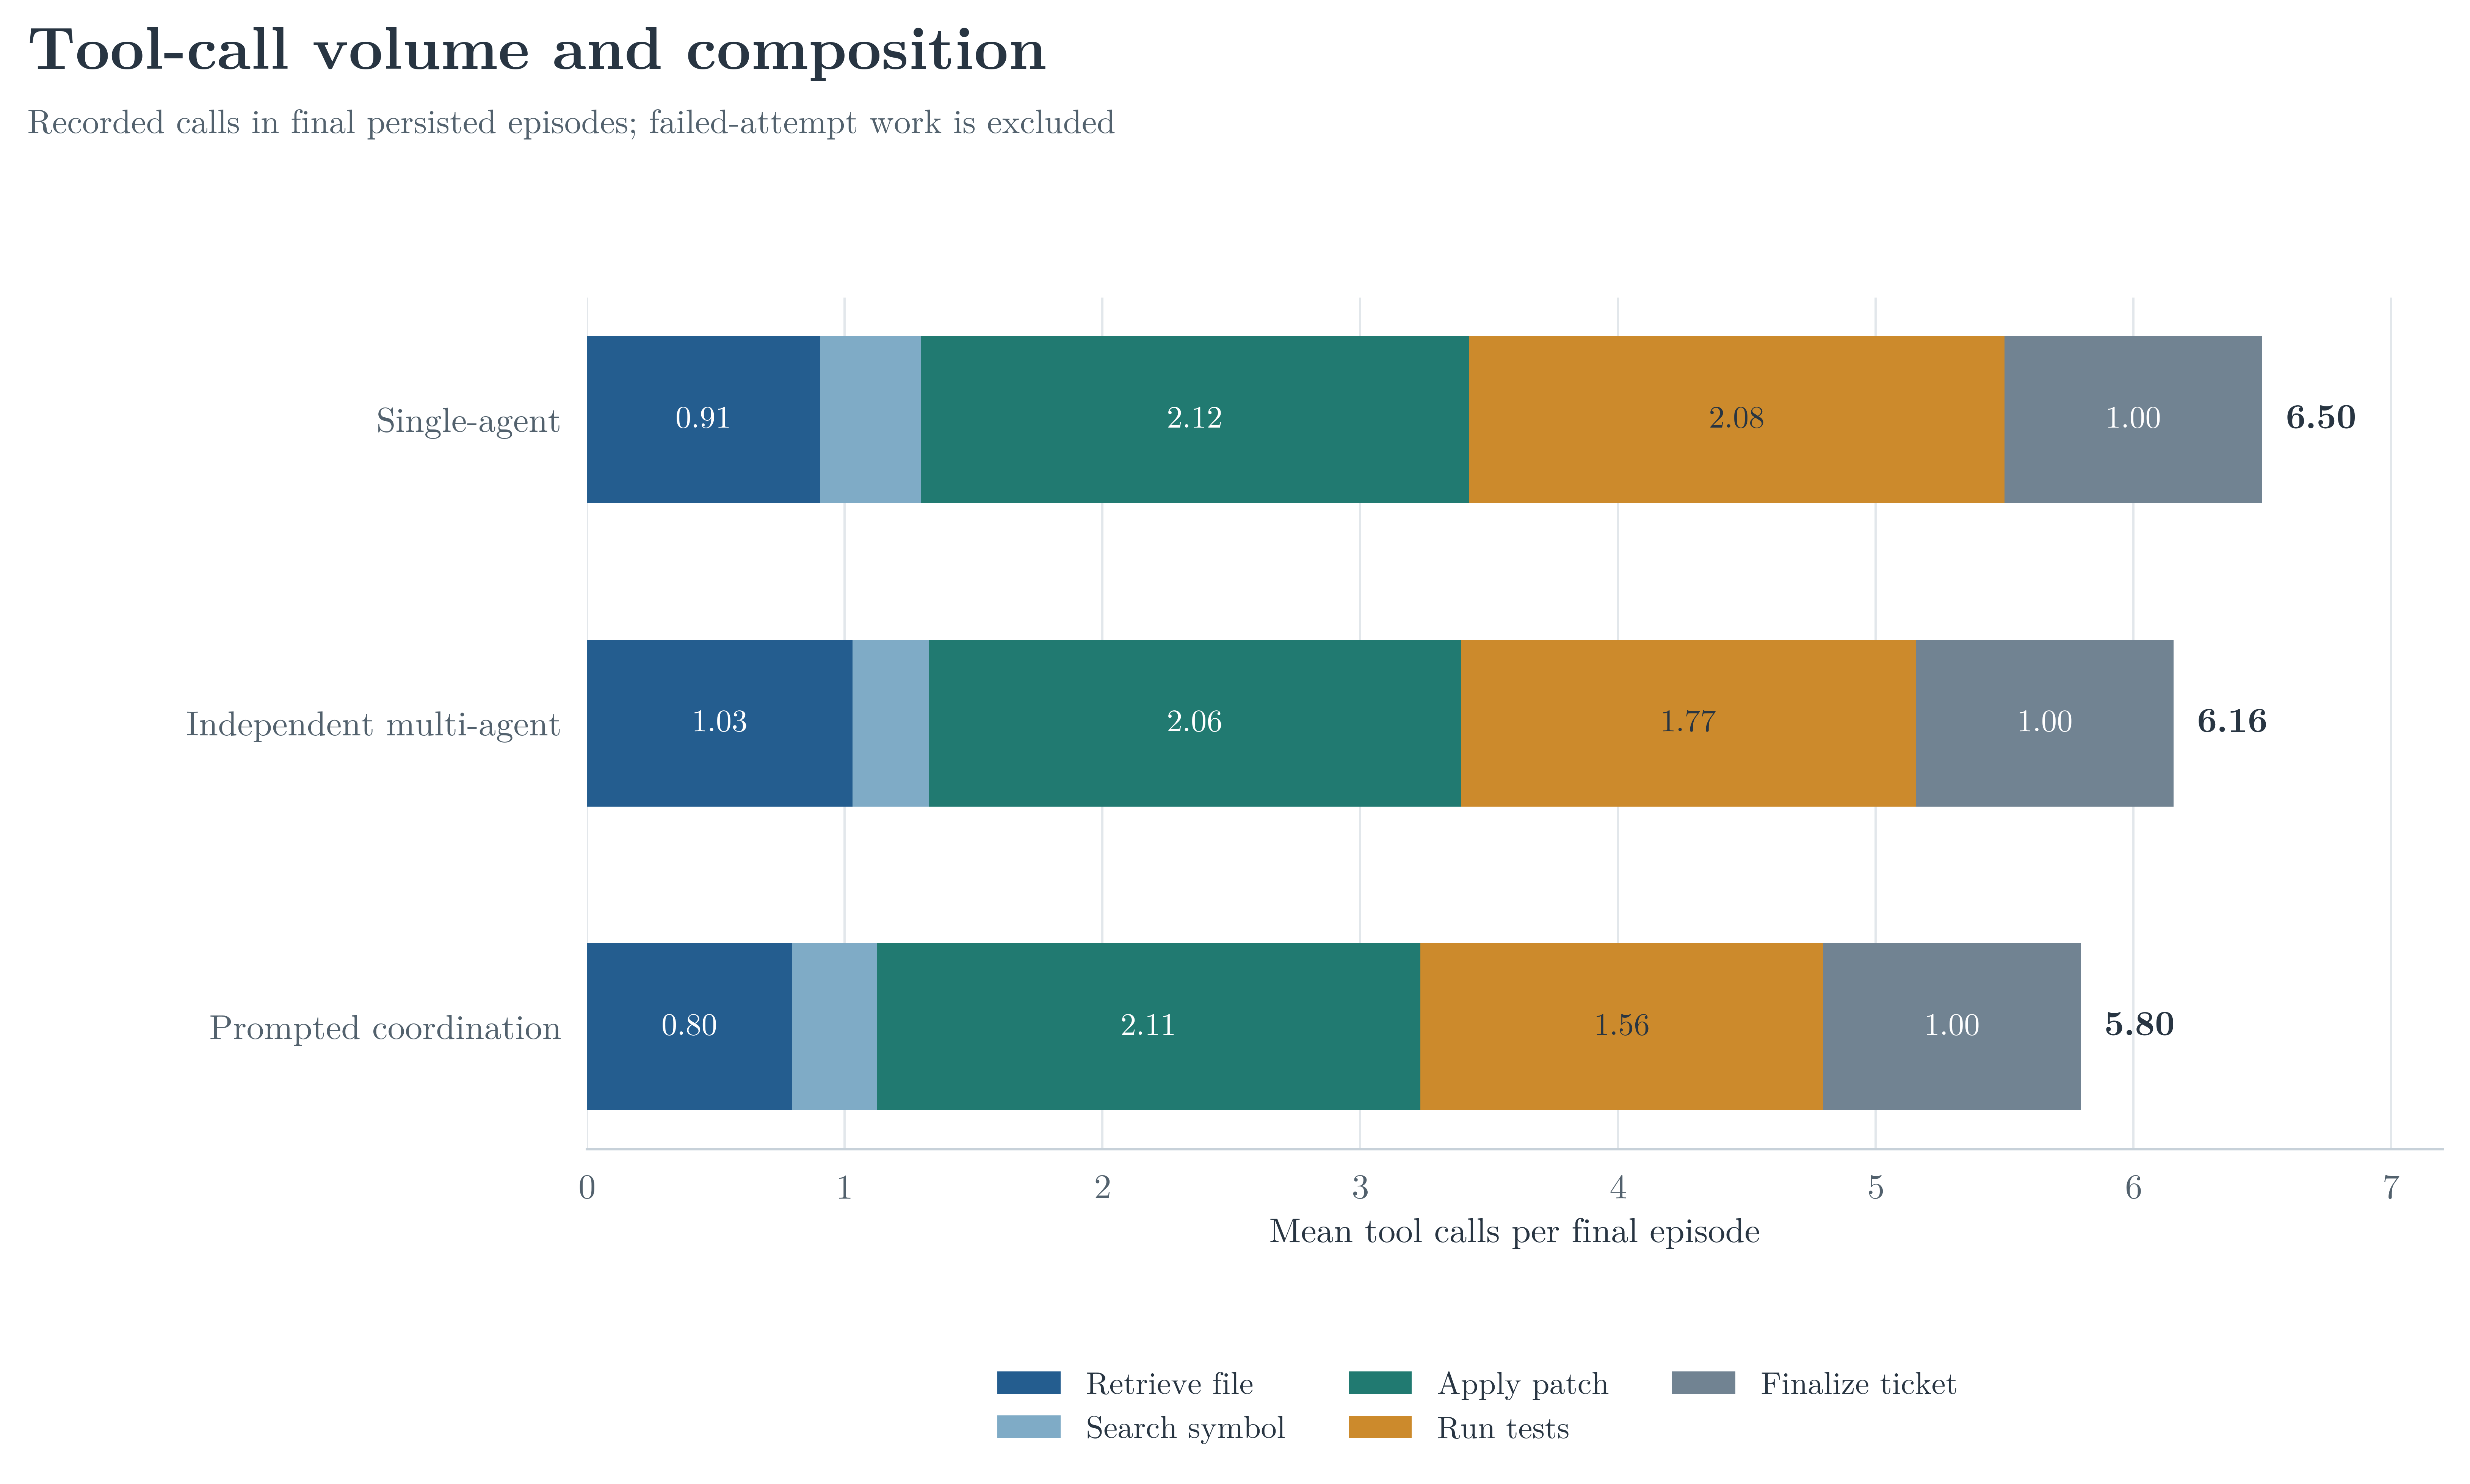
\includegraphics[width=\textwidth,height=0.68\textheight,keepaspectratio]{Images/11_tool_call_mix.png}
\caption{Recorded tool-call totals by condition. Differences describe the saved traces and should be interpreted together with outcomes and task state, not as standalone efficiency scores.}
\label{figure:13}
\end{figure}
\section{Response validation and retry history}
The episode-level policy audits record 96 recoverable invalid model responses across 81 final episodes: 34 responses in 26 single-agent episodes, 35 in 30 independent multi-agent episodes, and 27 in 25 prompted-coordination episodes. These are parsing/action-validation issues that were recovered during the final episode’s policy loop; they are not invalid environment tool calls. In the same completed summaries, strict audit records zero fallback responses, zero locally selected fallback actions, and zero model-call errors. Thus the final action traces contain no recorded soft-fallback actions even though some model outputs required another attempt (\texttt{thesis\allowbreak\_results\allowbreak\_qc.md}).

The final run recorded 56 episode-error records, all typed \texttt{LLMResponseError}, classified retryable, and marked \texttt{retryable=true}. They concern 23 unique manifest IDs; independently, each of those IDs is present among the 192 final summaries. The records describe attempts where an invalid response/action remained after two policy parse attempts. The final rejection reasons were: failure to match a currently valid action (42 records), a repeated action that should not be repeated (13), and a response with a non-string \texttt{tool\allowbreak\_name} or non-object \texttt{arguments} (one). Some IDs have several error records, reflecting repeated failed attempts before a successful completion; the most-retried ID has nine error records.

\textbf{Retry semantics and first-attempt completion.} A collection retry reruns the entire manifest episode from its start with the same frozen seed and fixture; it does not resume at the interrupted action. The runner calls the episode policy again, which constructs a fresh environment and event sequence. \texttt{--retry-failures} requires resuming the existing run directory and selects manifest items currently marked failed; already completed IDs are skipped. The initial 192-item sweep completed 169 episodes and failed 23. Every initially failed ID subsequently completed. The table separates first-pass task observations from the failed technical attempts:

\begin{table}[htbp]
\centering
\small
\setlength{\tabcolsep}{4pt}
\begin{tabularx}{\linewidth}{|Y|Y|Y|Y|Y|Y|}
\hline
\textbf{Condition} & \textbf{Completed on first attempt} & \textbf{Failed on first attempt / affected IDs} & \textbf{Failed-attempt records} & \textbf{Additional failed retries after first attempt} & \textbf{Affected IDs eventually completed} \\
\hline
\texttt{llm\allowbreak\_single\allowbreak\_agent} & 57 / 64 & 7 & 18 & 11 & 7 / 7 \\
\hline
\texttt{llm\allowbreak\_independent\allowbreak\_multi\allowbreak\_agent} & 53 / 64 & 11 & 27 & 16 & 11 / 11 \\
\hline
\texttt{llm\allowbreak\_prompted\allowbreak\_coordination} & 59 / 64 & 5 & 11 & 6 & 5 / 5 \\
\hline
\textbf{Total} & \textbf{169 / 192} & \textbf{23} & \textbf{56} & \textbf{33} & \textbf{23 / 23} \\
\hline
\end{tabularx}
\caption{Response recovery and collection retry summary}
\end{table}
The 56 records comprise 23 failures on the first pass and 33 further failed whole-episode attempts. The 23 affected IDs each then had one successful rerun, so the run involved \textbf{56 whole-episode retries} and \textbf{248 episode executions in total} (192 initial executions plus 56 reruns). The runner has no automatic episode-retry cap: retrying is an explicit resume operation, and failed IDs can be selected again in another invocation. This is distinct from the two policy parse attempts allowed for an invalid action response. The largest observed count was nine failed attempts for one ID; it is an observed maximum, not a configured limit.

The final outcome table uses one eventually technically completed trace per manifest ID; it is not the outcome distribution from a uniformly capped first-pass protocol. Since response-validity failures may be related to fixture or policy behavior, whole-episode restarts can affect which trajectories are retained. This is a selection limit on the observed traces, not a reason to reclassify technical collection failures as task failures.

Affected manifest IDs and the number of failed collection attempts recorded for each are:

\begin{itemize}
\item \texttt{llm\allowbreak\_single\allowbreak\_agent}: \texttt{llm\allowbreak\_single\allowbreak\_agent\allowbreak\_\allowbreak\_rep\allowbreak\_001\allowbreak\_\allowbreak\_seed\allowbreak\_212\allowbreak\_\allowbreak\_string\allowbreak\_utils\allowbreak\_\allowbreak\_slugify} (1); \texttt{llm\allowbreak\_single\allowbreak\_agent\allowbreak\_\allowbreak\_rep\allowbreak\_001\allowbreak\_\allowbreak\_seed\allowbreak\_216\allowbreak\_\allowbreak\_retry\allowbreak\_policy\allowbreak\_\allowbreak\_max\allowbreak\_attempts} (1); \texttt{llm\allowbreak\_single\allowbreak\_agent\allowbreak\_\allowbreak\_rep\allowbreak\_001\allowbreak\_\allowbreak\_seed\allowbreak\_232\allowbreak\_\allowbreak\_billing\allowbreak\_\allowbreak\_discount\allowbreak\_order} (5); \texttt{llm\allowbreak\_single\allowbreak\_agent\allowbreak\_\allowbreak\_rep\allowbreak\_002\allowbreak\_\allowbreak\_seed\allowbreak\_213\allowbreak\_\allowbreak\_string\allowbreak\_utils\allowbreak\_\allowbreak\_slugify} (2); \texttt{llm\allowbreak\_single\allowbreak\_agent\allowbreak\_\allowbreak\_rep\allowbreak\_003\allowbreak\_\allowbreak\_seed\allowbreak\_234\allowbreak\_\allowbreak\_billing\allowbreak\_\allowbreak\_discount\allowbreak\_order} (1); \texttt{llm\allowbreak\_single\allowbreak\_agent\allowbreak\_\allowbreak\_rep\allowbreak\_004\allowbreak\_\allowbreak\_seed\allowbreak\_215\allowbreak\_\allowbreak\_string\allowbreak\_utils\allowbreak\_\allowbreak\_slugify} (7); \texttt{llm\allowbreak\_single\allowbreak\_agent\allowbreak\_\allowbreak\_rep\allowbreak\_004\allowbreak\_\allowbreak\_seed\allowbreak\_235\allowbreak\_\allowbreak\_billing\allowbreak\_\allowbreak\_discount\allowbreak\_order} (1).
\item \texttt{llm\allowbreak\_independent\allowbreak\_multi\allowbreak\_agent}: \texttt{llm\allowbreak\_independent\allowbreak\_multi\allowbreak\_agent\allowbreak\_\allowbreak\_rep\allowbreak\_001\allowbreak\_\allowbreak\_seed\allowbreak\_212\allowbreak\_\allowbreak\_string\allowbreak\_utils\allowbreak\_\allowbreak\_slugify} (2); \texttt{llm\allowbreak\_independent\allowbreak\_multi\allowbreak\_agent\allowbreak\_\allowbreak\_rep\allowbreak\_002\allowbreak\_\allowbreak\_seed\allowbreak\_213\allowbreak\_\allowbreak\_string\allowbreak\_utils\allowbreak\_\allowbreak\_slugify} (3); \texttt{llm\allowbreak\_independent\allowbreak\_multi\allowbreak\_agent\allowbreak\_\allowbreak\_rep\allowbreak\_002\allowbreak\_\allowbreak\_seed\allowbreak\_257\allowbreak\_\allowbreak\_inventory\allowbreak\_\allowbreak\_stock\allowbreak\_count} (1); \texttt{llm\allowbreak\_independent\allowbreak\_multi\allowbreak\_agent\allowbreak\_\allowbreak\_rep\allowbreak\_003\allowbreak\_\allowbreak\_seed\allowbreak\_214\allowbreak\_\allowbreak\_string\allowbreak\_utils\allowbreak\_\allowbreak\_slugify} (1); \texttt{llm\allowbreak\_independent\allowbreak\_multi\allowbreak\_agent\allowbreak\_\allowbreak\_rep\allowbreak\_003\allowbreak\_\allowbreak\_seed\allowbreak\_218\allowbreak\_\allowbreak\_retry\allowbreak\_policy\allowbreak\_\allowbreak\_max\allowbreak\_attempts} (1); \texttt{llm\allowbreak\_independent\allowbreak\_multi\allowbreak\_agent\allowbreak\_\allowbreak\_rep\allowbreak\_003\allowbreak\_\allowbreak\_seed\allowbreak\_234\allowbreak\_\allowbreak\_billing\allowbreak\_\allowbreak\_discount\allowbreak\_order} (2); \texttt{llm\allowbreak\_independent\allowbreak\_multi\allowbreak\_agent\allowbreak\_\allowbreak\_rep\allowbreak\_004\allowbreak\_\allowbreak\_seed\allowbreak\_203\allowbreak\_\allowbreak\_math\allowbreak\_ops\allowbreak\_\allowbreak\_sum\allowbreak\_bounds} (1); \texttt{llm\allowbreak\_independent\allowbreak\_multi\allowbreak\_agent\allowbreak\_\allowbreak\_rep\allowbreak\_004\allowbreak\_\allowbreak\_seed\allowbreak\_215\allowbreak\_\allowbreak\_string\allowbreak\_utils\allowbreak\_\allowbreak\_slugify} (9); \texttt{llm\allowbreak\_independent\allowbreak\_multi\allowbreak\_agent\allowbreak\_\allowbreak\_rep\allowbreak\_004\allowbreak\_\allowbreak\_seed\allowbreak\_235\allowbreak\_\allowbreak\_billing\allowbreak\_\allowbreak\_discount\allowbreak\_order} (1); \texttt{llm\allowbreak\_independent\allowbreak\_multi\allowbreak\_agent\allowbreak\_\allowbreak\_rep\allowbreak\_004\allowbreak\_\allowbreak\_seed\allowbreak\_259\allowbreak\_\allowbreak\_inventory\allowbreak\_\allowbreak\_stock\allowbreak\_count} (5); \texttt{llm\allowbreak\_independent\allowbreak\_multi\allowbreak\_agent\allowbreak\_\allowbreak\_rep\allowbreak\_004\allowbreak\_\allowbreak\_seed\allowbreak\_263\allowbreak\_\allowbreak\_inventory\allowbreak\_\allowbreak\_reserve\allowbreak\_logic} (1).
\item \texttt{llm\allowbreak\_prompted\allowbreak\_coordination}: \texttt{llm\allowbreak\_prompted\allowbreak\_coordination\allowbreak\_\allowbreak\_rep\allowbreak\_001\allowbreak\_\allowbreak\_seed\allowbreak\_212\allowbreak\_\allowbreak\_string\allowbreak\_utils\allowbreak\_\allowbreak\_slugify} (4); \texttt{llm\allowbreak\_prompted\allowbreak\_coordination\allowbreak\_\allowbreak\_rep\allowbreak\_001\allowbreak\_\allowbreak\_seed\allowbreak\_216\allowbreak\_\allowbreak\_retry\allowbreak\_policy\allowbreak\_\allowbreak\_max\allowbreak\_attempts} (1); \texttt{llm\allowbreak\_prompted\allowbreak\_coordination\allowbreak\_\allowbreak\_rep\allowbreak\_002\allowbreak\_\allowbreak\_seed\allowbreak\_213\allowbreak\_\allowbreak\_string\allowbreak\_utils\allowbreak\_\allowbreak\_slugify} (2); \texttt{llm\allowbreak\_prompted\allowbreak\_coordination\allowbreak\_\allowbreak\_rep\allowbreak\_002\allowbreak\_\allowbreak\_seed\allowbreak\_233\allowbreak\_\allowbreak\_billing\allowbreak\_\allowbreak\_discount\allowbreak\_order} (3); \texttt{llm\allowbreak\_prompted\allowbreak\_coordination\allowbreak\_\allowbreak\_rep\allowbreak\_004\allowbreak\_\allowbreak\_seed\allowbreak\_235\allowbreak\_\allowbreak\_billing\allowbreak\_\allowbreak\_discount\allowbreak\_order} (1).
\end{itemize}
These counts describe technical collection reliability, not task performance. An error artifact has no completed environment outcome; a manifest ID contributes at most one final summary to the 192-episode outcome table. Likewise, the 1,181 accepted tool events count only the final persisted traces, not work performed in failed attempts. The saved run does not record token usage, complete model-request totals, per-attempt duration, or provider billing, so a monetary/API-usage collection cost cannot be reconstructed. The observable retry burden is the 56 full-episode reruns above. The response-validation counts in the failed-attempt artifacts describe those attempts and should not be added to the 96 recoverable invalid responses in the final summaries as though they were final-episode outcomes.

\begin{figure}[htbp]
\centering
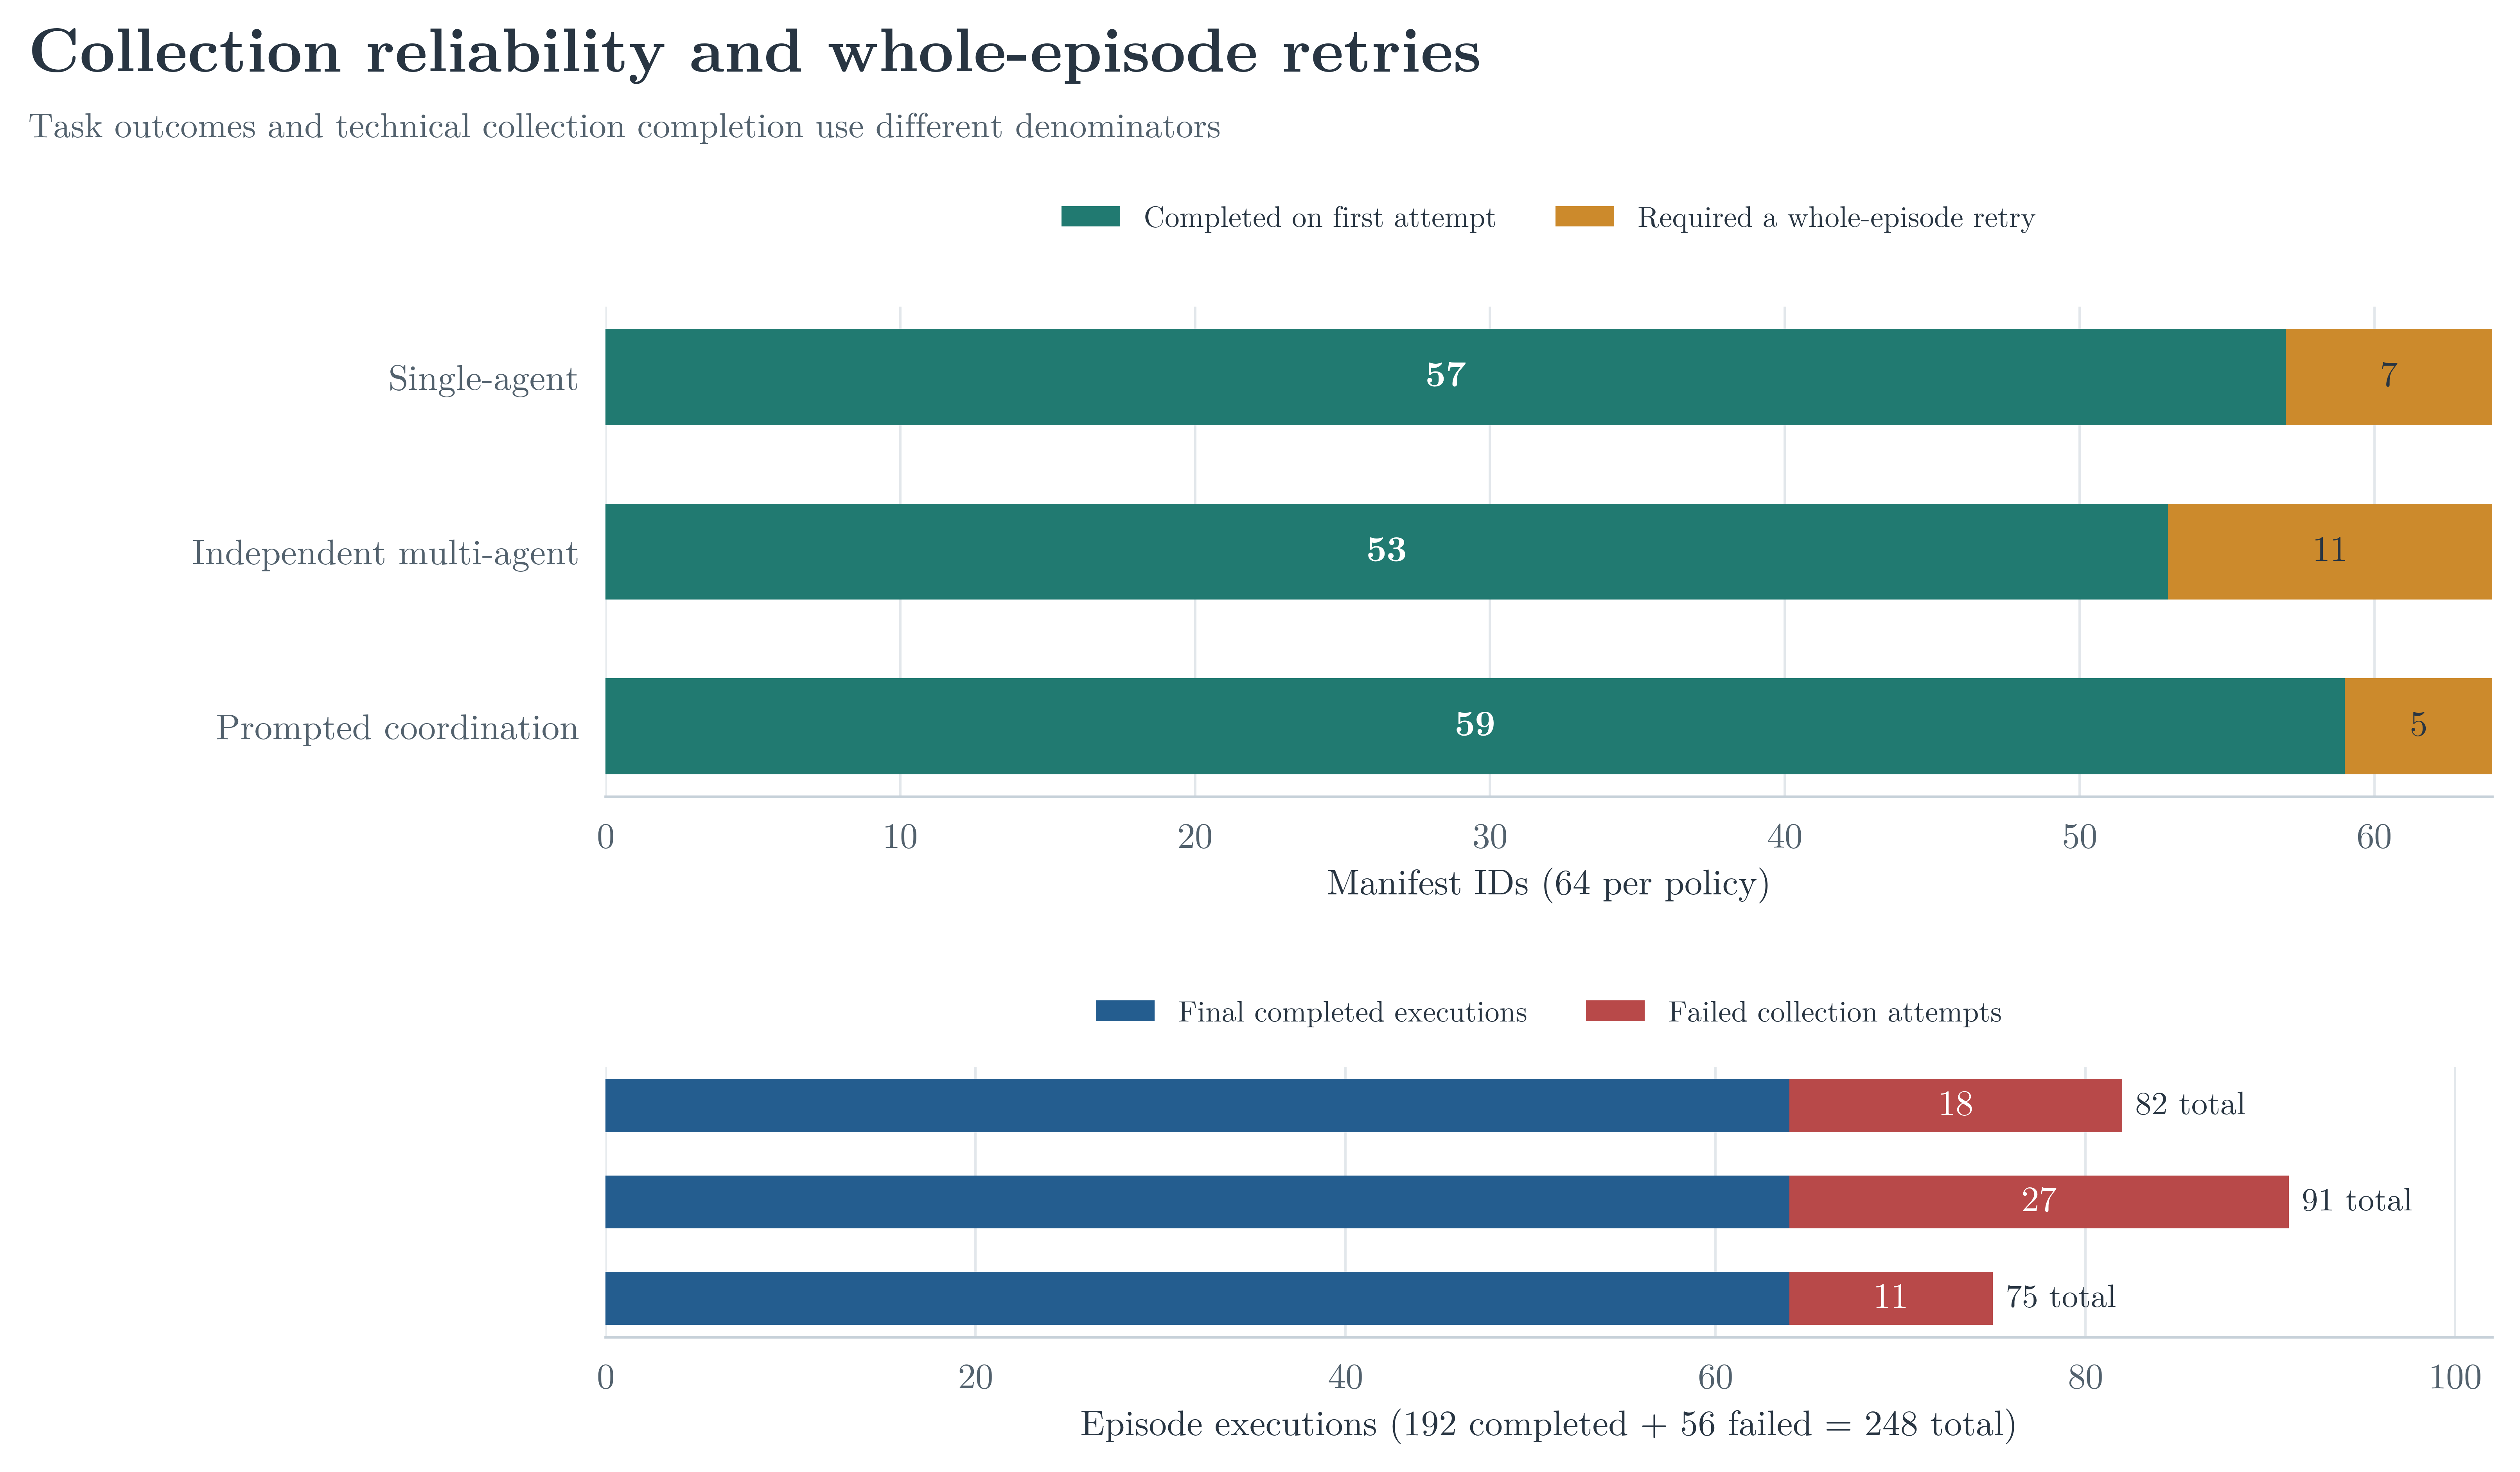
\includegraphics[width=\textwidth,height=0.68\textheight,keepaspectratio]{Images/13_retry_burden.png}
\caption{Recoverable invalid responses in final episodes and failed whole-episode collection attempts are separate mechanisms and are not interchangeable counts.}
\label{figure:14}
\end{figure}
\section{Categorical coordination analysis}
The saved \texttt{coordination\allowbreak\_report.json} reports exploratory plug-in categorical mutual information between a joint pair of agent action profiles and the episode outcome, \$I((A\allowbreak\_0,A\allowbreak\_1);Y)\$, in bits. Each agent’s profile is derived from action-abstraction counts capped at two, then reduced to one of six categories: \texttt{no\allowbreak\_actions}, \texttt{retrieved}, \texttt{verified}, \texttt{updated}, \texttt{finalized}, or \texttt{error\allowbreak\_or\allowbreak\_noop}. The encoder prioritizes error/no-op, finalization, update, verification, then retrieval, so it deliberately discards order and many distinctions in action counts. See Section 5.7 for a worked example of how \texttt{finalized} masks prior actions (\texttt{coordination\allowbreak\_analysis.py}; \texttt{coordination\allowbreak\_metrics.py}).

\begin{table}[htbp]
\centering
\fontsize{8.5}{9.5}\selectfont
\setlength{\tabcolsep}{2pt}
\renewcommand{\arraystretch}{1.2}
\begin{tabular}{|>{\raggedright\arraybackslash}p{2.4cm}|>{\centering\arraybackslash}p{1.7cm}|>{\centering\arraybackslash}p{1.6cm}|>{\centering\arraybackslash}p{1.3cm}|>{\centering\arraybackslash}p{1.6cm}|>{\centering\arraybackslash}p{1.25cm}|>{\raggedright\arraybackslash}p{2.4cm}|>{\centering\arraybackslash}p{1.7cm}|}
\hline
\shortstack[c]{\textbf{Policy}\\\textbf{condition}} & \shortstack[c]{\textbf{Eligible}\\\textbf{paired}\\\textbf{episodes}} & \shortstack[c]{\textbf{Unique}\\\textbf{joint source}\\\textbf{states}} & \shortstack[c]{\textbf{Observed}\\\textbf{outcomes}} & \shortstack[c]{\textbf{Outcome}\\\textbf{entropy}\\\textbf{(bits)}} & \shortstack[c]{\textbf{MI}\\\textbf{(bits)}} & \shortstack[c]{\textbf{95\%}\\\textbf{bootstrap}\\\textbf{interval}} & \shortstack[c]{\textbf{Permutation}\\\textbf{p-value}} \\
\hline
\shortstack[l]{Independent\\multi-agent} & 64 & 3 & 2 & 0.3373 & 0.046617 & \shortstack[c]{[0.001735,\\0.197643]} & 0.207171 \\
\hline
\shortstack[l]{Prompted\\coordination} & 58 & 4 & 2 & 0.1257 & 0.040041 & \shortstack[c]{[0.000000,\\0.125826]} & 0.386454 \\
\hline
\shortstack[l]{Single-agent} & 0 of 64 & 0 & 0 & \shortstack[c]{Not\\applicable} & \shortstack[c]{Not\\estimated} & \shortstack[c]{Not\\estimated} & \shortstack[c]{Not\\estimated} \\
\hline
\end{tabular}
\caption{Categorical action-profile mutual-information estimates}
\end{table}
Outcome entropy is empirical Shannon entropy of the outcome labels in each MI-eligible sample: it contextualizes the available variation, with lower entropy here reflecting the small partial-outcome counts. The single-agent arm has no eligible two-agent MI sample; its separate one-agent reference has only successes and therefore zero outcome entropy.

\begin{figure}[htbp]
\centering
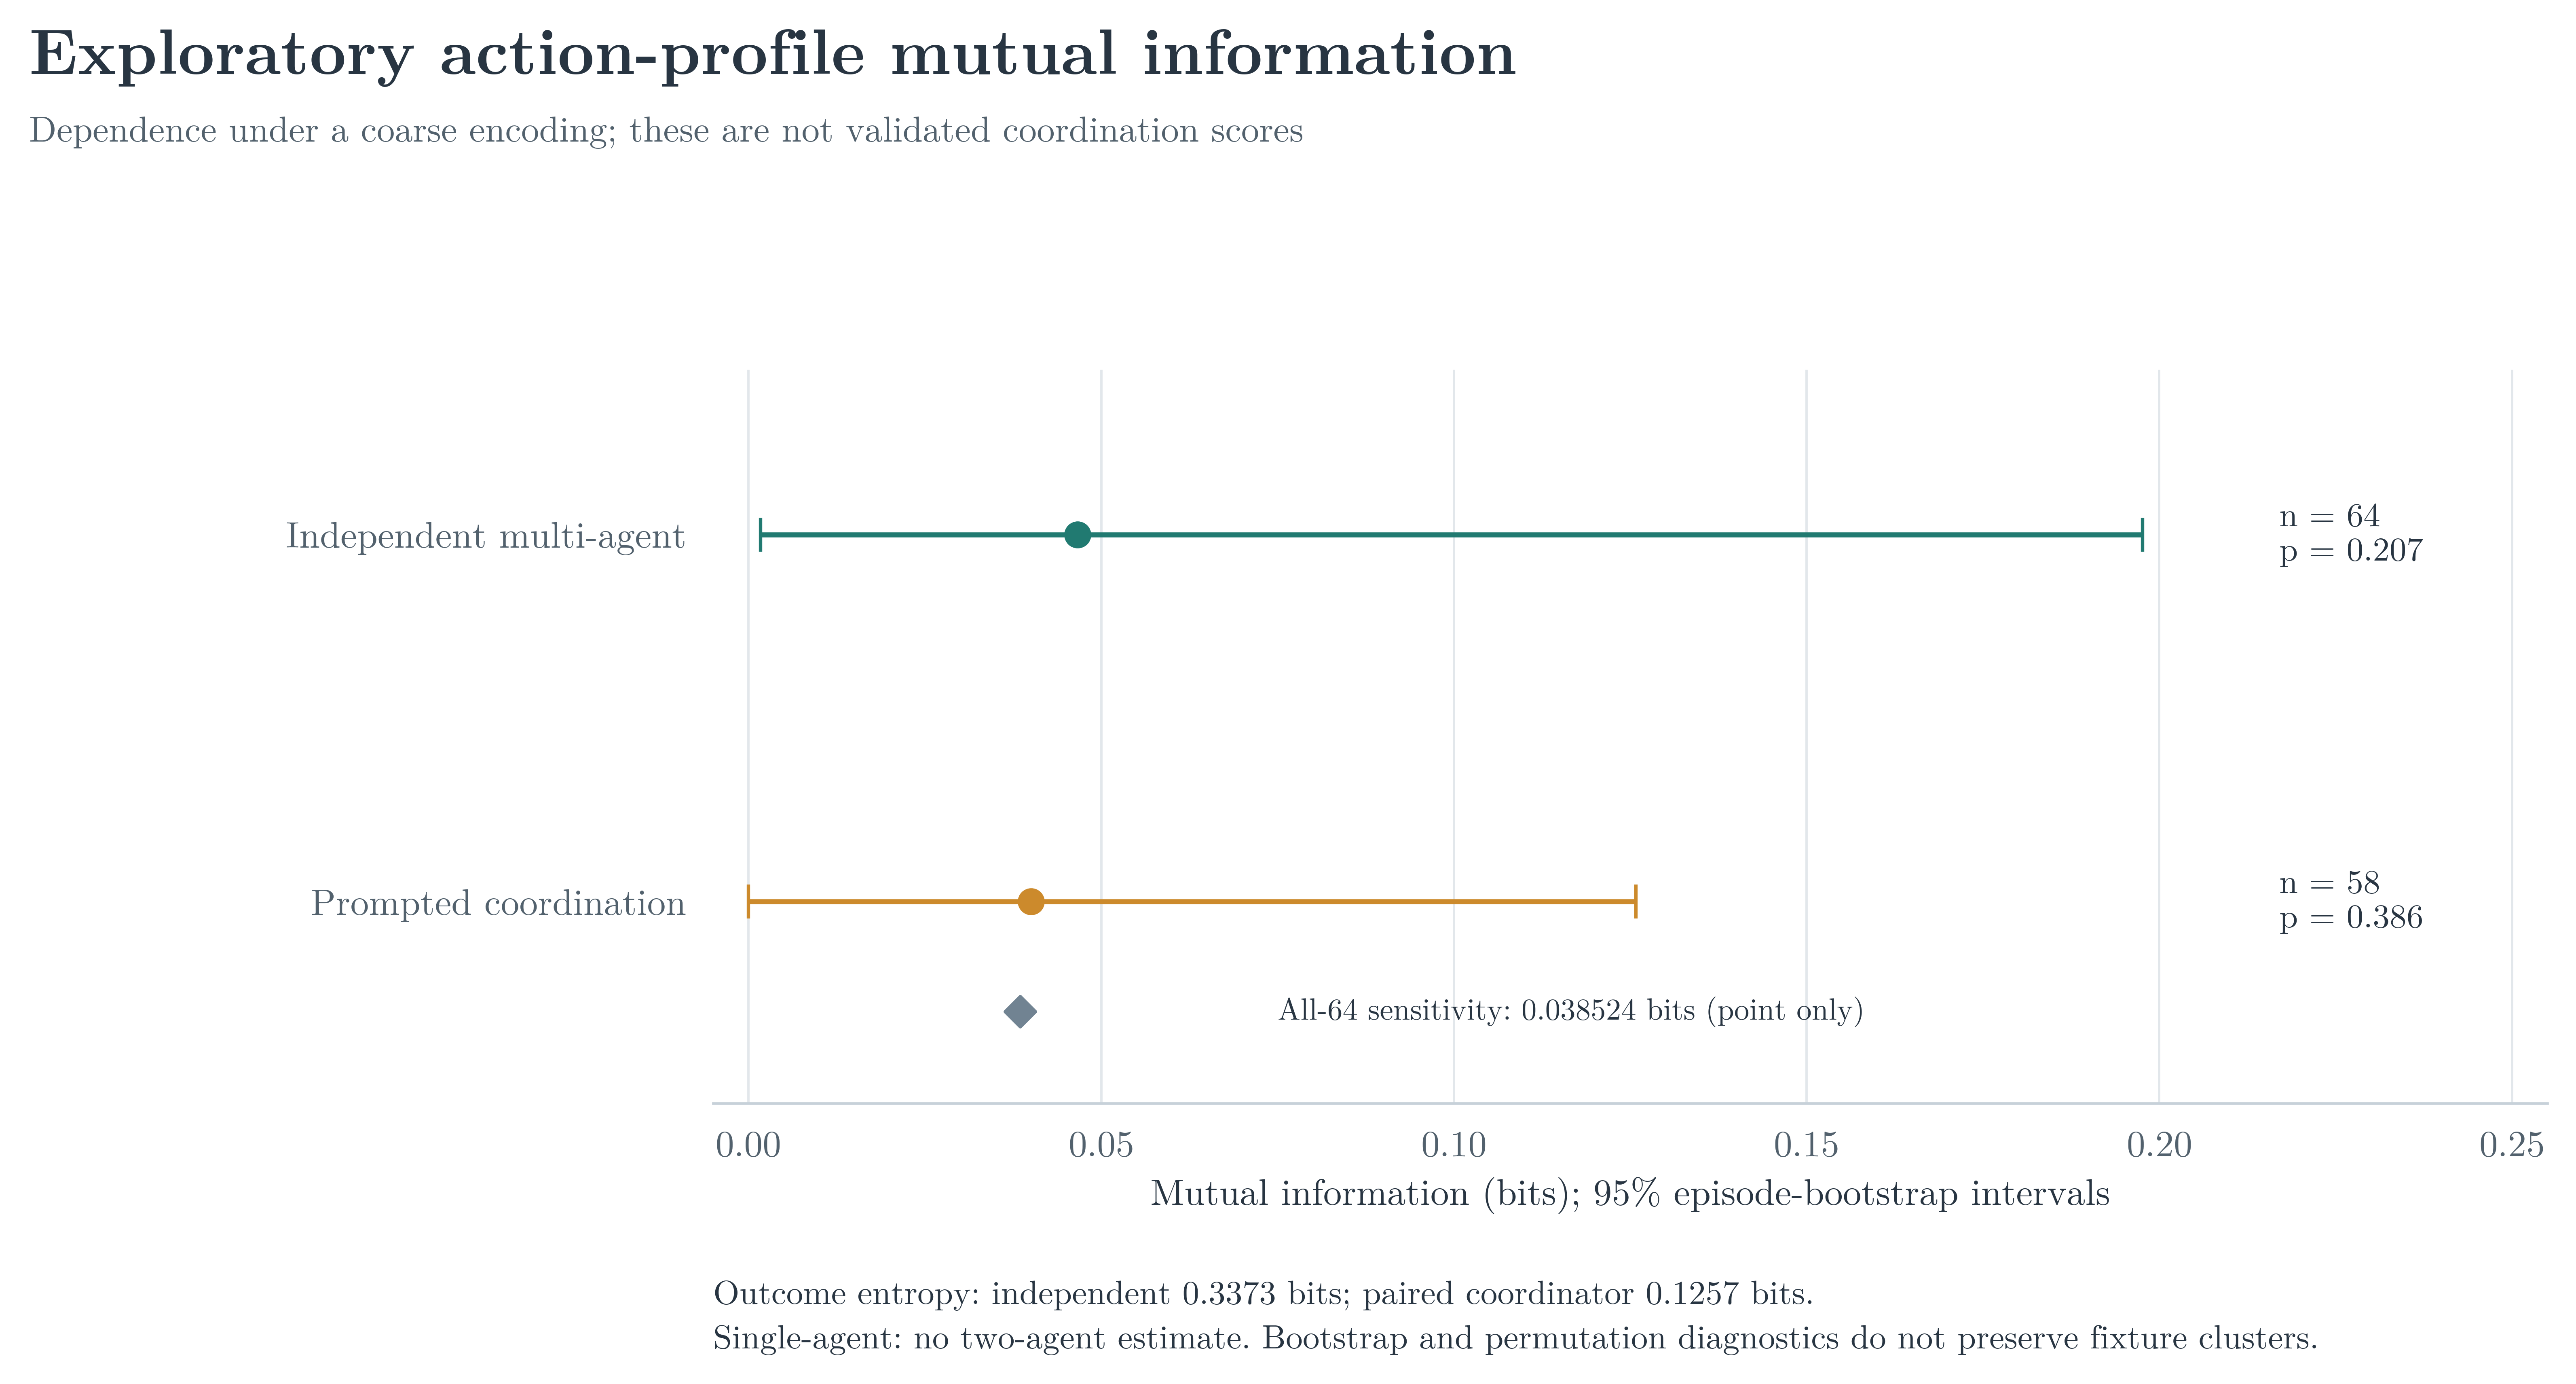
\includegraphics[width=\textwidth,height=0.68\textheight,keepaspectratio]{Images/14_mutual_information.png}
\caption{The saved plug-in categorical MI estimates and reported uncertainty diagnostics. These are exploratory associations for compressed profiles, not a validated coordination metric or a causal test.}
\label{figure:15}
\end{figure}
The following frequency tables show the exact joint-profile/outcome cells used by the two-agent plug-in MI estimates. Counts are episodes; zero cells are omitted. They make clear that this is not an inference over rich trajectories: each row is a priority-compressed joint profile, and every observed outcome is either success or partial.

\textbf{Independent multi-agent (64 episodes):}

\begin{table}[htbp]
\centering
\small
\setlength{\tabcolsep}{4pt}
\begin{tabularx}{\linewidth}{|Y|Y|Y|Y|Y|}
\hline
\textbf{Agent 0 profile} & \textbf{Agent 1 profile} & \textbf{Success} & \textbf{Partial} & \textbf{Total} \\
\hline
\texttt{finalized} & \texttt{updated} & 22 & 2 & 24 \\
\hline
\texttt{finalized} & \texttt{verified} & 1 & 1 & 2 \\
\hline
\texttt{updated} & \texttt{finalized} & 37 & 1 & 38 \\
\hline
\textbf{Total} &  & \textbf{60} & \textbf{4} & \textbf{64} \\
\hline
\end{tabularx}
\caption{Independent multi-agent action profiles by outcome}
\end{table}
\textbf{Prompted coordination, primary paired sample (58 episodes):}

\begin{table}[htbp]
\centering
\small
\setlength{\tabcolsep}{4pt}
\begin{tabularx}{\linewidth}{|Y|Y|Y|Y|Y|}
\hline
\textbf{Agent 0 profile} & \textbf{Agent 1 profile} & \textbf{Success} & \textbf{Partial} & \textbf{Total} \\
\hline
\texttt{finalized} & \texttt{retrieved} & 3 & 0 & 3 \\
\hline
\texttt{finalized} & \texttt{updated} & 11 & 1 & 12 \\
\hline
\texttt{finalized} & \texttt{verified} & 6 & 0 & 6 \\
\hline
\texttt{updated} & \texttt{finalized} & 37 & 0 & 37 \\
\hline
\textbf{Total} &  & \textbf{57} & \textbf{1} & \textbf{58} \\
\hline
\end{tabularx}
\caption{Prompted-coordination action profiles by outcome}
\end{table}
The independent-policy table has partial outcomes in all three observed joint-profile cells, with counts of two, one, and one: \texttt{finalized}/\texttt{updated}, \texttt{finalized}/\texttt{verified}, and \texttt{updated}/\texttt{finalized}, respectively. The coordinator paired table has one partial, in the \texttt{finalized}/\texttt{updated} cell. Thus the reported MI values are driven by the distribution of those few profile/outcome counts, not by broad outcome variation or a direct measure of coordination. In both tables every joint profile contains \texttt{finalized}: as all episodes end with finalization, the categorical source primarily records which actor ID received the terminal action and, for the other agent, its highest-priority remaining category. It does not preserve whether the finalizing agent also retrieved, patched, or verified earlier in the episode. This is a stopping/actor-assignment encoding as much as an action-use encoding.

The coordinator’s primary analysis excludes six episodes because only one of the two nominal agents has any recorded tool event: five have agent 0 events only and one has agent 1 events only. This is eligibility by observed event participation, not by model-response retries. The unobserved actor did not contribute an event; \texttt{no\allowbreak\_actions} does not establish what that actor privately considered or whether the coordinating policy made a meaningful decision on its behalf.

\begin{figure}[htbp]
\centering
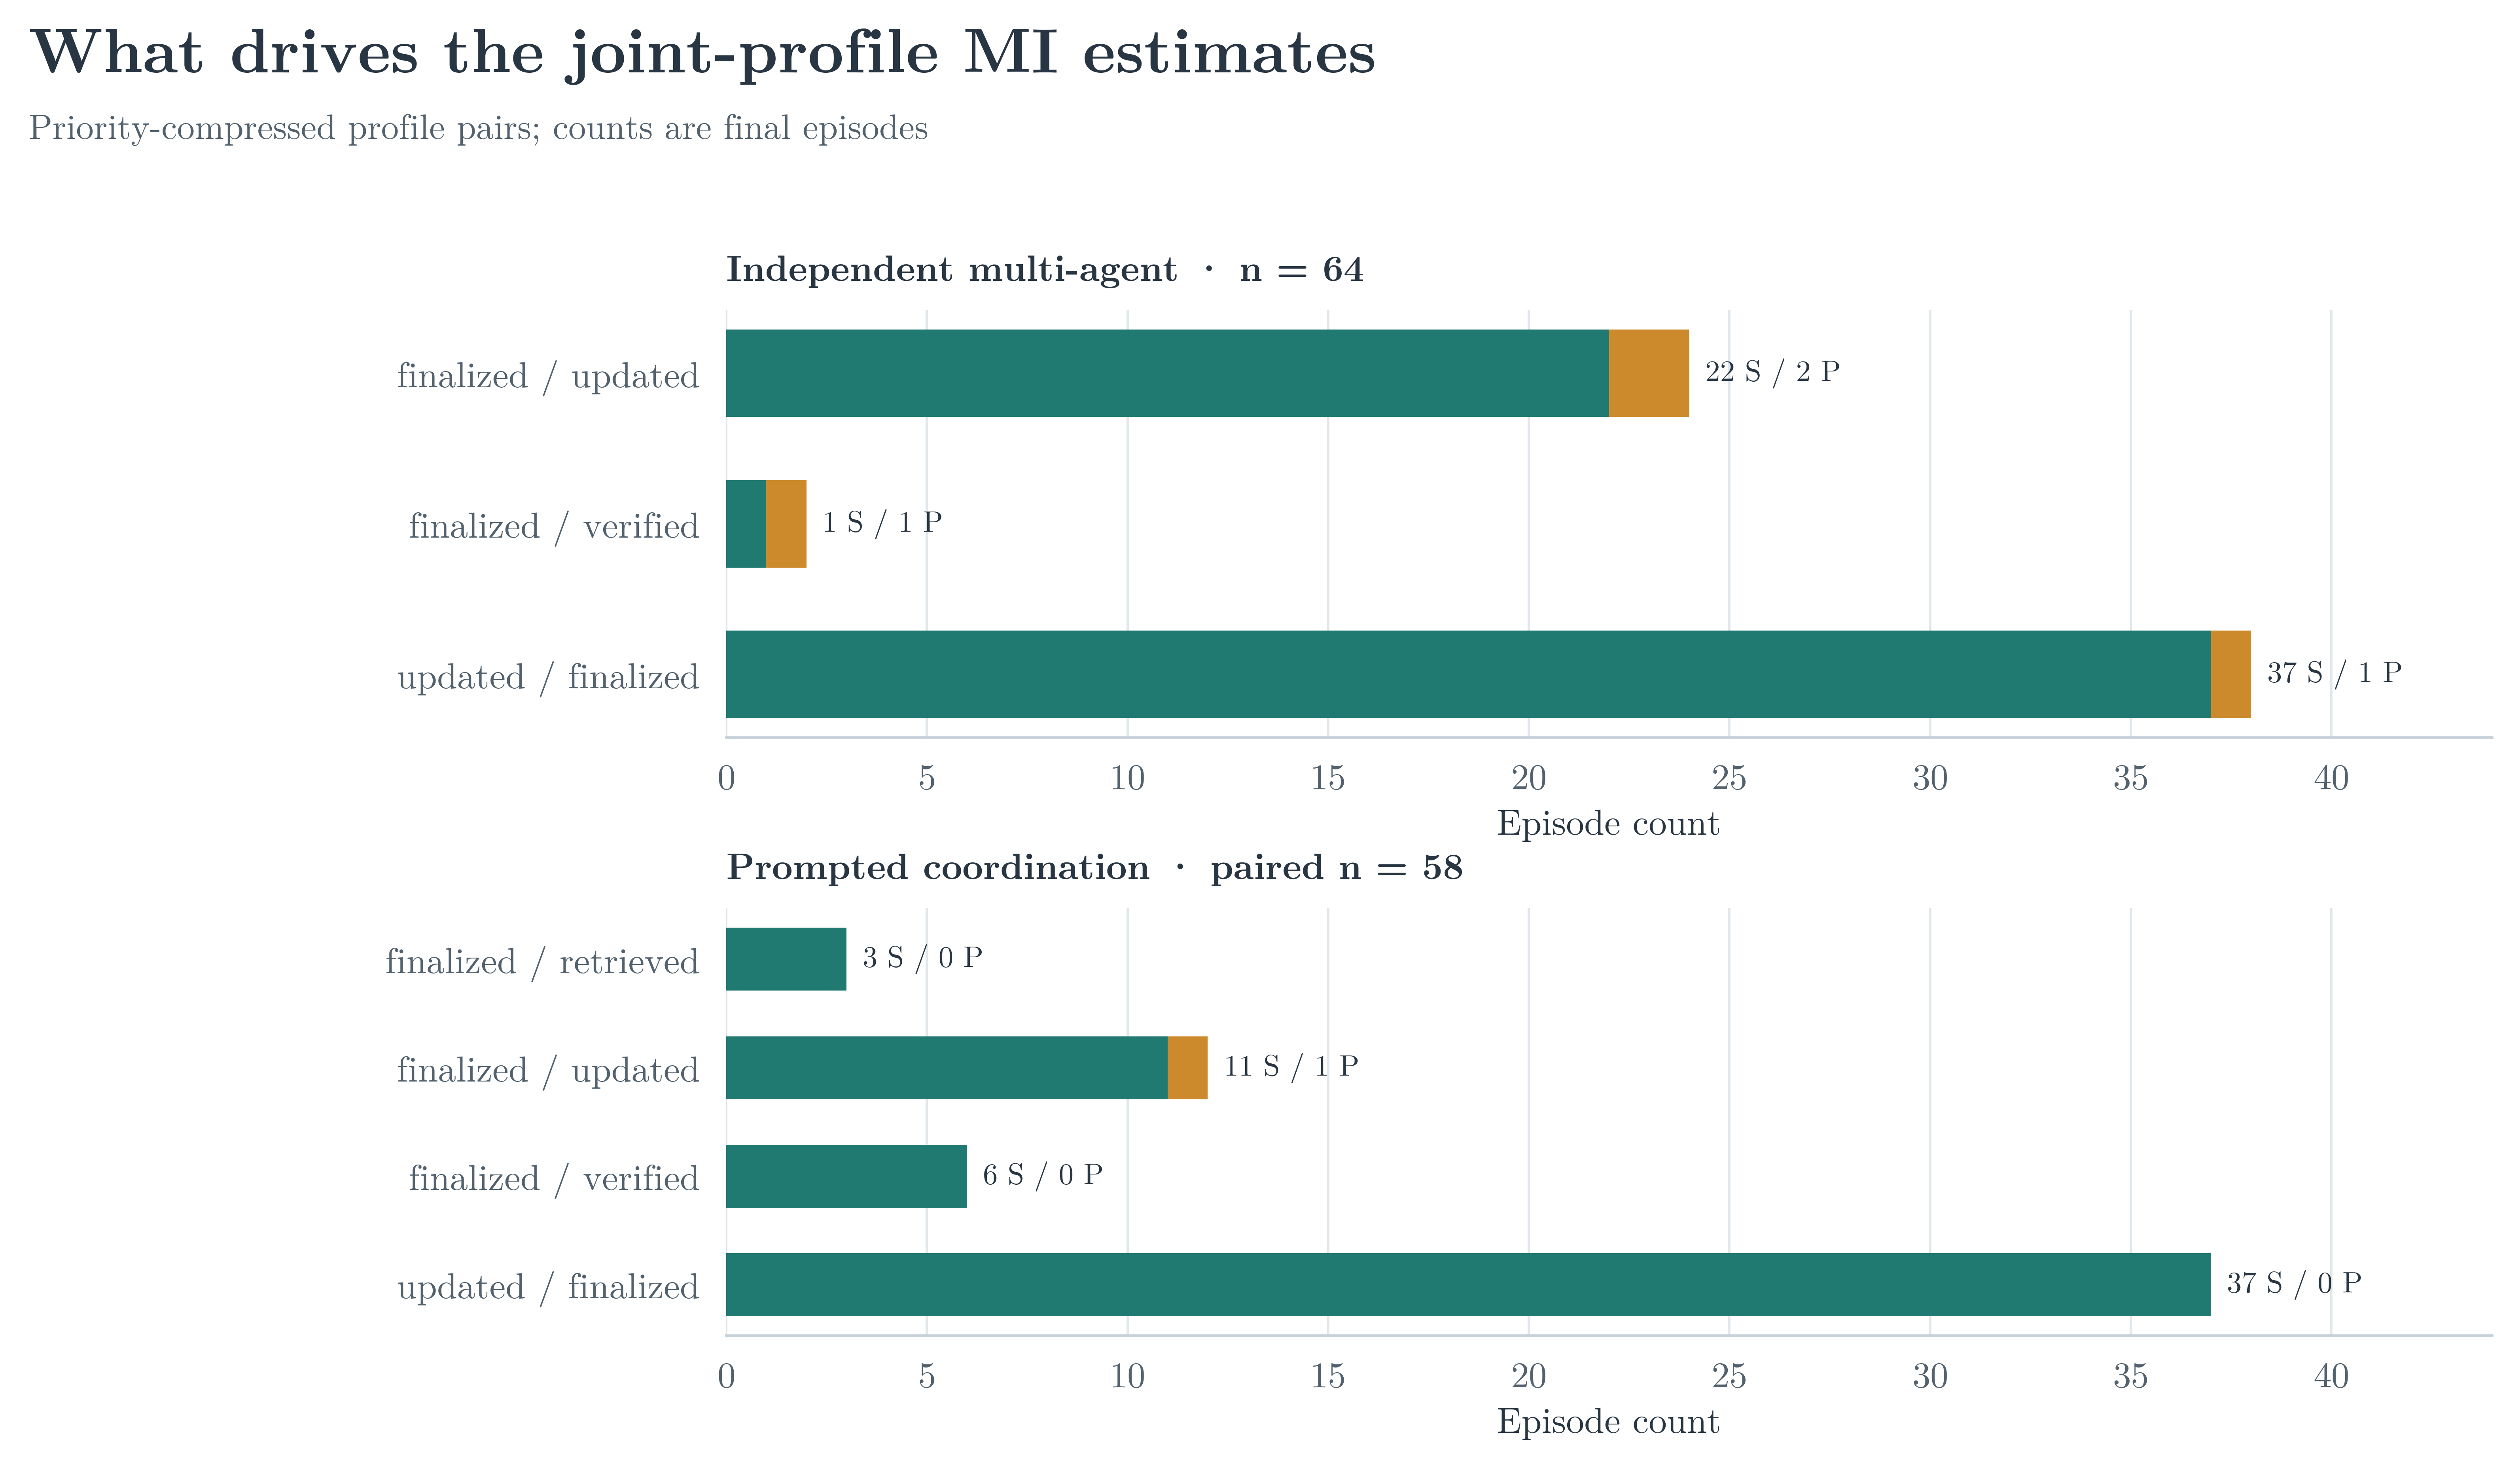
\includegraphics[width=\textwidth,height=0.68\textheight,keepaspectratio]{Images/15_joint_profile_counts.png}
\caption{Joint action-profile/outcome counts for the independent and eligible prompted-coordination samples. Each profile contains a finalization category, reflecting the priority rule and terminal actor assignment.}
\label{figure:16}
\end{figure}
\textbf{Sensitivity: retain all 64 prompted-coordination episodes.} For this re-tabulation only, \texttt{no\allowbreak\_actions} was assigned to the nominal agent with no event in each of the six single-active episodes. All six episodes are successes. The resulting joint-profile/outcome frequencies are:

\begin{table}[htbp]
\centering
\small
\setlength{\tabcolsep}{4pt}
\begin{tabularx}{\linewidth}{|Y|Y|Y|Y|Y|}
\hline
\textbf{Agent 0 profile} & \textbf{Agent 1 profile} & \textbf{Success} & \textbf{Partial} & \textbf{Total} \\
\hline
\texttt{finalized} & \texttt{no\allowbreak\_actions} & 5 & 0 & 5 \\
\hline
\texttt{finalized} & \texttt{retrieved} & 3 & 0 & 3 \\
\hline
\texttt{finalized} & \texttt{updated} & 11 & 1 & 12 \\
\hline
\texttt{finalized} & \texttt{verified} & 6 & 0 & 6 \\
\hline
\texttt{no\allowbreak\_actions} & \texttt{finalized} & 1 & 0 & 1 \\
\hline
\texttt{updated} & \texttt{finalized} & 37 & 0 & 37 \\
\hline
\textbf{Total} &  & \textbf{63} & \textbf{1} & \textbf{64} \\
\hline
\end{tabularx}
\caption{Action profiles and outcomes by fixture family}
\end{table}
Using the same unsmoothed plug-in formula, this all-64 sensitivity estimate is \$0.038524\$ bits, compared with \$0.040041\$ bits on the 58 paired episodes. Retaining the six episodes therefore lowers the point estimate slightly; it does not change the substantive interpretation. It also adds two profile states that mark the inactive event actor, which can themselves be predictive because all six corresponding outcomes are successes. This is a retrospective sensitivity analysis; \texttt{no\allowbreak\_actions} is an event-trace absence label, not a validated measure of agent inactivity.

\textbf{Fixture-family composition.} Every fixture family contributes eight episodes per two-agent policy. The table gives the number of episodes in each family with joint profiles \texttt{finalized/updated} (F/U), \texttt{updated/finalized} (U/F), and all other observed pairs; partials are listed separately. It shows that profiles vary with fixture family, while all partial outcomes are confined to billing.

\begin{table}[htbp]
\centering
\fontsize{8.5}{9.5}\selectfont
\setlength{\tabcolsep}{2pt}
\renewcommand{\arraystretch}{1.15}
\begin{tabular}{|>{\raggedright\arraybackslash}p{2.4cm}|>{\centering\arraybackslash}p{1.45cm}|>{\centering\arraybackslash}p{1.45cm}|>{\centering\arraybackslash}p{1.45cm}|>{\centering\arraybackslash}p{1.45cm}|>{\centering\arraybackslash}p{1.45cm}|>{\centering\arraybackslash}p{1.45cm}|>{\centering\arraybackslash}p{1.45cm}|>{\centering\arraybackslash}p{1.45cm}|}
\hline
\shortstack[c]{\textbf{Fixture}\\\textbf{family}} & \shortstack[c]{\textbf{Indep.}\\\textbf{F/U}} & \shortstack[c]{\textbf{Indep.}\\\textbf{U/F}} & \shortstack[c]{\textbf{Indep.}\\\textbf{other}} & \shortstack[c]{\textbf{Indep.}\\\textbf{partial}} & \shortstack[c]{\textbf{Coord.}\\\textbf{F/U}} & \shortstack[c]{\textbf{Coord.}\\\textbf{U/F}} & \shortstack[c]{\textbf{Coord.}\\\textbf{other}} & \shortstack[c]{\textbf{Coord.}\\\textbf{partial}} \\
\hline
\texttt{billing} & 4 & 2 & 2 & 4 & 2 & 4 & 2 & 1 \\
\hline
\texttt{flag\allowbreak\_parser} & 2 & 6 & 0 & 0 & 3 & 3 & 2 & 0 \\
\hline
\texttt{inventory} & 2 & 6 & 0 & 0 & 3 & 2 & 3 & 0 \\
\hline
\texttt{math\allowbreak\_ops} & 3 & 5 & 0 & 0 & 1 & 6 & 1 & 0 \\
\hline
\texttt{ranking} & 3 & 5 & 0 & 0 & 1 & 4 & 3 & 0 \\
\hline
\texttt{retry\allowbreak\_policy} & 3 & 5 & 0 & 0 & 1 & 6 & 1 & 0 \\
\hline
\texttt{scheduler} & 2 & 6 & 0 & 0 & 0 & 6 & 2 & 0 \\
\hline
\texttt{string\allowbreak\_utils} & 5 & 3 & 0 & 0 & 1 & 6 & 1 & 0 \\
\hline
\textbf{Total} & \textbf{24} & \textbf{38} & \textbf{2} & \textbf{4} & \textbf{12} & \textbf{37} & \textbf{15} & \textbf{1} \\
\hline
\end{tabular}
\caption{Fixture-family outcomes and action categories}
\end{table}
Here “other” includes \texttt{finalized/verified}, \texttt{finalized/retrieved}, and (for the all-64 coordinator table) pairs containing \texttt{no\allowbreak\_actions}. Existing fixture-outcome counts show 19/24 billing successes and 168/168 successes in the other families (Section 9.5.1). Thus task family/difficulty is a plausible common cause of both action-profile distribution and outcome: billing both differs in profile composition and contains all observed partials. The remaining families’ profile mixtures also differ despite all-success outcomes, but the design and cell sizes do not disentangle policy behavior from fixture effects. The pooled MI is not adjusted or stratified by fixture; it cannot tell whether profile/outcome dependence reflects coordination, fixture difficulty, or their combination. Fixture-matched assignment across policies improves coverage comparability but does not remove this within-condition confounding.

The percentile intervals were computed from 500 ordinary episode-level bootstrap resamples. The permutation null shuffled outcome labels relative to action profiles over 250 iterations, with a plus-one correction; the observed p-values are 0.207171 and 0.386454. For the independent policy, the bootstrap interval's lower endpoint is above zero while the permutation result is nonsignificant because the procedures answer different questions. The bootstrap resamples the observed joint-profile/outcome pairs to describe sampling variability around the empirical plug-in estimate; it does not impose a no-association null. The plug-in MI estimate is nonnegative, and its finite-sample value can be upward biased. In this run, the 2.5th percentile of the resampled empirical estimates remained above zero, so the percentile interval excluded zero. The permutation procedure instead breaks the observed pairing of profile and outcome by shuffling outcome labels, approximating a null distribution for no association while retaining the observed marginal label counts. A p-value of 0.207 does not provide evidence against that null at conventional thresholds. Thus, a percentile interval for a nonnegative plug-in estimate is not a null test, and the two results are not contradictory. The ordinary episode bootstrap and unrestricted outcome shuffle also do not preserve fixture clusters, so these MI diagnostics are exploratory and do not adjust for repeated fixtures.

Rebuilding the paired datasets from all saved \texttt{episode.jsonl} files reproduces the sample sizes, unique states/outcomes, and MI point estimates. Re-running the saved analysis over those files also reproduces both intervals and p-values exactly. The independent-policy smoothing sensitivity is 0.046617, 0.052821, and 0.056560 bits at alpha 0, 0.5, and 1.0; the corresponding paired-coordinator values are 0.040041, 0.032397, and 0.039309 bits. The all-64 coordinator sensitivity above is an additional unsmoothed point estimate only; no interval or permutation test was computed for it. These diagnostics remain exploratory and are another reminder that the values are estimates over a small number of observed categories, not invariant behavioral quantities.

The MI values are small and the observed paired action-profile support is limited to three or four joint states. Outcome entropy is only 0.3373 bits for independent multi-agent and 0.1257 bits for the paired coordinator subset, compared with a maximum of one bit for a balanced binary outcome. The full-64 coordinator sensitivity has six joint profile states, a single partial, and outcome entropy of 0.1161 bits. These low entropies make clear that the outcomes available to explain are highly restricted. The estimates summarize empirical dependence for the encoded categories; they do not establish that an action pattern caused a successful outcome or that one policy is more coordinated than another. The bootstrap and permutation outputs are diagnostics for each condition’s own categorical association. They are not a test comparing the two policies’ MI values or success rates. In light of the terminal-action priority rule, fixture-family composition, and six event-inactive coordinator episodes, MI remains exploratory rather than evidence of coordination.

The single-agent condition is not a two-agent comparison: its episodes contain one agent’s trace, so no joint source \$(A\allowbreak\_0,A\allowbreak\_1)\$ exists. All 64 episodes are therefore ineligible for two-agent MI. A separate one-agent reference contains 64 episodes, one unique encoded action-profile state, all-success outcomes, and MI of zero. That reference is structurally different and has no outcome variation; it cannot be placed on the same footing as the two-agent estimates or used to infer the effect of adding an agent.

Finally, this categorical statistic is not the paper’s time-delayed mutual information or partial information decomposition. It does not estimate predictive synergy, redundancy, differentiation, or complementarity. The action profile is an intentionally coarse representation to keep observed state cardinality manageable, and its labels do not validate the semantic importance of an agent’s contribution.

\section{Retrospective agent participation and fixture-level outcomes}
To supplement the outcome-linked categorical MI analysis, the final run's 192 saved episode summaries and 1,181 \texttt{episode.jsonl} tool events were reanalyzed without making new model calls. This follow-up uses the same completed episodes reported in Section 9.2; it is not an additional experimental sample. The two-agent conditions each contribute 64 episodes to the workload analysis, while all three conditions contribute to the fixture-level outcome analysis. Counts were reconciled against the final-run aggregate and manifest (manifest). Interpretation of the independent-versus-prompted contrast is constrained by a bundled policy change: the coordinator condition changes both role instructions and actor-selection authority, as detailed in Section 5.3. In particular, workload differences cannot be interpreted as an effect of coordination prompting alone.

\textbf{Agent participation.} For each two-agent episode, valid recorded tool events were counted by \texttt{agent\allowbreak\_id}, and normalized workload imbalance was calculated as \$|n\allowbreak\_0-n\allowbreak\_1|/(n\allowbreak\_0+n\allowbreak\_1)\$, where \$n\allowbreak\_i\$ is the tool-call count of agent \$i\$. The table reports the unweighted mean across all 64 episodes in each condition. Tool-mix total variation distance (TVD), \$\textbackslash\{\}tfrac\{1\}\{2\}\textbackslash\{\}sum\allowbreak\_t |p\allowbreak\_0(t)-p\allowbreak\_1(t)|\$, was also calculated to compare each agent's proportions across the five tool types. TVD is defined only when \emph{both} agents acted, so its denominator differs for the two policies.

\begin{table}[htbp]
\centering
\small
\setlength{\tabcolsep}{4pt}
\begin{tabularx}{\linewidth}{|Y|Y|Y|Y|Y|Y|}
\hline
\textbf{Two-agent condition} & \textbf{Agent 0 calls} & \textbf{Agent 1 calls} & \textbf{Mean workload imbalance} & \textbf{Only one agent active} & \textbf{Mean tool-mix TVD (both active)} \\
\hline
\texttt{llm\allowbreak\_independent\allowbreak\_multi\allowbreak\_agent} & 210 & 184 & 6.81\% & 0/64 & 0.480 (64 episodes) \\
\hline
\texttt{llm\allowbreak\_prompted\allowbreak\_coordination} & 228 & 143 & 33.08\% & 6/64 & 0.884 (58 episodes) \\
\hline
\end{tabularx}
\caption{Participation and workload by agent}
\end{table}
The prompted-coordination condition exhibits more unequal participation and larger differences in the \emph{types} of tools used by its two active agents. In that condition, agent 0 performed 109 \texttt{apply\allowbreak\_patch} calls versus 26 by agent 1, whereas agent 1 performed 64 \texttt{run\allowbreak\_tests} calls versus 36 by agent 0. This pattern is consistent with differentiated action assignment, but it is \textbf{not evidence of emergent specialization}: the independent policy alternates preferred actors, whereas the coordinator policy may assign actions to either agent. Actor IDs are policy labels, and neither workload imbalance nor TVD establishes why particular actions were assigned or whether the division of work helped completion. The six single-active-agent episodes remain included in the imbalance mean but cannot contribute to tool-mix TVD because the inactive agent has no observed tool distribution.

\begin{figure}[htbp]
\centering
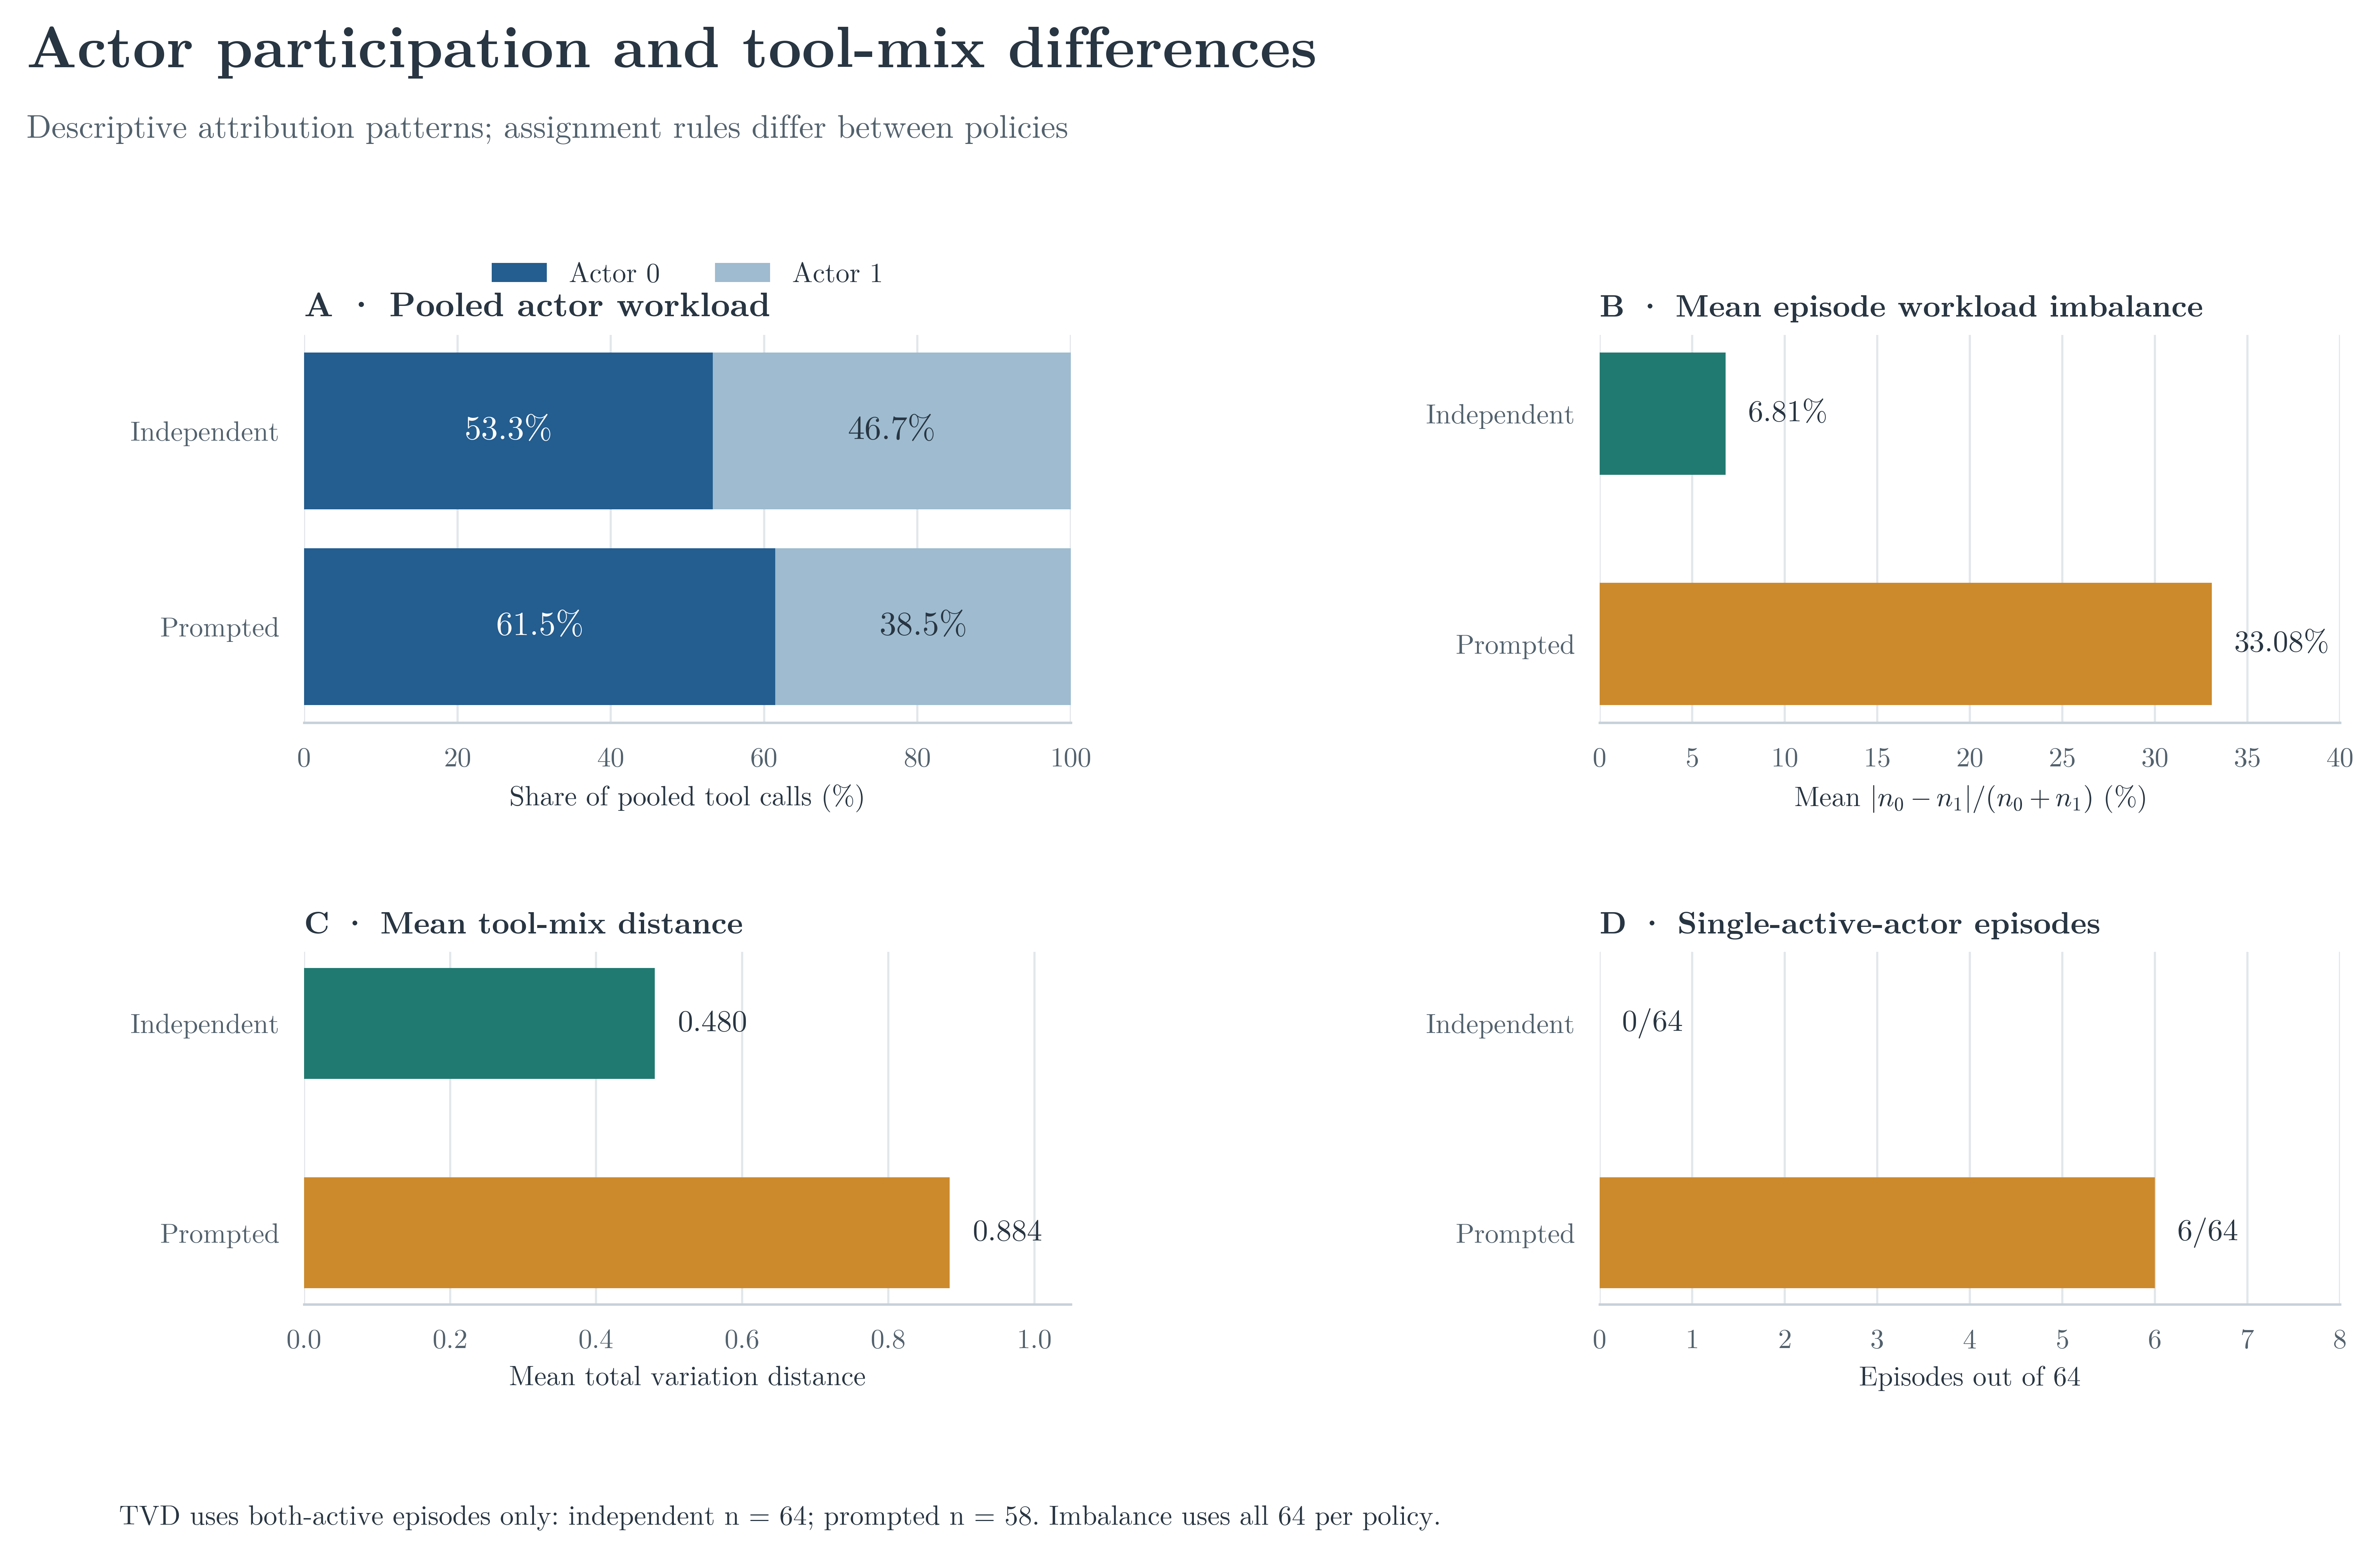
\includegraphics[width=\textwidth,height=0.68\textheight,keepaspectratio]{Images/16_actor_participation.png}
\caption{Retrospective workload and tool-mix differences by nominal actor. The actor IDs and assignment rules are policy-defined, so these differences are not evidence of emergent specialization.}
\label{figure:17}
\end{figure}
\textbf{Fixture-level outcomes.} Aggregating the same final-run summaries by fixture family reveals that every partial outcome belongs to the billing family; the other seven families have no partials or failures in this run.

\begin{table}[htbp]
\centering
\small
\setlength{\tabcolsep}{4pt}
\begin{tabularx}{\linewidth}{|Y|Y|Y|Y|Y|Y|}
\hline
\textbf{Fixture family} & \textbf{Episodes} & \textbf{Success} & \textbf{Partial} & \textbf{Failure} & \textbf{Success rate} \\
\hline
\texttt{billing} & 24 & 19 & 5 & 0 & 79.17\% \\
\hline
\texttt{flag\allowbreak\_parser} & 24 & 24 & 0 & 0 & 100.00\% \\
\hline
\texttt{inventory} & 24 & 24 & 0 & 0 & 100.00\% \\
\hline
\texttt{math\allowbreak\_ops} & 24 & 24 & 0 & 0 & 100.00\% \\
\hline
\texttt{ranking} & 24 & 24 & 0 & 0 & 100.00\% \\
\hline
\texttt{retry\allowbreak\_policy} & 24 & 24 & 0 & 0 & 100.00\% \\
\hline
\texttt{scheduler} & 24 & 24 & 0 & 0 & 100.00\% \\
\hline
\texttt{string\allowbreak\_utils} & 24 & 24 & 0 & 0 & 100.00\% \\
\hline
\textbf{Total} & \textbf{192} & \textbf{187} & \textbf{5} & \textbf{0} & \textbf{97.40\%} \\
\hline
\end{tabularx}
\caption{Final outcomes by fixture family}
\end{table}
Within the billing family, the single-agent policy succeeded in 8/8 episodes (100\%), independent multi-agent in 4/8 (50\%), and prompted coordination in 7/8 (87.5\%). Each family contains two fixture variants and four repetitions per condition. As detailed in Section 9.2.1, all five billing partials finalized with a required defect unresolved and tool-call budget remaining. These results identify where the incomplete outcomes occurred and make the near-ceiling overall success rate less misleading. However, the per-condition billing samples comprise only eight episodes each, the tasks are synthetic, and these descriptive contrasts do not establish policy superiority or a causal benefit from coordination. The supplementary analysis can be reproduced from the saved final-run data.

\begin{figure}[htbp]
\centering
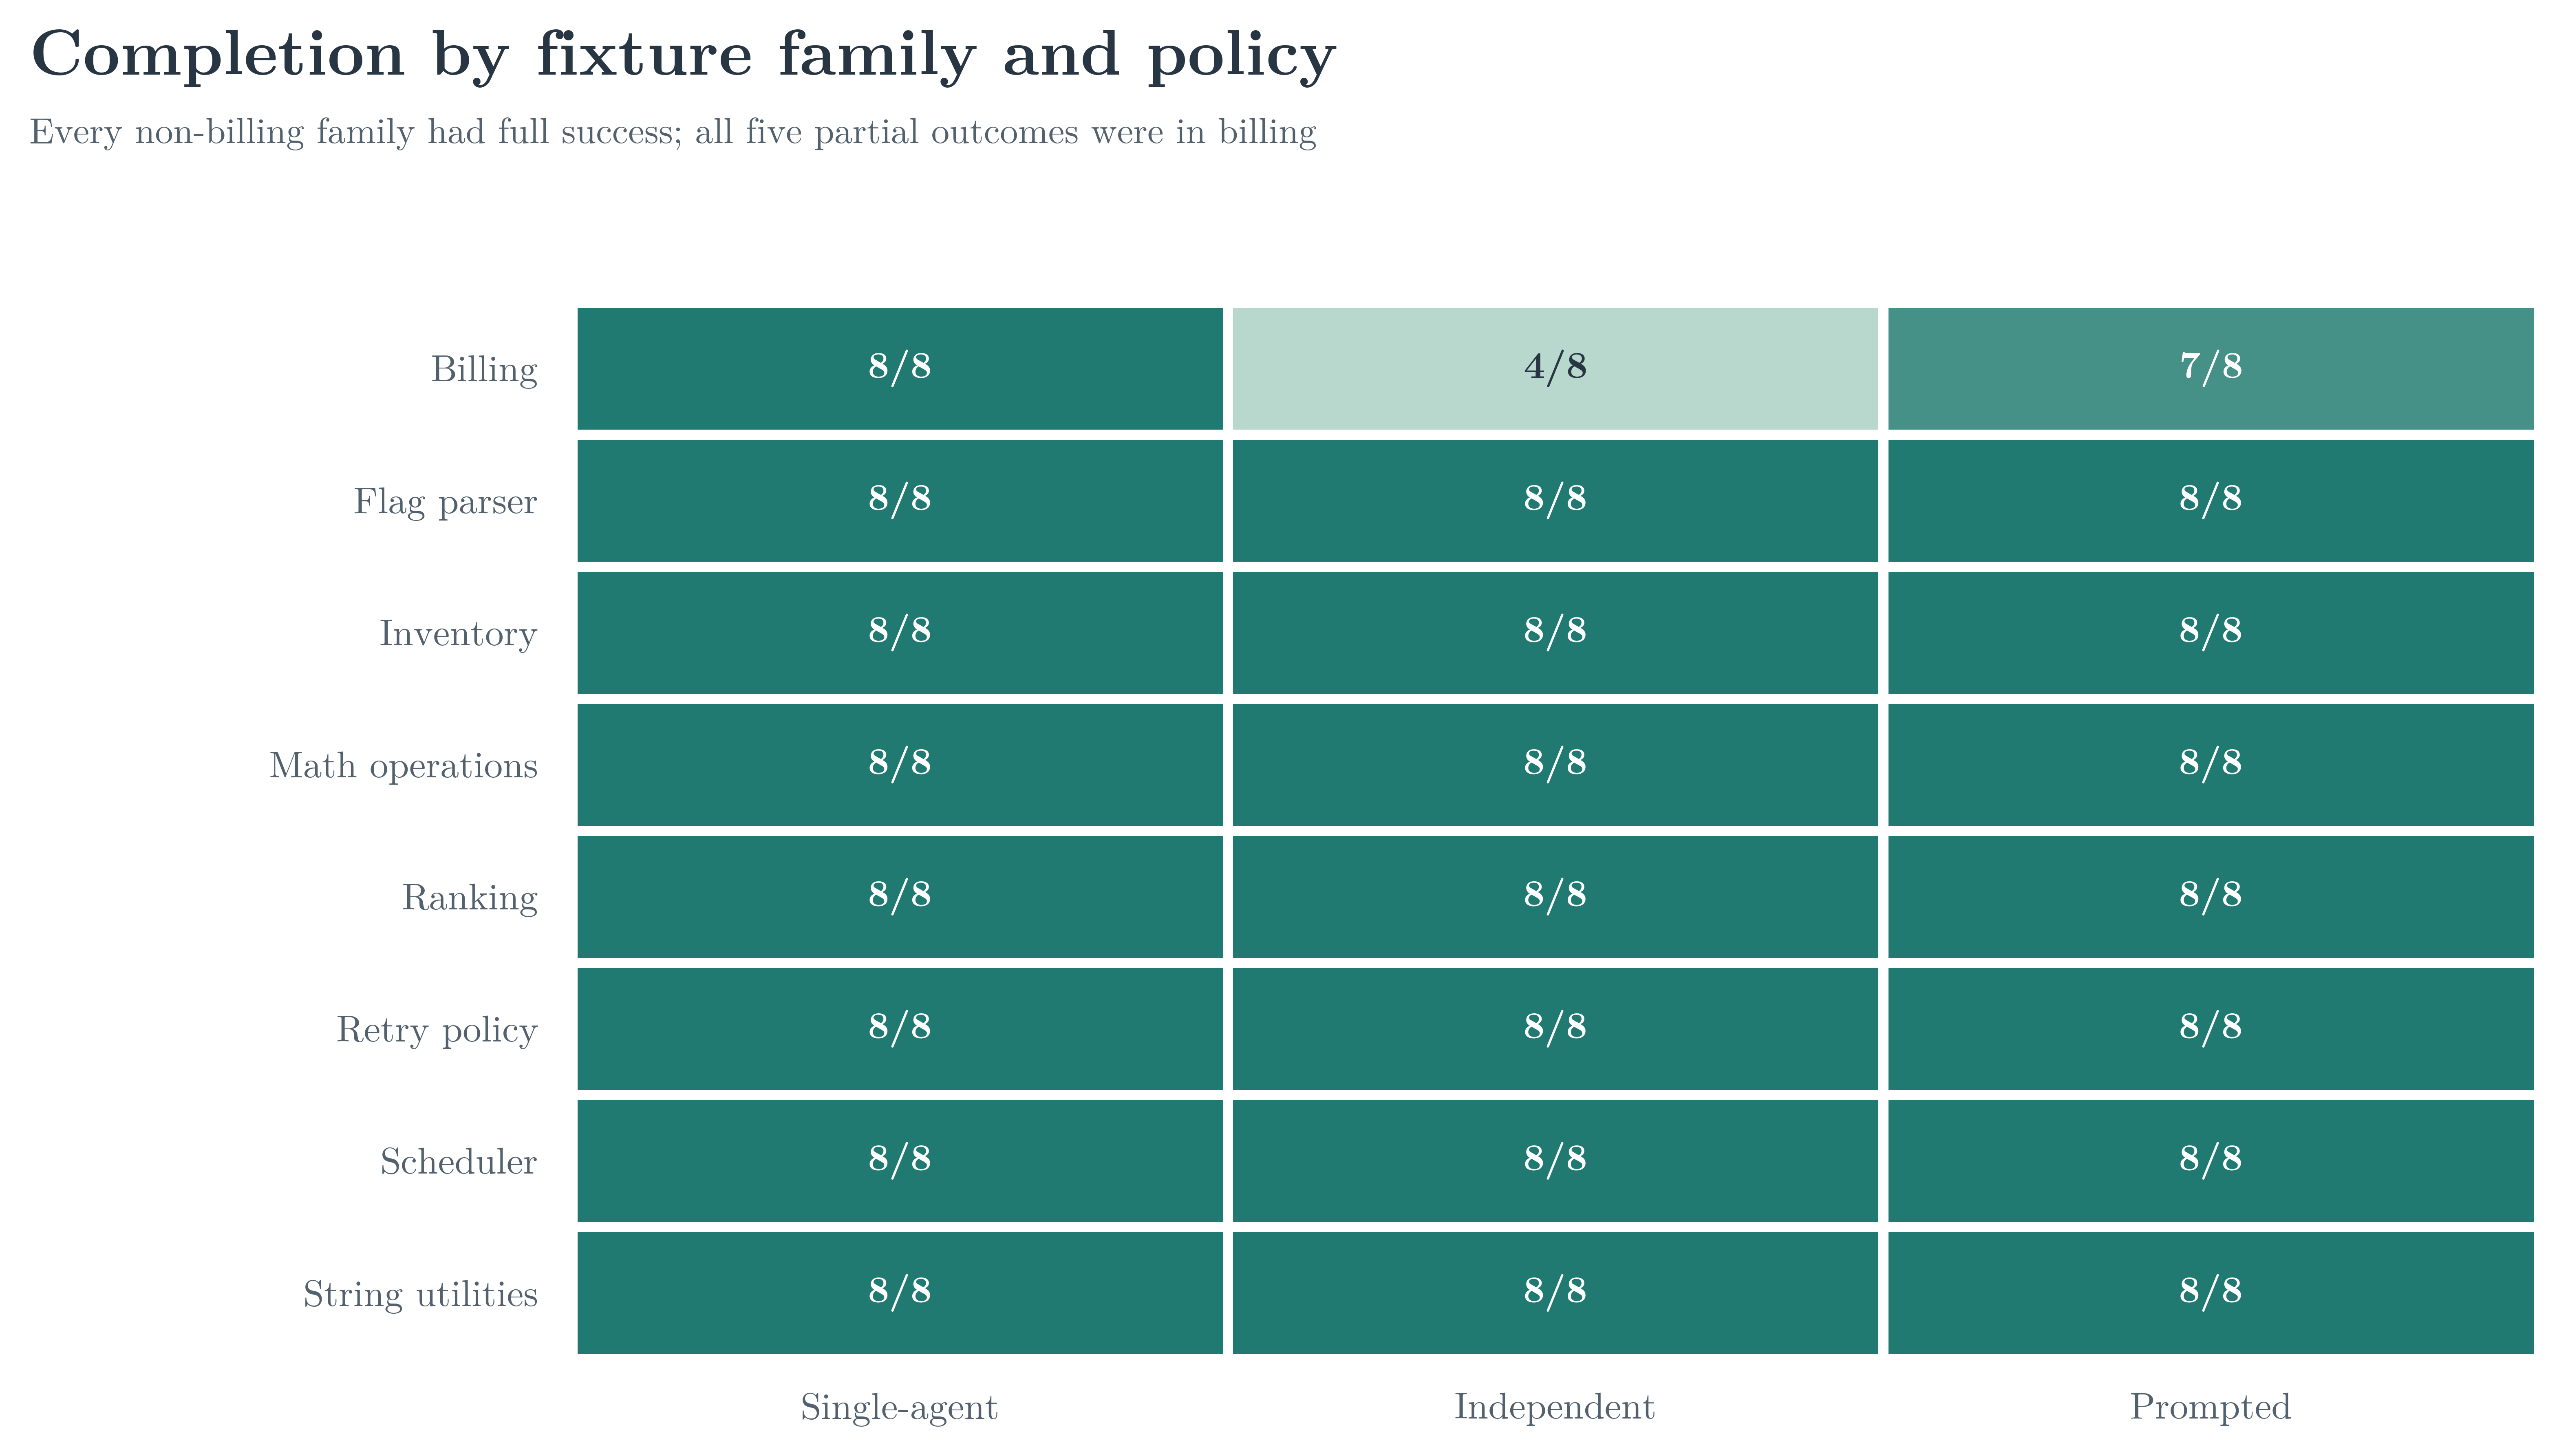
\includegraphics[width=\textwidth,height=0.68\textheight,keepaspectratio]{Images/17_fixture_family_outcomes.png}
\caption{The five partial outcomes are confined to billing in this saved run. This is a descriptive pattern in the engineered fixture set, not a general estimate of task difficulty.}
\label{figure:18}
\end{figure}
\section{Artifact integrity, exports, and limitations}
The saved \texttt{thesis\allowbreak\_results\allowbreak\_qc.md} reports passing coverage, export, ordering, hash-consistency, and strict-audit checks. In a targeted audit, the core episode-level relationships were checked: all 192 episodes have a JSONL header, summary, and task fixture; each summary’s condition, seed, fixture, and repetition matches its manifest record; fixture IDs match; event counts equal both \texttt{event\allowbreak\_count} and calls to completion; per-episode event sequence IDs are contiguous; and header/event config hashes match their summaries. No malformed episodes were returned by the saved coordination collector. All 1,181 events reconcile with summary counts. These targeted identity/count/order/hash-consistency checks do not amount to comprehensive schema, semantic, or replay validation.

The \texttt{exports/export\allowbreak\_manifest.json} lists 192 episodes, 1,181 event rows, and no export issues. The CSVs contain 1,181 event records and 192 summary records; both Parquet files were independently opened and have the same row counts. The stored visualizations, \texttt{plots/coordination\allowbreak\_summary.pdf} and \texttt{plots/tool\allowbreak\_use\allowbreak\_dashboard.pdf}, present the coordination estimates and intervals alongside action, reliability, call, patch, recovery, and test-call-proportion summaries. They visualize the saved measures and do not add a separate inferential analysis.

These checks establish internal agreement and file readability, not proof against every possible corruption: the runner’s checks are not cryptographic checksums, and no independent semantic review of every fixture judgment is implied. The environment’s “tests” are predefined checks over simulated defect state, not execution of the exported or patched code. The experiment also uses one model/provider, three specific policy implementations, and one synthetic task catalog. Model service state and response sampling are not made deterministic by fixing manifest assignments. The run does not compare Phase 2 performance directly with Phase 1, and its outcomes do not reproduce the paper’s group-guessing task or information-theoretic analyses.

Subsequent maintenance improved manifest, retry, and audit handling, but these later capabilities are not evidence about the precise implementation used to produce earlier files. The saved configuration and artifacts remain the direct evidence for the results reported here, and preserving them alongside the report supports future re-audit.

\section{Interpretation}
The final run demonstrates a completed, balanced collection across the specified 16 fixtures and three conditions, with consistent per-episode records and tabular exports. Within that design, all 64 single-agent episodes succeeded; the two multi-agent conditions each include partial episodes and no failures. Every recorded patch call was accepted and no submitted environment tool call was invalid; these figures reflect selection from the supplied, dynamically filtered action list (including exact catalog patch text), not unrestricted code generation. The strict policy audit reports no final fallback or model-call error. Recoverable invalid model responses and earlier failed collection attempts nevertheless occurred and remain visible in the audit trail.

The defensible conclusion is limited to these artifacts: this configured model completed this synthetic task at the observed rates and produced the logged tool traces. Condition-level outcome differences, call counts, retrospective workload and fixture-level contrasts, and action-profile MI remain descriptive. The MI is specifically exploratory: profiles prioritize the terminal action, the outcomes are sparse, fixture difficulty may affect both profiles and outcomes, and the six single-active coordinator episodes have a distinct no-action representation. The single-agent condition cannot supply a paired two-agent statistic. The result is therefore an auditable final Phase 2 dataset, not evidence that multi-agent policies outperform the single-agent policy, that one multi-agent instruction is superior, or that paper-style emergence or synergy has been established.

\chapter{Synthesis, Limitations, and Conclusion}
\label{chapter-10}
\thispagestyle{plain}
\section{Project questions and phase boundary}
The work developed through two experimental phases and a later bridge. Phase 1 adapts a repeated group-guessing game motivated by the paper \emph{Emergent Coordination in Multi-Agent Language Models}. Phase 2 grew from a methodological question raised by that first task: how could agents’ operations, intermediate state, and outcomes be made more directly observable? This question was addressed with a synthetic bug-fix workflow and explicit tool actions. After the Phase 2 experiments, the bridge returned to the guessing game to check whether the same contribution could be represented and logged as an action. These are successive steps in one project, while retaining different tasks, observation units, and analyses.

The connection between phases is methodological, not a direct comparison of performance. Phase 1 provides a software adaptation of a shared-feedback guessing paradigm. Phase 2 makes actions, intermediate state, and outcomes more explicit in a different synthetic task. The later bridge checks selected Phase 1 transitions against saved guesses. None of these results establishes the paper’s original emergence or synergy finding: those terms refer to specific temporal and information-decomposition analyses, not simply task success, action diversity, or categorical dependence (Riedl, 2026, pp. 2–6; Chapters \hyperref[chapter-01]{1}, \hyperref[chapter-03]{3}, and \hyperref[chapter-05]{5}).

The three project questions in Section 1.4 make the Phase 2 claims testable against the saved observations: compare ternary episode outcomes; compare action volume, tool mix, and agent participation; and compare calls to finalization and premature finalization. The final run has matched fixture/repetition assignments across its three policies, but its single-model sample and near-ceiling outcomes make these descriptive questions rather than a basis for causal or broad generalization claims.

\section{What Phase 1 reproduces and adapts}
The paper’s group task gives agents private guesses toward a hidden target and returns shared “too high” or “too low” feedback on the group aggregate. The Phase 1 implementation preserves that recognizable interaction structure: agents make guesses, the engine aggregates them, and agents receive a shared directional result over repeated rounds. Its per-agent prompts retain each agent’s own previous guesses without exposing peers’ guesses. This supports a limited claim of task-level adaptation to the paper’s group-guessing paradigm (Riedl, 2026, p. 3; Chapter \hyperref[chapter-02]{2}).

The maintained base-paper implementation offers sum and mean modes, configurable rounds and model settings, a persona branch, and per-run prompts, logs, round records, responses, and summaries. The code has been maintained over time: parsing, fallback handling, API compatibility, and result extraction were refined around the original game loop. The one saved local example is an unsolved 20-round sum game, not a completed sweep or population-level result (sample configuration, summary, and log).

These similarities do not amount to a full reproduction. The repository’s target/guess ranges, optional mean mode, prompts, model handling, and run design are its own. Its persona path combines persona text with reasoning about other agents; the available code and saved sample do not establish matched Plain, Persona-only, and Persona-plus-ToM arms. Nor does Phase 1 implement the paper’s time-delayed mutual information, partial information decomposition, task-relevant macro-signal tests, differentiation models, coalition tests, or associated null analyses. The historical and maintained implementations therefore adapt a task motif, but do not reproduce the full paper protocol, empirical design, or analysis. The project’s Phase 1 artifacts also do not support a new claim about emergence or synergy.

\section{What Phase 2 improves methodologically}
The experimental framework developed in sequence. Phase 1 represents numerical contributions under private histories and shared directional feedback. The later wrapper gives that same contribution an explicit \texttt{submit\allowbreak\_guess(value)} action and actor metadata, while offline replay checks preserved round transitions against saved Phase 1 values. Phase 2 is the broader extension: its 16 synthetic fixture variants expose explicit intermediate task state and an expanded action space of retrieval, updates, verification, and finalization. Its five tools, valid-action constraints, state transitions, and success/partial/failure outcomes make the action path and terminal classification inspectable. The environment independently checks arguments, references, state, and step budget; invalid actions receive explicit categories. The deterministic fixture evaluator records whether predefined defects and regression guards are satisfied, while deliberately not executing real tests or arbitrary patched code (Phase 1 wrapper, replay runner, Phase 2 environment; Chapter \hyperref[chapter-05]{5}).

The methodological contribution is an extension of the experimental framework: explicit action representation, richer observable task state, and auditable action-to-outcome traces. These make participation, action differentiation, and verification before stopping candidate behavioral coordination signals that can be examined in the tool-use setting. The bridge itself tests the wrapper and task transitions only; it does not measure these behaviors or show that they improve coordination. Phase 1 agents see private own-guess histories and shared feedback after the round's guesses are collected. By contrast, Phase 2 policies take sequential turns in shared context and use nominal actor IDs; the bridge does not make those protocols equivalent or establish autonomous-agent collaboration. Fixtures, tool calls, arguments, outcomes, invalid actions, and progress are recorded as events; manifests distinguish planned from completed work, and artifact checks and strict LLM audits preserve recovery history separately from completed summaries. Exports provide inputs to descriptive analysis. Phase 2 constrains model decisions to a changing allow-list of supplied tools and catalog patches, exposing exact replacement text; it evaluates action selection and completion under controlled options, not unrestricted code-repair generation. Fixed assignments and saved traces support replay-oriented inspection, but do not make LLM outputs deterministic.

Phase 2 also evaluates episodes against predeclared fixture conditions rather than inferring progress from directional feedback. This remains bounded: “success” means that fixture rules report required defects fixed and checks passing, not that real software was repaired. The existing categorical action-profile MI remains exploratory: it estimates dependence between paired action categories and outcome, is not the paper’s time-lagged decomposition, and establishes neither causation nor paper-style synergy, differentiation, or complementarity. The Phase 1 bridge establishes continuity in how actions can be represented and audited, not equivalence between the experiments. It does not establish emergence, PID synergy, autonomous-agent collaboration, or improved coordination.

\subsection{Project contributions and inherited foundations}
The following are project-specific implementations and evidence, not claims that the underlying concepts are new or field-wide novelty:

\begin{table}[htbp]
\centering
\small
\setlength{\tabcolsep}{4pt}
\begin{tabularx}{\linewidth}{|Y|Y|Y|}
\hline
\textbf{Original project contribution} & \textbf{Work produced for this project} & \textbf{Boundary of the claim} \\
\hline
Synthetic environment design & An eight-family, 16-variant in-memory bug-fix task catalog; five validated tools; fixture state transitions; and explicit success, partial, and failure rules. & A controlled synthetic benchmark, not a real-repository repair environment or a validated general benchmark. \\
\hline
Policy adapters & A shared action interface and scripted/model-backed adapters for single-agent, independent multi-agent, and prompted-coordination behavior. & Custom implementations for this environment; the policy ideas are not novel algorithms, and the conditions do not reproduce the paper’s Plain/Persona/ToM arms. \\
\hline
Audit pipeline & Manifest-based assignment and progress tracking, structured episode events and summaries, strict response validation/retry/fallback records, artifact checks, and tabular exports. & Improves traceability and internal consistency; it does not make model outputs deterministic or independently validate every fixture judgment. \\
\hline
Dataset & The saved final run of 192 completed episodes: 64 per condition across 16 fixture variants and four repetitions, with 1,181 tool events. & One model/provider and one synthetic task catalog; retry records are collection attempts, not extra observations. \\
\hline
Empirical findings & Descriptive outcome, action-use, participation, and stopping-behavior results from the saved run, including the five premature-finalization partials. & Findings apply to these policies and fixtures; they establish neither policy superiority nor causal coordination, paper-style emergence, or synergy. \\
\hline
Later framework bridge & A \texttt{submit\allowbreak\_guess(value)} wrapper, focused tests, and offline comparison of one saved Phase 1 trajectory plus one labeled synthetic regression case. & Engineering validation that postdates the Phase 2 experiments; it is not a new LLM experiment or an addition to the Phase 2 dataset. \\
\hline
\end{tabularx}
\caption{Project contributions and claim boundaries}
\end{table}
These project-specific items are distinct from the inherited foundations: the motivating paper supplies the research context and conceptual vocabulary, while the repository’s earlier shared-feedback guessing-game implementation is preserved and documented as Phase 1 in Chapters \hyperref[chapter-02]{2}–\hyperref[chapter-03]{3}. Phase 2 changes the task and measurement design; the later bridge checks representational continuity without rewriting the history of Phase 2. Neither claims the Phase 1 implementation, the paper’s concepts, or the model/provider as original project contributions.

\section{What the saved experiments support}
The 80-episode scripted pilot demonstrates that four scripted policies ran through the environment and produced summaries, coordination output, and exports. It also exposed representation and sample-size concerns: random-policy MI used 17 eligible two-agent episodes, while the scripted multi-agent action profile had no variation. The artifacts confirm 546 exported events; the higher validation-note count is stale (Chapter \hyperref[chapter-07]{7}).

The September 11 LLM pilots and September 12 calibration folders are separate collection outcomes, not a pooled study. Three early pilots each contain three episodes on one fixture, recording all failures, all partials, and all successes, respectively; they cannot isolate a call-budget effect. Two calibration attempts stopped before completing an episode, while the preflight probe and thesis calibration each completed only three. Their 192-item manifests do not make unrun items observations (Chapter \hyperref[chapter-08]{8}).

The final run is the project’s largest saved Phase 2 dataset: 192 collection-completed episodes, balanced across three conditions and 16 engineered fixture variants, with four repetitions per condition-fixture cell. Full task success occurred in 64/64 single-agent episodes (100.00\%; 95\% Wilson CI: 94.34–100.00\%), 60/64 independent multi-agent episodes (93.75\%; 85.00–97.54\%), and 63/64 prompted-coordination episodes (98.44\%; 91.67–99.72\%). There are 187 successes and five partials overall, with no failures. Paired success-rate differences are +6.25 percentage points for single-agent versus independent multi-agent (95\% fixture-cluster bootstrap interval: 0.00 to +15.62), +1.56 for single-agent versus prompted coordination (0.00 to +4.69), and +4.69 for prompted versus independent multi-agent (0.00 to +12.50). These are descriptive effect sizes and uncertainty summaries for one model/provider and synthetic task; they do not establish superiority, equivalence, or causality. All 403 patch calls were accepted by the fixture environment, and no submitted environment tool call was invalid (Chapter \hyperref[chapter-09]{9}).

A supplementary offline analysis of the same 192 completed episodes found greater mean per-episode workload imbalance for prompted coordination (33.08\%) than for independent multi-agent execution (6.81\%); tool-mix TVD was also higher among episodes where both agents acted (0.884 versus 0.480). These are descriptive action-assignment differences, potentially reflecting the different actor-selection rules, not validated evidence of emergent specialization. At the fixture-family level, all five partial outcomes occurred in billing tasks (19/24 successes), whereas all 168 episodes from the other seven families succeeded (Section 9.5.1).

A trace-level examination of the five partial episodes narrows the observed failure pattern: all five occurred on billing fixtures and ended with \texttt{finalize\allowbreak\_ticket} while a required defect remained unresolved, despite unused tool-call budget. The corresponding single-agent fixture/repetition episodes succeeded. This is evidence of early stopping in these particular traces, not evidence that multi-agent coordination caused the stopping decisions. It provides a concrete diagnostic finding within an otherwise largely saturated outcome benchmark (Section 9.2.1).

The strict audit records 96 recoverable invalid model responses across 81 episodes, but zero final fallback actions or model-call errors. Another 56 retryable error records concern 23 manifest IDs, all later completed. These are failed collection attempts, not extra episodes: completion does not mean every first response was valid or that retries were absent.

The final report estimates categorical MI of approximately 0.0466 bits for independent multi-agent and 0.0400 for prompted coordination, using 64 and 58 eligible episodes; the latter excludes six episodes without events from both agents. Outcome entropy is 0.3373 bits and 0.1257 bits, respectively, reflecting the sparse partial outcomes. The independent-policy percentile bootstrap interval excludes zero, but its label-shuffle permutation result is nonsignificant (p = 0.207): the former describes resampling variability around a nonnegative empirical plug-in estimate, whereas the latter assesses that estimate against a shuffled no-association null. They answer different questions. Neither diagnostic compares policies or establishes a coordination mechanism; the one-agent arm is ineligible for paired MI. These estimates describe dependence under this encoding, not paper-style emergence or synergy.

\section{Limitations and deferred validation}
The Phase 2 tasks are finite, engineered fixtures whose checks use an in-memory defect catalog rather than real software execution or review. The completion rates therefore describe performance under this task contract, not general software-engineering capability. The final dataset also uses one model/provider, so it cannot establish generality across models or settings.

The three Phase 2 conditions are not the paper’s Plain, Persona, and ToM matrix. The two multi-agent conditions combine different role instructions with different actor-selection rules, so their observed contrast cannot isolate a prompt or actor-assignment effect. The one-agent policy is a task reference, not a two-agent coordination condition. Phase 1 and Phase 2 also have different tasks, action spaces, outcomes, and samples; comparing their performance rates would not have a shared interpretation.

The categorical action profile compresses action order and count, and its construct validity has not been established through human labeling or inter-rater agreement. With 64 episodes per condition, sparse outcomes, and few observed joint profiles, the MI estimates are exploratory; their bootstrap and label-permutation procedures do not preserve fixture clusters. They do not establish causality or policy differences. Retry attempts are also distinct from the 192 completed episodes: the 56 failed-attempt records for 23 IDs and recoverable invalid responses should not be confused with environment-invalid tool calls.

The checks completed to date support internal consistency, not a full semantic audit. Human adjudication, cross-metric correlations, deterministic Phase 2 replay, broader model coverage, real-task validation, and the paper’s temporal PID/synergy analyses remain future work. Persona studies were not carried into Phase 2. The Phase 1 bridge is limited to the saved-guess replay described above; it does not close these Phase 2 evidence gaps.

\section{Future work}
Several next steps follow directly from these limits:

\begin{enumerate}
\item \textbf{Broaden task validity.} Test the same action and outcome framework on additional fixture families, then on isolated real repositories with executable tests and human review. Retain a clear distinction between fixture success and externally validated repair quality.
\item \textbf{Expand model coverage.} Repeat the balanced manifest with additional models and providers, preserve version and sampling metadata, and use enough independent runs to separate model variability from fixture and condition differences.
\item \textbf{Strengthen condition design.} Pre-register matched comparisons that isolate coordinator instructions, agent count, and turn allocation. Keep a one-agent reference while defining analyses that do not mistake it for a two-agent observation.
\item \textbf{Validate action abstractions.} Have independent reviewers label a stratified sample of traces, adjudicate disagreements, report agreement, and measure full-dataset category coverage. Compare the coarse profile with richer sequence representations using predeclared criteria.
\item \textbf{Complete replay and provenance checks.} Replay deterministic scripted episodes from saved fixtures and seeds, verify state/event equivalence, and record the implementation, configuration, and environment used for every run. Treat LLM replay separately because model service responses may vary.
\item \textbf{Improve inferential measurement.} Design sample sizes and condition contrasts around outcome variation; report uncertainty for outcome rates and pre-specify comparisons. If paper-style emergence is a research aim, implement and validate suitable temporal information measures and null tests as a separate study rather than relabeling the current categorical MI.
\item \textbf{Audit retry effects.} Report first-attempt response validity, recovery rates, attempts per completed ID, and any relationship between retries and action trajectories. Keep technical failures out of episode denominators while making collection burden visible.
\end{enumerate}
\section{Conclusion}
The project progressed from shared-feedback group guessing to a controlled synthetic tool-use study, then returned to the guessing task with a later tool-action bridge. Phase 1 preserves a recognizable element of the paper’s task but not its complete protocol, treatment matrix, or information-theoretic analysis. Phase 2 extends the framework through explicit action and state validation, richer observability, auditable action-to-outcome traces, and outcome measurement for a different task. Its final run remains a balanced and internally auditable set of 192 collection-completed synthetic episodes, with a documented retry history and descriptive categorical coordination estimates.

The project questions have the following answers within the limits of this run:

\begin{enumerate}
\item \textbf{Project RQ1 --- Completion:} The single-agent policy achieved full task success in 64/64 completed episodes (100.00\%; 95\% Wilson CI: 94.34--100.00\%); independent multi-agent achieved full task success in 60/64 completed episodes (93.75\%; 85.00--97.54\%) with four partial outcomes; prompted coordination achieved full task success in 63/64 completed episodes (98.44\%; 91.67--99.72\%) with one partial outcome. Paired success-rate differences ranged from +1.56 to +6.25 percentage points, with fixture-cluster bootstrap intervals that include zero. No condition had a failure. These observed differences are descriptive and do not establish superiority, equivalence, or a causal effect.
\item \textbf{Project RQ2 --- Action use:} The policies recorded 416, 394, and 371 calls, respectively, with different tool counts and means per episode (6.500, 6.156, and 5.797). All 403 patch calls were accepted and no submitted tool call was environment-invalid. In the multi-agent conditions, prompted coordination had higher mean workload imbalance and tool-mix TVD than independent multi-agent; those differences may reflect actor-assignment rules and are not evidence of emergent specialization.
\item \textbf{Project RQ3 --- Stopping behavior:} All three conditions recorded 64 finalizations. Mean calls through finalization were 6.50 for single-agent, 6.16 for independent multi-agent, and 5.80 for prompted coordination. Premature finalization occurred in 0/64, 4/64 (6.25\%), and 1/64 (1.56\%) episodes, respectively. The five partial episodes ended after four to six calls, before the 12-call budget was exhausted, with required billing defects unresolved. The traces establish premature stopping as the immediate observed failure mode, not the model’s reason for stopping.
\end{enumerate}
The project-specific contributions are the synthetic environment design, policy adapters for that environment, auditable collection/export pipeline, the final 192-episode dataset, the descriptive findings above, and the later Phase 1 bridge. They are separate from the inherited Phase 1 guessing-game implementation and the motivating paper’s concepts, and are not a verified field-wide novelty claim. The defensible result is methodological rather than a replication claim: the tool-use extension makes a specific synthetic workflow more inspectable and its outcomes easier to verify under fixed rules. The results concern choosing among supplied, state-filtered actions—including catalog patches whose replacement text is visible—not generating unrestricted repairs. The zero invalid-call rate and 100\% patch acceptance primarily reflect that constrained pipeline. The action-profile MI remains exploratory, not evidence of coordination, because its priority rule compresses behavior into stopping/actor labels and its pooled association is potentially confounded by fixture family. The later bridge replay validates environment transitions for supplied, already-parsed guesses; it does not establish emergence, PID synergy, autonomous-agent collaboration, improved coordination, or equivalence with Phase 2. Participation, action differentiation, and verification before stopping remain candidate signals for future analysis. The study does not show that multi-agent policies outperform a single agent, that one coordination instruction is superior, or that the paper’s emergence and synergy findings hold in tool-use settings. Establishing those broader claims requires validated task generalization, richer condition and model coverage, stronger construct validation, and analyses designed for those questions.

\begin{thebibliography}{99}
\bibitem{ref1} Agashe, S., Fan, Y., Reyna, A., and Wang, X. E. (2023). “LLM-Coordination: Evaluating and Analyzing Multi-agent Coordination Abilities in Large Language Models.” arXiv:2310.03903.
\bibitem{ref2} Goldstone, R. L., Andrade-Lotero, E. J., Hawkins, R. D., and Roberts, M. E. (2024). “The emergence of specialized roles within groups.” \emph{Topics in Cognitive Science}, 16(2), 257–281.
\bibitem{ref3} Kolchinsky, A. (2022). “A Novel Approach to the Partial Information Decomposition.” \emph{Entropy}, 24(3), 403. \url{https://doi.org/10.3390/e24030403}.
\bibitem{ref4} Li, G., Hammoud, H. A. K., Itani, H., Khizbullin, D., and Ghanem, B. (2023). “CAMEL: Communicative Agents for ‘Mind’ Exploration of Large Language Model Society.” \emph{Advances in Neural Information Processing Systems}, 36.
\bibitem{ref5} Li, M., Zhao, Y., Yu, B., Song, F., Li, H., Yu, H., Li, Z., Huang, F., and Li, Y. (2023). “API-Bank: A Comprehensive Benchmark for Tool-Augmented LLMs.” arXiv:2304.08244.
\bibitem{ref6} Luppi, A. I., et al. (2022). “A synergistic core for human brain evolution and cognition.” \emph{Nature Neuroscience}, 25(6), 771–782.
\bibitem{ref7} Newman, E. L., Varley, T. F., Parakkattu, V. K., Sherrill, S. P., and Beggs, J. M. (2022). “Revealing the Dynamics of Neural Information Processing with Multivariate Information Decomposition.” \emph{Entropy}, 24(7), 930. \url{https://doi.org/10.3390/e24070930}.
\bibitem{ref8} Riedl, C. (2026). \emph{Emergent Coordination in Multi-Agent Language Models}. arXiv:2510.05174v4.
\bibitem{ref9} Riedl, C., et al. (2021). “Quantifying collective intelligence in human groups.” \emph{Proceedings of the National Academy of Sciences}, 118(21), e2005737118.
\bibitem{ref10} Rosas, F. E., et al. (2020). “Reconciling emergences: an information-theoretic approach to identify causal emergence in multivariate data.” \emph{PLoS Computational Biology}, 16(12), e1008289.
\bibitem{ref11} Stramaglia, S., Scagliarini, T., Daniels, B. C., and Marinazzo, D. (2021). “Quantifying Dynamical High-Order Interdependencies From the O-Information: An Application to Neural Spiking Dynamics.” \emph{Frontiers in Physiology}, 11, 595736. \url{https://doi.org/10.3389/fphys.2020.595736}.
\bibitem{ref12} Tran, K.-T., Dao, D., Nguyen, M.-D., Pham, Q.-V., O’Sullivan, B., and Nguyen, H. D. (2025). “Multi-Agent Collaboration Mechanisms: A Survey of LLMs.” arXiv:2501.06322.
\bibitem{ref13} Urbina-Rodriguez, P., et al. (2026). “A Brain-like Synergistic Core in LLMs Drives Behaviour and Learning.” arXiv:2601.06851.
\bibitem{ref14} Varley, T. F. (2024). “Generalized decomposition of multivariate information.” \emph{PLOS ONE}, 19(2), e0297128. \url{https://doi.org/10.1371/journal.pone.0297128}.
\bibitem{ref15} Varley, T. F. (2026). “The Many Faces of Multivariate Information.” arXiv:2601.08030.
\bibitem{ref16} Williams, P. L., and Beer, R. D. (2010). \emph{Nonnegative Decomposition of Multivariate Information}. arXiv:1004.2515.
\bibitem{ref17} Wu, Q., Bansal, G., Zhang, J., Wu, Y., Li, B., Zhu, E., Jiang, L., Zhang, X., Zhang, S., Liu, J., Awadallah, A., White, R. W., Burger, D., and Wang, C. (2023). “AutoGen: Enabling Next-Gen LLM Applications via Multi-Agent Conversation.” arXiv:2308.08155.
\bibitem{ref18} Xu, H., Li, C., Ma, X., Ou, X., Zhang, Z., He, T., Liu, X., Wang, Z., Liang, J., Chu, Z., Liu, R., Mu, R., Tu, D., Liu, M., and Qin, B. (2026). “The Evolution of Tool Use in LLM Agents: From Single-Tool Call to Multi-Tool Orchestration.” arXiv:2603.22862.
\bibitem{ref19} Yao, S., Zhao, J., Yu, D., Du, N., Shafran, I., Narasimhan, K., and Cao, Y. (2023). “ReAct: Synergizing Reasoning and Acting in Language Models.” \emph{International Conference on Learning Representations}.
\end{thebibliography}

\end{document}
